% File name: trainingExperimentFinalAnalysis.R
% Author: Jacob Taylor
% Date Created: 20/09/2017
% Description: A script for analysing complete data from trainingExperiment in Weihai and Beijing during August 2016.
% This analysis incorporates performance data coded from video recordings of each experimental session.

\documentclass[english]{article}\usepackage[]{graphicx}\usepackage[]{color}
%% maxwidth is the original width if it is less than linewidth
%% otherwise use linewidth (to make sure the graphics do not exceed the margin)
\makeatletter
\def\maxwidth{ %
  \ifdim\Gin@nat@width>\linewidth
    \linewidth
  \else
    \Gin@nat@width
  \fi
}
\makeatother

\definecolor{fgcolor}{rgb}{0.345, 0.345, 0.345}
\newcommand{\hlnum}[1]{\textcolor[rgb]{0.686,0.059,0.569}{#1}}%
\newcommand{\hlstr}[1]{\textcolor[rgb]{0.192,0.494,0.8}{#1}}%
\newcommand{\hlcom}[1]{\textcolor[rgb]{0.678,0.584,0.686}{\textit{#1}}}%
\newcommand{\hlopt}[1]{\textcolor[rgb]{0,0,0}{#1}}%
\newcommand{\hlstd}[1]{\textcolor[rgb]{0.345,0.345,0.345}{#1}}%
\newcommand{\hlkwa}[1]{\textcolor[rgb]{0.161,0.373,0.58}{\textbf{#1}}}%
\newcommand{\hlkwb}[1]{\textcolor[rgb]{0.69,0.353,0.396}{#1}}%
\newcommand{\hlkwc}[1]{\textcolor[rgb]{0.333,0.667,0.333}{#1}}%
\newcommand{\hlkwd}[1]{\textcolor[rgb]{0.737,0.353,0.396}{\textbf{#1}}}%
\let\hlipl\hlkwb

\usepackage{framed}
\makeatletter
\newenvironment{kframe}{%
 \def\at@end@of@kframe{}%
 \ifinner\ifhmode%
  \def\at@end@of@kframe{\end{minipage}}%
  \begin{minipage}{\columnwidth}%
 \fi\fi%
 \def\FrameCommand##1{\hskip\@totalleftmargin \hskip-\fboxsep
 \colorbox{shadecolor}{##1}\hskip-\fboxsep
     % There is no \\@totalrightmargin, so:
     \hskip-\linewidth \hskip-\@totalleftmargin \hskip\columnwidth}%
 \MakeFramed {\advance\hsize-\width
   \@totalleftmargin\z@ \linewidth\hsize
   \@setminipage}}%
 {\par\unskip\endMakeFramed%
 \at@end@of@kframe}
\makeatother

\definecolor{shadecolor}{rgb}{.97, .97, .97}
\definecolor{messagecolor}{rgb}{0, 0, 0}
\definecolor{warningcolor}{rgb}{1, 0, 1}
\definecolor{errorcolor}{rgb}{1, 0, 0}
\newenvironment{knitrout}{}{} % an empty environment to be redefined in TeX

\usepackage{alltt}
\usepackage[utf8]{inputenc}
\usepackage[margin=1.8cm,a4paper]{geometry}
\usepackage[english]{babel} % hyphenation
\usepackage{csquotes}
\usepackage{amsmath,amssymb,amsthm} % for mathematical
\usepackage{graphicx} % to include graphics
\newcommand{\myparagraph}[1]{\paragraph{#1}\mbox{}\\}


%%Bib Setup:
\usepackage[style=apa, sorting=nyt, backend=biber, maxcitenames=2, useprefix=true, doi=false, isbn=false, natbib=true, language=american]{biblatex}
\DeclareLanguageMapping{american}{american-apa}
\newcommand*{\bibtitle}{Works Cited}
\addbibresource{references.bib}

%%In-text \Sexpr{} setup for lmer:
\newcommand{\betavec}{{\bm\beta = }}
\newcommand{\CIstart}{(95\% CI =}
\newcommand{\CIfinish}{),}
\newcommand{\SE}{SE =}
\newcommand{\pvalue}{p =}
\newcommand{\MR2}{marginal R^2 =}
\newcommand{\CR2}{conditional R^2 =}
% Wald statistic for normality of residuals:
\newcommand{\resdist}{W = }
% Cook's Distances (influential cases)
\newcommand{\cooksD}{Cook's Distances}

% setting global settings and loading useful libraries
\title{Field Experiment}
\date{}
\author{Jacob Taylor & Emma Cohen \\ Institute of Cognitive \and Evolutionary Anthropology, University of Oxford}
\IfFileExists{upquote.sty}{\usepackage{upquote}}{}
\begin{document}
\maketitle


\begin{knitrout}
\definecolor{shadecolor}{rgb}{0.969, 0.969, 0.969}\color{fgcolor}\begin{kframe}


{\ttfamily\noindent\itshape\color{messagecolor}{\#\# -- Attaching packages ------------------------------------------------------------------------------- tidyverse 1.2.1 --}}

{\ttfamily\noindent\itshape\color{messagecolor}{\#\# √ ggplot2 2.2.1\ \ \ \  √ purrr\ \  0.2.4\\\#\# √ tibble\ \ 1.4.2\ \ \ \  √ dplyr\ \  0.7.4\\\#\# √ tidyr\ \  0.8.0\ \ \ \  √ stringr 1.3.1\\\#\# √ readr\ \  1.1.1\ \ \ \  √ forcats 0.3.0}}

{\ttfamily\noindent\itshape\color{messagecolor}{\#\# -- Conflicts ---------------------------------------------------------------------------------- tidyverse\_conflicts() --\\\#\# x dplyr::filter() masks stats::filter()\\\#\# x dplyr::lag()\ \ \ \ masks stats::lag()}}

{\ttfamily\noindent\itshape\color{messagecolor}{\#\# Loading required package: Matrix}}

{\ttfamily\noindent\itshape\color{messagecolor}{\#\# \\\#\# Attaching package: 'Matrix'}}

{\ttfamily\noindent\itshape\color{messagecolor}{\#\# The following object is masked from 'package:tidyr':\\\#\# \\\#\#\ \ \ \  expand}}

{\ttfamily\noindent\itshape\color{messagecolor}{\#\# \\\#\# Attaching package: 'lmerTest'}}

{\ttfamily\noindent\itshape\color{messagecolor}{\#\# The following object is masked from 'package:lme4':\\\#\# \\\#\#\ \ \ \  lmer}}

{\ttfamily\noindent\itshape\color{messagecolor}{\#\# The following object is masked from 'package:stats':\\\#\# \\\#\#\ \ \ \  step}}

{\ttfamily\noindent\itshape\color{messagecolor}{\#\# Loading required package: MASS}}

{\ttfamily\noindent\itshape\color{messagecolor}{\#\# \\\#\# Attaching package: 'MASS'}}

{\ttfamily\noindent\itshape\color{messagecolor}{\#\# The following object is masked from 'package:dplyr':\\\#\# \\\#\#\ \ \ \  select}}

{\ttfamily\noindent\itshape\color{messagecolor}{\#\# Loading required package: mvtnorm}}

{\ttfamily\noindent\itshape\color{messagecolor}{\#\# Loading required package: sandwich}}

{\ttfamily\noindent\itshape\color{messagecolor}{\#\# mediation: Causal Mediation Analysis\\\#\# Version: 4.4.6}}

{\ttfamily\noindent\itshape\color{messagecolor}{\#\# Loading required package: carData}}

{\ttfamily\noindent\itshape\color{messagecolor}{\#\# \\\#\# Attaching package: 'car'}}

{\ttfamily\noindent\itshape\color{messagecolor}{\#\# The following object is masked from 'package:dplyr':\\\#\# \\\#\#\ \ \ \  recode}}

{\ttfamily\noindent\itshape\color{messagecolor}{\#\# The following object is masked from 'package:purrr':\\\#\# \\\#\#\ \ \ \  some}}

{\ttfamily\noindent\itshape\color{messagecolor}{\#\# \\\#\# Attaching package: 'HLMdiag'}}

{\ttfamily\noindent\itshape\color{messagecolor}{\#\# The following object is masked from 'package:stats':\\\#\# \\\#\#\ \ \ \  covratio}}

{\ttfamily\noindent\itshape\color{messagecolor}{\#\# \\\#\# Attaching package: 'influence.ME'}}

{\ttfamily\noindent\itshape\color{messagecolor}{\#\# The following object is masked from 'package:stats':\\\#\# \\\#\#\ \ \ \  influence}}

{\ttfamily\noindent\bfseries\color{errorcolor}{\#\# Error in contrib.url(repos, type): trying to use CRAN without setting a mirror}}

{\ttfamily\noindent\bfseries\color{errorcolor}{\#\# Error in loadNamespace(name): there is no package called 'devtools'}}\end{kframe}
\end{knitrout}











%%%%%%%%%%%%%%%%%%%%%%%%%%%%%%%%%%%%%%%%%%%%%%%%%%%%%%ABSTRACT%%%%%%%%%%%%%%%%%%%%%%%%%%%%%%%%%%%%%%%%%%%%%%%%%%%%%%%%%%%%%%%%%%%%%%%%%%%%%%%%%%%%%%%%%%%%%%%%%%%%%%%%%%%%%%%%

\section{Abstract}
This study further tested the hypothesised relationship between joint action, team click, and social bonding in a controlled experimental environment.  An experiment was designed to test the prediction, partly confirmed in an \textit{in situ} survey study (Chapter 8 HYPERLINK), that athletes who perceived higher quality team performance in joint action would also experience higher levels of team click and social bonding.  58 Professional Chinese rugby players (Men = 31) participated in a between-subjects design in which athletes' expectations for joint action training drill \citep[``Invasion drill''][]{Passos2011}) were manipulated in one of two conditions.  Athletes in the ``low difficulty'' condition were primed with information to suggest that the training drill would require minimal rugby-sepcific individual and joint-action competence (i.e., 2/10 difficulty rating).  By contrast, in the ``high difficulty'' condition, athletes were primed to expect the training drill to be relatively difficult (8/10 difficulty rating). Pre- and post-experiment surveys were conducted, measuring athletes' perceptions of main variables of interest (individual and group performance, team click, and social bonding (both to the training group and the team more generally)), as well as athlete personality type and states of athlete states of arousal, fatigue, and injury.  Video footage of each experimental session was also recorded to derive an objective measure of interpersonal coordination not reliant on self-report. It was predicted that athletes in the ``high-difficulty'' condition would experience higher levels of team click and social bonding due to higher positive violation of expectations around group performance.  Athletes in the ``low difficulty'' condition would on average experience less strongly the ``click'' of joint action and social bonding because they would not experience the same level of positive violations of expectations around group performance.  Results provided some confirmation of these predictions.

%Video footage was analysed for evidence of dynamic coupling between co-actors as well as defenders \citep{Schmidt2011,Richardson2012,Passos2012}, and these data were compared to psychological measures in order to explore psychological correlates of effective  interpersonal movement coordination in joint action.

%for two reasons: 1) athletes with expectations of higher difficulty would pay greater attention to coordinating action with others, and
%















%%%%%%%%%%%%%%%%%%%%%%%%%%%%%%%%%%%%%%%%%%%%%%%%%%%%%%INTRODUCTION%%%%%%%%%%%%%%%%%%%%%%%%%%%%%%%%%%%%%%%%%%%%%%%%%%%%%%%%%%%%%%%%SECTION%%%%%%%%%%%%%%%%%%%%%%%%%%%%%%%%%%%%%%%%%%%




\section{Introduction}

The previous chapter presented empirical evidence of a relationship between perceptions of joint action success and social bonding, fully mediated by the phenomenon of ``team click.'' A relationship between violation of expectations surrounding team performance and feelings of team click was also observed, but a model of the relationship between team performance expectation vioaltion and social bonding did not reliably fit the data.  The results of this naturalistic \textit{in situ} study are noteworthy as they provide evidence for the prediction that perceptions of joint action influence psychological processes of affiliation and connection with teammates, possibly via the mediating construct of ``team click.''  Controlled experimental research is needed in order to more directly access causal mechanisms that underpin the relationship between joint action and social bonding.  If perceived joint action success and positive violation of expectation around team performance are the two candidate predictors of team click and social bonding, how is it possible to experimentally manipulate conditions conducive to maximising these two factors in joint action? In addition, how is it possible to isolate joint action from other potential sources of information regarding the team and its performance such as explicit feedback from coaches and other players surrounding performance and joint action outcome? This experimental study was designed with these considerations in mind.

The Lit Review:
%begin by describing a phenomenon in a general way along with several studies that demonstrate it, then describing two or more competing theories of the phenomenon, and finally presenting a hypothesis to test one or more of the theories.
1. Re-cap literature (Synchrony, joint action, pink noise, team click)
2. Extend to expectation violation:
3.Priming literature: prime difficulty and uncertainty:
- Challenge to skill ratio - Flow literature.
By manipulating the level of uncertainty of information regarding the expectation


%Immediately after the opening comes the literature review, which describes relevant previous research on the topic and can be anywhere from several paragraphs to several pages in length. However, the literature review is not simply a list of past studies. Instead, it constitutes a kind of argument for why the research question is worth addressing.

%By the end of the literature review, readers should be convinced that the research question makes sense and that the present study is a logical next step in the ongoing research process.   it is extremely important to start with an outline of the main points that you want to make, organized in the order that you want to make them. Or if you are proposing a new theory, then of course you should discuss findings that are consistent with that theory. However, if there are other findings that are inconsistent with it, again, you should discuss them too.



The Closing:
These considerations lead to the hypothesis that expectations of higher levels of technical challenge in joint action will lead to higher levels of social bonding, due to the likelihood that athletes will perceive team performance more positively relative to prior expectations in the high-difficulty prime than in a low difficulty prime.  As predicted in the previous study, it was predicted that the feeling of ``team click'' would mediate the relationship between positive violations of expectations and social bonding.  The predictions are outlined as follows:
\begin{description}
\item[Prediction 1:] More positive violations of expectations around team performance will correlate with higer feelings of team click with the training group
\item[Prediction 1.a:] Violations of expectations around team performance moderate the relationship between perceptions of joint action success and team click training group
\item[Prediction 2:] Feelings of group click will positively correlate with feelings of social bonding to the group
\item[Prediction 3:] More positive violations of team performance expectations will predict higher levels of Social Bonding to the training group
\item[Prediction 4:] Feelings of group click will mediate a relationship between more positive violations of expectations around group performance and social bonding to the group
\end{description}

A between-subjects experimental design was used, in which expectations of technical difficulty was manipulated in one of two conditions, ``high difficulty'' and ``low difficulty'' condition.  Surveys measuring athletes' perceptions of joint action success relative to prior expectations, team click, and feelings of social bonding to the specific training group were recorded both before and after the experiment.

%The closing of the introduction—typically the final paragraph or two—usually includes two important elements. The first is a clear statement of the main research question or hypothesis. This statement tends to be more formal and precise than in the opening and is often expressed in terms of operational definitions of the key variables. The second is a brief overview of the method and some comment on its appropriateness.

%These considerations lead to the hypothesis that the more bystanders to an emergency, the less likely, or the more slowly, any one bystander will intervene to provide aid. To test this proposition it would be necessary to create a situation in which a realistic “emergency” could plausibly occur. Each subject should also be blocked from communicating with others to prevent his getting information about their behavior during the emergency. Finally, the experimental situation should allow for the assessment of the speed and frequency of the subjects’ reaction to the emergency. The experiment reported below attempted to fulfill these conditions (p. 378).






















%%%%%%%%%%%%%%%%%%%%%%%%%%%%%%%%%%%%%%%%%%%%%%%%%%%%%%METHOD%%%%%%%%%%%%%%%%%%%%%%%%%%%%%%%%%%%%%%%%%%%%%%%%%%%%%%%%%%%%%%%%SECTION%%%%%%%%%%%%%%%%%%%%%%%%%%%%%%%%%%%%%%%%%%%%%%%%%


\section{Method}

%\subsection{Design}
%The design of a study is its overall structure. What were the independent and dependent variables? Was the independent variable manipulated, and if so, was it manipulated between or within subjects? How were the variables operationally defined?

\subsection{Participants}
58 professional Chinese rugby players from two provincial programs participated in the study
(
men =
  31
M(age) =
  21.3272727
(
SD =
  3.3280767,
range = 16-29
)
).
Athletes were recruited from two provincial rugby programs,
  31
participants were athletes from Shandong province
(
men =
  15,
M(age) =
  22.1
)
and the remaining
  27
athletes were from Beijing province
(
men =
  16,
M(age) =
  20.4
).

This study was approved by the University of Oxford’s Central University Research Ethics Committee (SAME/CUREC1A/15-059).



\subsection{Materials}

\begin{figure}[htbp]
  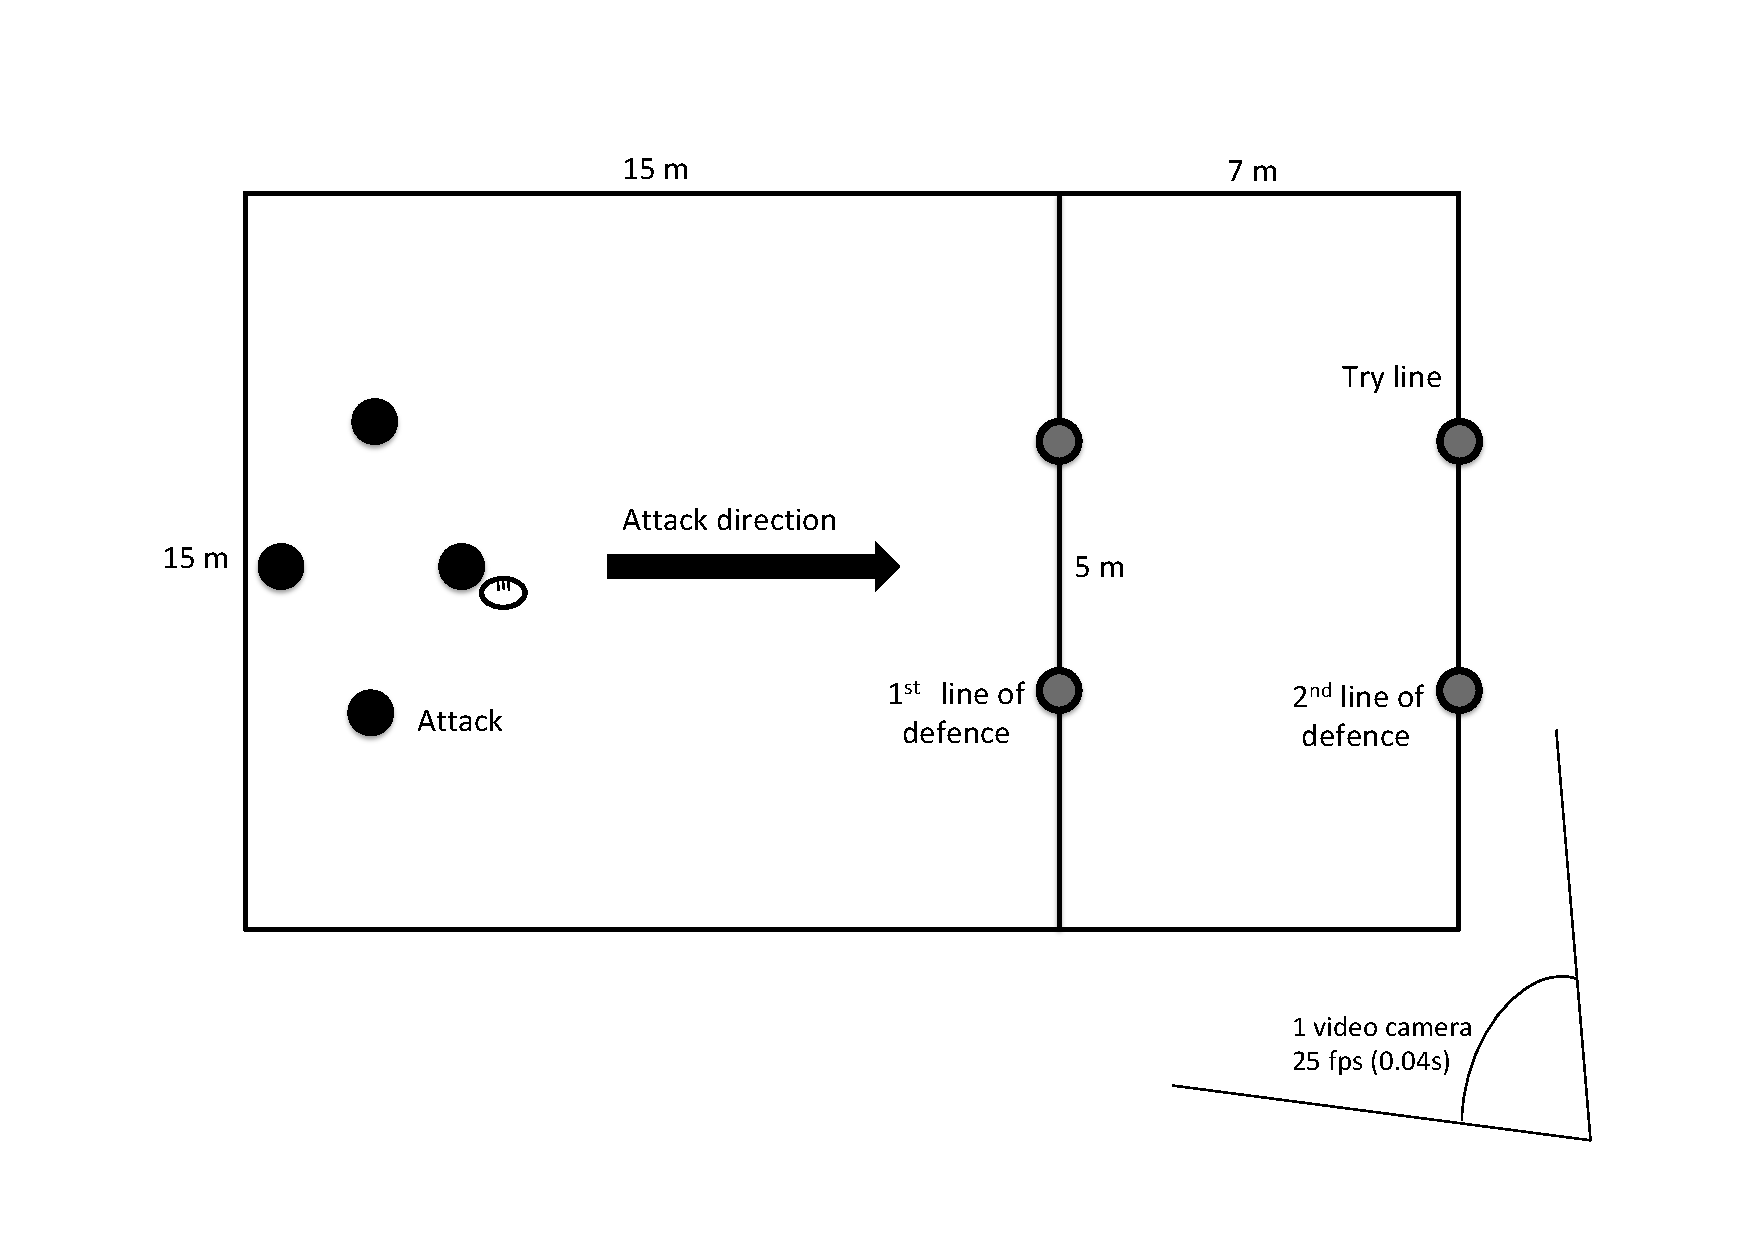
\includegraphics[width = \linewidth]{/Users/jacob1/Documents/2017/Research/DPhil/Dissertation/finalDocuments/jointActionSocialBonding/images/invasionDrill.pdf}
  \caption{The Invasion Drill, adapted from Passos (2011)}
  \label{fig:invasionDrill}
\end{figure}

\subsubsection{Experimental Paradigm: Invasion Drill}
This study required athletes to participate in a common rugby training drill, which was preceeded by one of two experimental primes—--a ``high difficulty'' condition, or a ``low difficulty'' condition.   Replicating \textcite{Passos2011}, a common training drill known as ``invasion drill'' \citep{Biscombe1998} was selected as it was representative of a typical subphase of joint action in rugby union.
In this drill, a group of four rugby players form an attacking group and two pairs of opponents form a first and second defensive line.  There were two performance aims of this drill: (a) attackers were asked carry the ball into the try area, and (b) defenders were asked to stop the attacker’s progression toward the try line.
One trial consisted of one attempt by the attacking sub-group to penetrate two defending sub-groups, and carry the ball over the try line. The drill was conducted on a regulation multipurpose 110m x 70m grass or artificial turf training field within a 22m x 15m rectangle area marked by plastic cones (see Figure ~\ref{fig:invasionDrill}). The ball used was size 5, as recommended by World Rugby for this age group of athletes.

%The training drill, known as ``invasion drill,'' requires eight athletes, one sub-grouof four attackers and two sub-groups of two defenders.  The primary aim of the drill is for the sub-group of 4 attacking players to successfully penetrate two consecutive lines of two defenders (also commonly known as a ``4 on 2 + 2'' drill). The aim of the two defending sub-groups is to stop the attacking team from achieving the primary goal, by interfering with their coordination by halting the ball-carrier, or the ball in flight between attacking players.


\subsubsection{Experimental Conditions: high and low difficulty}
Two different pre-experiment primes were developed for the same training drill in order to manipulate athletes’ expectations around the technical difficulty of the impending joint-action task.  Athletes in the ``high difficulty'' condition learned that the overall average difficulty rating for the training drill, provided by World Rugby coaches and athletes, was 77.5/100, or approximately 8 out of 10.  Athletes were told that the drill would require an extension of their abilities as individuals and as a training group (see appendix for full script).  Athletes in the ``low difficulty'' condition, by contrast, learned that they would be participating in an ostensibly different drill with an overall average difficulty rating (provided by World Rugby coaches and athletes) of 22.5/100, or approximately 2 out of 10.  In reality, the training drill was exactly the same for each experimental session, and the relative difficulty of this drill was estimated in a pilot study to be approximately 5/10, see APPENDIX).  By either over- or under-rating the difficulty of the impending training drill, athletes' expectations around certainty of performance would be altered, such that athletes in the high difficulty condition would experience on average higher (positive) violation of expectations around team performance, whereas athletes in the low difficulty condition would on average perceive team performance less positively relative to prior of expectations. Surveys were designed and administered using Qualtrics software (Qualtrics version 9, Provo, UT). Survey data were processed and analysed using the R environment (R Development Core Team, 2006).


\subsubsection{Measures}

\myparagraph{Surveys}
Surveys were administered at three time points: 1) one day before the experiment (Baseline), 2) immediately before the experiment after receiving the experimental prime (Pre-Experiment), and 3) once immediately following the completion of the experiment (Post-Experiment)(see ~\ref{tab:surveyItemsByTime}).  Consistent with the previous study (Chapter 8), athletes responded to questions about 1) perceptions of components and overall individual and team performance in joint action, 2) feelings associated with ``team click'' in joint action, and feelings of social bonding and group membership.  In addition, athletes responded to survey items designed to measure possible moderators of the relationship between joint action and social bonding, namely: perceptions of arousal, fatigue, injury status, and personality type.

At Baseline, athletes were asked about their impressions of recent individual performance and the performance of their province team as a whole.  Survey items included questions relating to specific components of on-field performance (e.g., team components: Attack, defence, onfield communication, and support play; individual components: Passing technique, one-on-one tackling, effectiveness in contact areas) as well as items relating to overall impressions of performance, for example: ``How well do you feel your team has been performing in training and competition over the past month?'' (100 point scale, 0 = ``Extremely bad'', 100 = ``Extremely good'').  Athletes also responded to questions about feelings of team click and social bonding with their team as a whole. In addition, the Baseline survey also included items concerning basic personal information, current injury status, subjective and objective measures of tehcnical competence, and personality type.
For a full explanation of survey items measured at Baseline, see Chapter 6 (Introduction to Part B) and Appendix ~\ref{} Section ~\ref{}.

At time 2, immediately prior to the experiment (Pre-Experiment), athletes were asked questions about feelings and expectations concerning their individual performance and the performance of their specific training group in the impending training drill.
For example,  athletes were asked ``How do you feel \textit{right now} about your individual performance (100 point scale, 0 = ``Extremely bad'', 100 = ``Extremely good'')''.  Athletes were also asked a series of questions about feelings of team click and social bonding to their specific training group. For team click, for example, athletes were asked questions like: ``How do you feel the tacit understanding is between the training group today?'' (100 point scale, 0 = ``Extremely bad'', 100 = ``Extremely good'').  For social bonding, athletes were asked questions like: ``How emotionally supportive does your training group feel right now?'' (100 point scale, 0 = ``Extremely weak'', 100 = ``Extremely strong'').
For a full explanation of survey items measured at Pre-Experiment, see Appendix ~\ref{} Section ~\ref{}.

At time 3, immediately after the completion of the experiment (Post-Experiment), athletes completed questions concerning their impression of their own performance and the performance of their training group in the training drill, relative to their prior expectations.  Athletes were also asked about their feelings of team click and social bonding to the training group as well as the provincial team as a whole (team-focussed questons mirrored the survey items that were asked one day earlier at Baseline).  For a full explanation of Post-Experiment survey items, see Appendix ~\ref{} Section ~\ref{}.

Surveys were generated in English by the researcher using Qualtrics software (Qualtrics version 9, Provo, UT). Surveys were translated into modern Chinese and back translated by two independent native Chinese speaking translators from Beijing Sports University to verify accuracy.  Athletes completed the modern Chinese version of each survey using WeChat on their personal mobile devices connected remotely to the internet.





\subsubsection{Video analysis of training group performance in training drill}
In order to produce quantitative measures of interpersonal coordination between co-actors, athletes’ motion was captured by a single digital video camera (Sony FDR-AX700 4K HDR Camcorder) mounted on a 1.2m high tripod. Digital video images of action were acquired by a computer, using a USB2.0 cable, and files were saved on an encrypted external hard disk in .AVI format. For image treatment, TACTO 8.0 software was used for digitizing at 25 frames per second.

Video footage from all 8 experiment sessions was analysed by an hypothesis blind research assistant.  Each experimental trial of the Invasion Drill (16 in total) was coded according to the quality of performance relative to the primary (attacking) goal of the drill, i.e., scoring a try by carrying the ball over the try line.  A maximum value of 6 was awarded to a ``clear try'' (trials in which a clear unobstructed try was scored by the attacking sub-unit); 5 to a ``rough try'' (the ball-carrier crossed the try-line following some minimal level of physical contact or obstruction from the defence that did not halt the momentum of the attacking phase); 4 to an ``Obstructed try'' (a trial in which a try is scored, but the momentum of the attacking sub-unit was clearly interrupted); 3 to a ``no try - defence''  (a trial in which a ball carrier is completely obstructed by a defender, and the trial is unsuccessful largely due to the effecticeness of the defence); 2 to a ``no try - defence forced error'' (unsuccessful trial due to a combination of the defence and error in attack); 1 to a ``no try - unforced error'' (a failed trial due to an unforced error in attack).
For each experiment session, an average performance outcome (``Trial Outcome Average'') and the standard deviation of this outcome (``Trial Outcome SD'') was calculated in order to capture the central tendency and variability of performance for each training group.

\subsection{Procedure}
Permission to run the study was sought from the head coach of each of the four teams (Beijing men's, Beijing women's, Shandong men's, Shandong women's).  These coaches nominated athletes who were fit and able to complete the session without compromising their existing training schedules.  Athletes were randomly assigned to one of two conditions, and then athletes in each experimental group were subsequently adjusted subsequently so that each condition was matched as much as possible according to average training age. Once athletes were assigned to an experimental group, they were then added to a WeChat group populated by other training group members and the researcher.

\subsubsection{Cover Story}
Athletes were notified (first via WeChat and then in a team meeting) that they were participating in a trial of a number of different rugby training drills selected from a recent report by World Rugby concerning training methods for rugby sevens.  Athletes were told that the training drills had been previously rated by a selection of international level coaches and players from all over the world (including Asia and China).  Athletes were informed that the purpose of the exercise was for me to assess the ratings provided by World Rugby by replicating these drills with more rugby athletes in China.  Athletes were told that survey measures and video footage would be collected, which would be later analysed to assess individual performance of athletes in each training drill.  It was also explained to athletes that there would be a second round of drills also requiring groups of eight athletes, but the makeup of these groups may reshuffle depending on athletes preferences.  This detail allowed for the includion of a post-experiment bonding measure, in which athletes were asked to what extent they wished to continue to train with the same 8-athlete team in a subsequent round of drills.

Approximately 24 hours before the experiment session, athletes were instructed to complete the baseline survey by opening a link provided in the WeChat group.  This survey included written consent for the study. Approximately 1 hour before the experiment was due to take place, athletes were administered with an experimental prime via WeChat.  In the ``high difficulty'' condition, athletes were primed to believe that they were about to participate in a very difficult training drill (on the upper end of their individual and group technical abilities), whereas athletes in the ``low difficulty'' condition were primed to believe that they were about to participate in a relatively easy training drill well within their technical abilities (see APPENDIX for full script). All athletes were lead to believe that athletes in the other experiemntal groups were performing different drills to their assigned drill. In reality, the training drill for each condition was identical, the only thing that varied was the pre-experiment prime.

Once athletes were assembled at the designated training field, I verbally re-administered the same prime that had been sent to athletes via WeChat an hour earlier.  In addition, athletes were told in more detail about the requirements of the Invasion Drill (see APPENDIX for full details).  Specifically, athletes were told that their performance in the experiment would be assessed based on subsequent video analysis.  I told athletes that they would be assessed based on their performance in attack, defense, and their ability to coordinate attack and defense with others.  Athletes were provided with no other explicit information regarding performance goals, besides completing the experimental drill to the best of their ability within the rules of rugby.

Athletes were then administered with the time 2 survey (Pre-experiment), which took approximately 3-5 minutes to complete.  After every athlete had finished the survey, athletes participated in a standard warm up routine lasting approximately 10 minutes, including slow jogging and dynamic stretching.  Athletes were instructed not to use the rugby ball during this period, which served to reduce the amount of incidental coordination and interaction between participants prior to the start of the experiment trials.  Once athletes had completed the warm up, the researcher assembled the group within the training drill area.  One athlete was randomly assigned to stand at each of 8 available plastic markers (6 in the case of the modified drills).  In this position, athletes were told once more about the structure and procedure for the training drill, in particular the way in which athletes were expected to rotate clockwise after every trial of the drill so that athletes did not habituate to certain positions or sub-units in the drill.

To begin the drill, the ball-carrier at the front and centre of the attack sub-group was instructed to tap the ball with his / her foot, before initiating the attacking sub-phase by advancing forward towards the defence sub-units.  In the case that the ball was immediately fumbled during the initiation of the trial, the training group was instructed to restart that trial and the trial in which the mistake was made was not counted.  Following a block of 4 practice trials, athletes were told by the researcher that the formal test was beginning.  The group of athletes then completed 16 trials of the drill, which allowed each athlete to complete four trials of attack and four trials of defence, in different positions.  Following completion of all 16 test trials, athletes were assembled by the researcher and thanked for their participation, before being sent to the sideline of the training field to complete the final post-experiment survey using their mobile devices.  Following the completion of this final survey, athletes were told that they would be informed within two days about the next experiment trial (in fact, no more experiments were taking place).

\myparagraph{Video Analysis Procedure}
The digital camera and tripod were positioned on a platform 2m above the level of the playing field, approximately 10-15m from the bottom try-line corner of the Invasion Drill perimeter (see figure ~\ref{fig:invasionDrill}).  The experimenter began video recording before the athletes arrived, and ceased recording after all athletes had left the training field following the experiment.  Digital video images of action were acquired by a computer, using a USB2.0 cable, and files were saved on an encrypted external hard disk in .AVI format.

%For image treatment, TACTO 8.0 software was used for digitizing at 25 frames per second.
%The procedure is how the study was carried out. It often works well to describe the procedure in terms of what the participants did rather than what the researchers did. For example, the participants gave their informed consent, read a set of instructions, completed a block of four practice trials, completed a block of 20 test trials, completed two questionnaires, and were debriefed and excused.
















%%%%%%%%%%%%%%%%%%%%%%%%%%%%%%%%%%%%%%%%%%%%%%%%%%%%%%RESULTS%%%%%%%%%%%%%%%%%%%%%%%%%%%%%%%%%%%%%%%%%%%%%%%%%%%%%%%%%%%%%%%%SECTION%%%%%%%%%%%%%%%%%%%%%%%%%%%%%%%%%%%%%%%%%%%%%%%%


\section{Results}
A total of 58 athletes participated in 8 experimental sessions. In one session (Shandong men's high difficulty condition) a research assistant stood in as a dummy participant for an athlete could not participate due to injury.  In the two sessions with Beijing women's team, due to failure of athletes to take part due to injury (3) or illness (2), the training drill was modified to a ``3 on 2 + 1'' drill, requiring only six athletes to complete instead of eight. In one of these experimental sessions, a female dummy participant was also required to fill in to make up a total of 6 athletes for the modified drill.  In both cases, dummy participants were competent ex-athletes who were naive to the predictions of the study.  Dummy participants did not participate in the survey responses before or after the session. Survey and video data of the remaining 58 participants was analysed.






\subsection{Descriptive Statistics}

\subsubsection{Participants}

\begin{knitrout}
\definecolor{shadecolor}{rgb}{0.969, 0.969, 0.969}\color{fgcolor}\begin{kframe}


{\ttfamily\noindent\color{warningcolor}{\#\# Warning in bind\_rows\_(x, .id): Unequal factor levels: coercing to character}}

{\ttfamily\noindent\color{warningcolor}{\#\# Warning in bind\_rows\_(x, .id): binding character and factor vector, coercing into character vector}}

{\ttfamily\noindent\color{warningcolor}{\#\# Warning in bind\_rows\_(x, .id): binding character and factor vector, coercing into character vector}}\end{kframe}
\end{knitrout}

% latex table generated in R 3.3.0 by xtable 1.8-2 package
% Thu Oct 12 22:18:22 2017
\begin{table}[ht]
\centering
\begin{tabular}{llccc}
  \hline
 & Items & Baseline & Pre & Post \\ 
  \hline
1 & IndPerformance & * & * & * \\ 
  2 & GroupPerformance &  & * & * \\ 
  3 & TeamPerformance & * &  &  \\ 
  4 & GroupClick &  & * & * \\ 
  5 & TeamClick & * &  & * \\ 
  6 & GroupBonding &  & * & * \\ 
  7 & TeamBonding & * &  & * \\ 
  8 & Arousal &  & * & * \\ 
  9 & Exertion &  &  & * \\ 
   \hline
\end{tabular}
\label{tab:athleteDescriptivesTrainingOverall}
\end{table}








The attributes of the overall sample of athletes are displayed in Table ~\ref{tab:athleteDescriptivesTrainingOverall}. The average training age of athletes was 4.2181818 years (2.1142454), with athletes having spent on average over 5.6363636 years in the team.
36\% of the sample were full-time employees of their provincial team, with the rest either being employed on a full-time (but fixed term) contract
(13.79\%)), a ``student contract'' ((27.59\%))), a short term training contract
((13.79\%))), or on a short-term trial basis ((3.45\%))).
 18 of 58 (31\%) of athletes declared that there were in the starting team of their respective provincial teams.
Attributes of athletes in the high and low difficulty conditions were evenly matched (see Table ~\ref{tab:athleteDescriptivesTrainingOverall}), with only a marginally significant difference in average age between conditions (high difficulty condition = 20.4814815(3.1054588), low difficulty condition = 22.1428571(3.3853091).

\subsubsection{Survey Responses}

Athlete responses to survey items were collated according to main variables of interest, particularly perceptions of individual and team performance in joint action, social variables relating to team click, social bonding, and moderator variables related to technical competence, arousal, exertion, and personality. In general, the central tendency of all survey items was between .5 to 1.5 standard deviations above the mid-point of the scale, with almost all survey item distributions exhibiting low to moderate negative skew.  Average athlete perceptions of individual (Appendix Tables ~\ref{tab:indPerfTimeLowTraining} and ~\ref{tab:indPerfTimeHighTraining}), group (Appendix Tables ~\ref{tab:groupPerfTimeLowTraining} and ~\ref{tab:groupPerfTimeHighTraining}), and team (measured at Baseline only, see Appendix Table ~\ref{tab:teamPerfTimeBaselineTraining}) performance ranged from a low of 58.31(17.71) for perceptions of individual performance relative to prior expectations (measured post-Experiment) to a high of 78.62 (12.75) for athlete confidence in group ability to meet the technical challenges of the drill, measured pre-Experiment.  Athletes were on average more critical in regards to perceptions of individual performance than they were of group and team performance, and were generally more critical of individual and group performance in the post-Experiment survey than they were in the Baseline and pre-Experiment surveys (see Appendix Tables ~\ref{tab:indPerfTimeLowTraining}\nobreakdash~\ref{tab:teamPerfTimeBaselineTraining}).

Central tendencies of variables measuring athletes' perceptions of group click and social bonding were also well above the mid-point of their respective scales, ranging from a low of 68.34 (SD = 14.69) for feelings of unspoken understanding measured post-Experiment in the low difficulty condition, to a high of 90.21 (SD = 9.33) for feelings of shared goal with the training group measured pre-Experiemnt in the low difficulty condition (see Appendix Tables ~\ref{tab:groupClickTimeHighTraining}\nobreakdash--\ref{tab:teamBondingTimeHighTraining}). Measures relating to Team Click and Social bonding also appeared to decrease in the post-Experiment survey relative to the pre-Experiment and Baseline surveys.  Objective measures of training group performance derived from video footage appeared to be consistent across experiment conditions (see Appendix Table ~\ref{tab:objectiveOutcomeCondition}).  For a description of the remaining moderator variables, see Appendix section ~\ref{}.

%%GROUP PERFORMANCE:
\begin{knitrout}
\definecolor{shadecolor}{rgb}{0.969, 0.969, 0.969}\color{fgcolor}\begin{kframe}


{\ttfamily\noindent\itshape\color{messagecolor}{\#\# \\\#\# Attaching package: 'scales'}}

{\ttfamily\noindent\itshape\color{messagecolor}{\#\# The following object is masked from 'package:purrr':\\\#\# \\\#\#\ \ \ \  discard}}

{\ttfamily\noindent\itshape\color{messagecolor}{\#\# The following object is masked from 'package:readr':\\\#\# \\\#\#\ \ \ \  col\_factor}}

{\ttfamily\noindent\color{warningcolor}{\#\# Warning in ModuleReturnVarsExist(vars, data): The data frame does not have: GroupPerformVsExpected\ \ Dropped}}

{\ttfamily\noindent\color{warningcolor}{\#\# Warning in min(x, na.rm = TRUE): no non-missing arguments to min; returning Inf}}

{\ttfamily\noindent\color{warningcolor}{\#\# Warning in min(x, na.rm = TRUE): no non-missing arguments to min; returning Inf}}

{\ttfamily\noindent\color{warningcolor}{\#\# Warning in min(x, na.rm = TRUE): no non-missing arguments to min; returning Inf}}

{\ttfamily\noindent\color{warningcolor}{\#\# Warning in min(x, na.rm = TRUE): no non-missing arguments to min; returning Inf}}

{\ttfamily\noindent\color{warningcolor}{\#\# Warning in min(x, na.rm = TRUE): no non-missing arguments to min; returning Inf}}

{\ttfamily\noindent\color{warningcolor}{\#\# Warning in max(x, na.rm = TRUE): no non-missing arguments to max; returning -Inf}}

{\ttfamily\noindent\color{warningcolor}{\#\# Warning in max(x, na.rm = TRUE): no non-missing arguments to max; returning -Inf}}

{\ttfamily\noindent\color{warningcolor}{\#\# Warning in max(x, na.rm = TRUE): no non-missing arguments to max; returning -Inf}}

{\ttfamily\noindent\color{warningcolor}{\#\# Warning in max(x, na.rm = TRUE): no non-missing arguments to max; returning -Inf}}

{\ttfamily\noindent\color{warningcolor}{\#\# Warning in max(x, na.rm = TRUE): no non-missing arguments to max; returning -Inf}}

{\ttfamily\noindent\color{warningcolor}{\#\# Warning in min(x, na.rm = TRUE): no non-missing arguments to min; returning Inf}}

{\ttfamily\noindent\color{warningcolor}{\#\# Warning in max(x, na.rm = TRUE): no non-missing arguments to max; returning -Inf}}

{\ttfamily\noindent\color{warningcolor}{\#\# Warning in StdDiff(variable = var, group = strataVar): Variable has only NA's in at least one stratum. na.rm turned off.}}

{\ttfamily\noindent\color{warningcolor}{\#\# Warning in StdDiff(variable = var, group = strataVar): Variable has only NA's in at least one stratum. na.rm turned off.}}

{\ttfamily\noindent\color{warningcolor}{\#\# Warning in StdDiff(variable = var, group = strataVar): Variable has only NA's in at least one stratum. na.rm turned off.}}

{\ttfamily\noindent\color{warningcolor}{\#\# Warning in StdDiff(variable = var, group = strataVar): Variable has only NA's in at least one stratum. na.rm turned off.}}

{\ttfamily\noindent\color{warningcolor}{\#\# Warning in StdDiff(variable = var, group = strataVar): Variable has only NA's in at least one stratum. na.rm turned off.}}

{\ttfamily\noindent\color{warningcolor}{\#\# Warning in ModuleReturnVarsExist(vars, data): The data frame does not have: GroupPerformVsExpected\ \ Dropped}}

{\ttfamily\noindent\color{warningcolor}{\#\# Warning in min(x, na.rm = TRUE): no non-missing arguments to min; returning Inf}}

{\ttfamily\noindent\color{warningcolor}{\#\# Warning in min(x, na.rm = TRUE): no non-missing arguments to min; returning Inf}}

{\ttfamily\noindent\color{warningcolor}{\#\# Warning in min(x, na.rm = TRUE): no non-missing arguments to min; returning Inf}}

{\ttfamily\noindent\color{warningcolor}{\#\# Warning in min(x, na.rm = TRUE): no non-missing arguments to min; returning Inf}}

{\ttfamily\noindent\color{warningcolor}{\#\# Warning in min(x, na.rm = TRUE): no non-missing arguments to min; returning Inf}}

{\ttfamily\noindent\color{warningcolor}{\#\# Warning in max(x, na.rm = TRUE): no non-missing arguments to max; returning -Inf}}

{\ttfamily\noindent\color{warningcolor}{\#\# Warning in max(x, na.rm = TRUE): no non-missing arguments to max; returning -Inf}}

{\ttfamily\noindent\color{warningcolor}{\#\# Warning in max(x, na.rm = TRUE): no non-missing arguments to max; returning -Inf}}

{\ttfamily\noindent\color{warningcolor}{\#\# Warning in max(x, na.rm = TRUE): no non-missing arguments to max; returning -Inf}}

{\ttfamily\noindent\color{warningcolor}{\#\# Warning in max(x, na.rm = TRUE): no non-missing arguments to max; returning -Inf}}

{\ttfamily\noindent\color{warningcolor}{\#\# Warning in min(x, na.rm = TRUE): no non-missing arguments to min; returning Inf}}

{\ttfamily\noindent\color{warningcolor}{\#\# Warning in max(x, na.rm = TRUE): no non-missing arguments to max; returning -Inf}}

{\ttfamily\noindent\color{warningcolor}{\#\# Warning in StdDiff(variable = var, group = strataVar): Variable has only NA's in at least one stratum. na.rm turned off.}}

{\ttfamily\noindent\color{warningcolor}{\#\# Warning in StdDiff(variable = var, group = strataVar): Variable has only NA's in at least one stratum. na.rm turned off.}}

{\ttfamily\noindent\color{warningcolor}{\#\# Warning in StdDiff(variable = var, group = strataVar): Variable has only NA's in at least one stratum. na.rm turned off.}}

{\ttfamily\noindent\color{warningcolor}{\#\# Warning in StdDiff(variable = var, group = strataVar): Variable has only NA's in at least one stratum. na.rm turned off.}}

{\ttfamily\noindent\color{warningcolor}{\#\# Warning in StdDiff(variable = var, group = strataVar): Variable has only NA's in at least one stratum. na.rm turned off.}}\end{kframe}
\end{knitrout}
%%IND PERFORMANCE
\begin{knitrout}
\definecolor{shadecolor}{rgb}{0.969, 0.969, 0.969}\color{fgcolor}\begin{kframe}


{\ttfamily\noindent\color{warningcolor}{\#\# Warning in min(x, na.rm = TRUE): no non-missing arguments to min; returning Inf}}

{\ttfamily\noindent\color{warningcolor}{\#\# Warning in min(x, na.rm = TRUE): no non-missing arguments to min; returning Inf}}

{\ttfamily\noindent\color{warningcolor}{\#\# Warning in max(x, na.rm = TRUE): no non-missing arguments to max; returning -Inf}}

{\ttfamily\noindent\color{warningcolor}{\#\# Warning in max(x, na.rm = TRUE): no non-missing arguments to max; returning -Inf}}

{\ttfamily\noindent\color{warningcolor}{\#\# Warning in min(x, na.rm = TRUE): no non-missing arguments to min; returning Inf}}

{\ttfamily\noindent\color{warningcolor}{\#\# Warning in max(x, na.rm = TRUE): no non-missing arguments to max; returning -Inf}}

{\ttfamily\noindent\color{warningcolor}{\#\# Warning in min(x, na.rm = TRUE): no non-missing arguments to min; returning Inf}}

{\ttfamily\noindent\color{warningcolor}{\#\# Warning in max(x, na.rm = TRUE): no non-missing arguments to max; returning -Inf}}

{\ttfamily\noindent\color{warningcolor}{\#\# Warning in StdDiff(variable = var, group = strataVar): Variable has only NA's in at least one stratum. na.rm turned off.}}

{\ttfamily\noindent\color{warningcolor}{\#\# Warning in StdDiff(variable = var, group = strataVar): Variable has only NA's in at least one stratum. na.rm turned off.}}

{\ttfamily\noindent\color{warningcolor}{\#\# Warning in StdDiff(variable = var, group = strataVar): Variable has only NA's in at least one stratum. na.rm turned off.}}

{\ttfamily\noindent\color{warningcolor}{\#\# Warning in min(x, na.rm = TRUE): no non-missing arguments to min; returning Inf}}

{\ttfamily\noindent\color{warningcolor}{\#\# Warning in min(x, na.rm = TRUE): no non-missing arguments to min; returning Inf}}

{\ttfamily\noindent\color{warningcolor}{\#\# Warning in max(x, na.rm = TRUE): no non-missing arguments to max; returning -Inf}}

{\ttfamily\noindent\color{warningcolor}{\#\# Warning in max(x, na.rm = TRUE): no non-missing arguments to max; returning -Inf}}

{\ttfamily\noindent\color{warningcolor}{\#\# Warning in min(x, na.rm = TRUE): no non-missing arguments to min; returning Inf}}

{\ttfamily\noindent\color{warningcolor}{\#\# Warning in max(x, na.rm = TRUE): no non-missing arguments to max; returning -Inf}}

{\ttfamily\noindent\color{warningcolor}{\#\# Warning in min(x, na.rm = TRUE): no non-missing arguments to min; returning Inf}}

{\ttfamily\noindent\color{warningcolor}{\#\# Warning in max(x, na.rm = TRUE): no non-missing arguments to max; returning -Inf}}

{\ttfamily\noindent\color{warningcolor}{\#\# Warning in StdDiff(variable = var, group = strataVar): Variable has only NA's in at least one stratum. na.rm turned off.}}

{\ttfamily\noindent\color{warningcolor}{\#\# Warning in StdDiff(variable = var, group = strataVar): Variable has only NA's in at least one stratum. na.rm turned off.}}

{\ttfamily\noindent\color{warningcolor}{\#\# Warning in StdDiff(variable = var, group = strataVar): Variable has only NA's in at least one stratum. na.rm turned off.}}\end{kframe}
\end{knitrout}
%GROUP CLICK:
\begin{knitrout}
\definecolor{shadecolor}{rgb}{0.969, 0.969, 0.969}\color{fgcolor}\begin{kframe}


{\ttfamily\noindent\color{warningcolor}{\#\# Warning in min(x, na.rm = TRUE): no non-missing arguments to min; returning Inf}}

{\ttfamily\noindent\color{warningcolor}{\#\# Warning in min(x, na.rm = TRUE): no non-missing arguments to min; returning Inf}}

{\ttfamily\noindent\color{warningcolor}{\#\# Warning in min(x, na.rm = TRUE): no non-missing arguments to min; returning Inf}}

{\ttfamily\noindent\color{warningcolor}{\#\# Warning in min(x, na.rm = TRUE): no non-missing arguments to min; returning Inf}}

{\ttfamily\noindent\color{warningcolor}{\#\# Warning in min(x, na.rm = TRUE): no non-missing arguments to min; returning Inf}}

{\ttfamily\noindent\color{warningcolor}{\#\# Warning in min(x, na.rm = TRUE): no non-missing arguments to min; returning Inf}}

{\ttfamily\noindent\color{warningcolor}{\#\# Warning in max(x, na.rm = TRUE): no non-missing arguments to max; returning -Inf}}

{\ttfamily\noindent\color{warningcolor}{\#\# Warning in max(x, na.rm = TRUE): no non-missing arguments to max; returning -Inf}}

{\ttfamily\noindent\color{warningcolor}{\#\# Warning in max(x, na.rm = TRUE): no non-missing arguments to max; returning -Inf}}

{\ttfamily\noindent\color{warningcolor}{\#\# Warning in max(x, na.rm = TRUE): no non-missing arguments to max; returning -Inf}}

{\ttfamily\noindent\color{warningcolor}{\#\# Warning in max(x, na.rm = TRUE): no non-missing arguments to max; returning -Inf}}

{\ttfamily\noindent\color{warningcolor}{\#\# Warning in max(x, na.rm = TRUE): no non-missing arguments to max; returning -Inf}}

{\ttfamily\noindent\color{warningcolor}{\#\# Warning in min(x, na.rm = TRUE): no non-missing arguments to min; returning Inf}}

{\ttfamily\noindent\color{warningcolor}{\#\# Warning in min(x, na.rm = TRUE): no non-missing arguments to min; returning Inf}}

{\ttfamily\noindent\color{warningcolor}{\#\# Warning in max(x, na.rm = TRUE): no non-missing arguments to max; returning -Inf}}

{\ttfamily\noindent\color{warningcolor}{\#\# Warning in max(x, na.rm = TRUE): no non-missing arguments to max; returning -Inf}}

{\ttfamily\noindent\color{warningcolor}{\#\# Warning in StdDiff(variable = var, group = strataVar): Variable has only NA's in at least one stratum. na.rm turned off.}}

{\ttfamily\noindent\color{warningcolor}{\#\# Warning in StdDiff(variable = var, group = strataVar): Variable has only NA's in at least one stratum. na.rm turned off.}}

{\ttfamily\noindent\color{warningcolor}{\#\# Warning in StdDiff(variable = var, group = strataVar): Variable has only NA's in at least one stratum. na.rm turned off.}}

{\ttfamily\noindent\color{warningcolor}{\#\# Warning in StdDiff(variable = var, group = strataVar): Variable has only NA's in at least one stratum. na.rm turned off.}}

{\ttfamily\noindent\color{warningcolor}{\#\# Warning in StdDiff(variable = var, group = strataVar): Variable has only NA's in at least one stratum. na.rm turned off.}}

{\ttfamily\noindent\color{warningcolor}{\#\# Warning in StdDiff(variable = var, group = strataVar): Variable has only NA's in at least one stratum. na.rm turned off.}}

{\ttfamily\noindent\color{warningcolor}{\#\# Warning in min(x, na.rm = TRUE): no non-missing arguments to min; returning Inf}}

{\ttfamily\noindent\color{warningcolor}{\#\# Warning in min(x, na.rm = TRUE): no non-missing arguments to min; returning Inf}}

{\ttfamily\noindent\color{warningcolor}{\#\# Warning in min(x, na.rm = TRUE): no non-missing arguments to min; returning Inf}}

{\ttfamily\noindent\color{warningcolor}{\#\# Warning in min(x, na.rm = TRUE): no non-missing arguments to min; returning Inf}}

{\ttfamily\noindent\color{warningcolor}{\#\# Warning in min(x, na.rm = TRUE): no non-missing arguments to min; returning Inf}}

{\ttfamily\noindent\color{warningcolor}{\#\# Warning in min(x, na.rm = TRUE): no non-missing arguments to min; returning Inf}}

{\ttfamily\noindent\color{warningcolor}{\#\# Warning in max(x, na.rm = TRUE): no non-missing arguments to max; returning -Inf}}

{\ttfamily\noindent\color{warningcolor}{\#\# Warning in max(x, na.rm = TRUE): no non-missing arguments to max; returning -Inf}}

{\ttfamily\noindent\color{warningcolor}{\#\# Warning in max(x, na.rm = TRUE): no non-missing arguments to max; returning -Inf}}

{\ttfamily\noindent\color{warningcolor}{\#\# Warning in max(x, na.rm = TRUE): no non-missing arguments to max; returning -Inf}}

{\ttfamily\noindent\color{warningcolor}{\#\# Warning in max(x, na.rm = TRUE): no non-missing arguments to max; returning -Inf}}

{\ttfamily\noindent\color{warningcolor}{\#\# Warning in max(x, na.rm = TRUE): no non-missing arguments to max; returning -Inf}}

{\ttfamily\noindent\color{warningcolor}{\#\# Warning in min(x, na.rm = TRUE): no non-missing arguments to min; returning Inf}}

{\ttfamily\noindent\color{warningcolor}{\#\# Warning in min(x, na.rm = TRUE): no non-missing arguments to min; returning Inf}}

{\ttfamily\noindent\color{warningcolor}{\#\# Warning in max(x, na.rm = TRUE): no non-missing arguments to max; returning -Inf}}

{\ttfamily\noindent\color{warningcolor}{\#\# Warning in max(x, na.rm = TRUE): no non-missing arguments to max; returning -Inf}}

{\ttfamily\noindent\color{warningcolor}{\#\# Warning in StdDiff(variable = var, group = strataVar): Variable has only NA's in at least one stratum. na.rm turned off.}}

{\ttfamily\noindent\color{warningcolor}{\#\# Warning in StdDiff(variable = var, group = strataVar): Variable has only NA's in at least one stratum. na.rm turned off.}}

{\ttfamily\noindent\color{warningcolor}{\#\# Warning in StdDiff(variable = var, group = strataVar): Variable has only NA's in at least one stratum. na.rm turned off.}}

{\ttfamily\noindent\color{warningcolor}{\#\# Warning in StdDiff(variable = var, group = strataVar): Variable has only NA's in at least one stratum. na.rm turned off.}}

{\ttfamily\noindent\color{warningcolor}{\#\# Warning in StdDiff(variable = var, group = strataVar): Variable has only NA's in at least one stratum. na.rm turned off.}}

{\ttfamily\noindent\color{warningcolor}{\#\# Warning in StdDiff(variable = var, group = strataVar): Variable has only NA's in at least one stratum. na.rm turned off.}}\end{kframe}
\end{knitrout}
%GROUP BONDING:
\begin{knitrout}
\definecolor{shadecolor}{rgb}{0.969, 0.969, 0.969}\color{fgcolor}\begin{kframe}


{\ttfamily\noindent\color{warningcolor}{\#\# Warning in min(x, na.rm = TRUE): no non-missing arguments to min; returning Inf}}

{\ttfamily\noindent\color{warningcolor}{\#\# Warning in min(x, na.rm = TRUE): no non-missing arguments to min; returning Inf}}

{\ttfamily\noindent\color{warningcolor}{\#\# Warning in min(x, na.rm = TRUE): no non-missing arguments to min; returning Inf}}

{\ttfamily\noindent\color{warningcolor}{\#\# Warning in min(x, na.rm = TRUE): no non-missing arguments to min; returning Inf}}

{\ttfamily\noindent\color{warningcolor}{\#\# Warning in max(x, na.rm = TRUE): no non-missing arguments to max; returning -Inf}}

{\ttfamily\noindent\color{warningcolor}{\#\# Warning in max(x, na.rm = TRUE): no non-missing arguments to max; returning -Inf}}

{\ttfamily\noindent\color{warningcolor}{\#\# Warning in max(x, na.rm = TRUE): no non-missing arguments to max; returning -Inf}}

{\ttfamily\noindent\color{warningcolor}{\#\# Warning in max(x, na.rm = TRUE): no non-missing arguments to max; returning -Inf}}

{\ttfamily\noindent\color{warningcolor}{\#\# Warning in min(x, na.rm = TRUE): no non-missing arguments to min; returning Inf}}

{\ttfamily\noindent\color{warningcolor}{\#\# Warning in max(x, na.rm = TRUE): no non-missing arguments to max; returning -Inf}}

{\ttfamily\noindent\color{warningcolor}{\#\# Warning in StdDiff(variable = var, group = strataVar): Variable has only NA's in at least one stratum. na.rm turned off.}}

{\ttfamily\noindent\color{warningcolor}{\#\# Warning in StdDiff(variable = var, group = strataVar): Variable has only NA's in at least one stratum. na.rm turned off.}}

{\ttfamily\noindent\color{warningcolor}{\#\# Warning in StdDiff(variable = var, group = strataVar): Variable has only NA's in at least one stratum. na.rm turned off.}}

{\ttfamily\noindent\color{warningcolor}{\#\# Warning in StdDiff(variable = var, group = strataVar): Variable has only NA's in at least one stratum. na.rm turned off.}}

{\ttfamily\noindent\color{warningcolor}{\#\# Warning in min(x, na.rm = TRUE): no non-missing arguments to min; returning Inf}}

{\ttfamily\noindent\color{warningcolor}{\#\# Warning in min(x, na.rm = TRUE): no non-missing arguments to min; returning Inf}}

{\ttfamily\noindent\color{warningcolor}{\#\# Warning in min(x, na.rm = TRUE): no non-missing arguments to min; returning Inf}}

{\ttfamily\noindent\color{warningcolor}{\#\# Warning in min(x, na.rm = TRUE): no non-missing arguments to min; returning Inf}}

{\ttfamily\noindent\color{warningcolor}{\#\# Warning in max(x, na.rm = TRUE): no non-missing arguments to max; returning -Inf}}

{\ttfamily\noindent\color{warningcolor}{\#\# Warning in max(x, na.rm = TRUE): no non-missing arguments to max; returning -Inf}}

{\ttfamily\noindent\color{warningcolor}{\#\# Warning in max(x, na.rm = TRUE): no non-missing arguments to max; returning -Inf}}

{\ttfamily\noindent\color{warningcolor}{\#\# Warning in max(x, na.rm = TRUE): no non-missing arguments to max; returning -Inf}}

{\ttfamily\noindent\color{warningcolor}{\#\# Warning in min(x, na.rm = TRUE): no non-missing arguments to min; returning Inf}}

{\ttfamily\noindent\color{warningcolor}{\#\# Warning in max(x, na.rm = TRUE): no non-missing arguments to max; returning -Inf}}

{\ttfamily\noindent\color{warningcolor}{\#\# Warning in StdDiff(variable = var, group = strataVar): Variable has only NA's in at least one stratum. na.rm turned off.}}

{\ttfamily\noindent\color{warningcolor}{\#\# Warning in StdDiff(variable = var, group = strataVar): Variable has only NA's in at least one stratum. na.rm turned off.}}

{\ttfamily\noindent\color{warningcolor}{\#\# Warning in StdDiff(variable = var, group = strataVar): Variable has only NA's in at least one stratum. na.rm turned off.}}

{\ttfamily\noindent\color{warningcolor}{\#\# Warning in StdDiff(variable = var, group = strataVar): Variable has only NA's in at least one stratum. na.rm turned off.}}\end{kframe}
\end{knitrout}
%TEAM BONDING
\begin{knitrout}
\definecolor{shadecolor}{rgb}{0.969, 0.969, 0.969}\color{fgcolor}\begin{kframe}


{\ttfamily\noindent\color{warningcolor}{\#\# Warning in min(x, na.rm = TRUE): no non-missing arguments to min; returning Inf}}

{\ttfamily\noindent\color{warningcolor}{\#\# Warning in min(x, na.rm = TRUE): no non-missing arguments to min; returning Inf}}

{\ttfamily\noindent\color{warningcolor}{\#\# Warning in min(x, na.rm = TRUE): no non-missing arguments to min; returning Inf}}

{\ttfamily\noindent\color{warningcolor}{\#\# Warning in min(x, na.rm = TRUE): no non-missing arguments to min; returning Inf}}

{\ttfamily\noindent\color{warningcolor}{\#\# Warning in min(x, na.rm = TRUE): no non-missing arguments to min; returning Inf}}

{\ttfamily\noindent\color{warningcolor}{\#\# Warning in min(x, na.rm = TRUE): no non-missing arguments to min; returning Inf}}

{\ttfamily\noindent\color{warningcolor}{\#\# Warning in min(x, na.rm = TRUE): no non-missing arguments to min; returning Inf}}

{\ttfamily\noindent\color{warningcolor}{\#\# Warning in min(x, na.rm = TRUE): no non-missing arguments to min; returning Inf}}

{\ttfamily\noindent\color{warningcolor}{\#\# Warning in min(x, na.rm = TRUE): no non-missing arguments to min; returning Inf}}

{\ttfamily\noindent\color{warningcolor}{\#\# Warning in min(x, na.rm = TRUE): no non-missing arguments to min; returning Inf}}

{\ttfamily\noindent\color{warningcolor}{\#\# Warning in max(x, na.rm = TRUE): no non-missing arguments to max; returning -Inf}}

{\ttfamily\noindent\color{warningcolor}{\#\# Warning in max(x, na.rm = TRUE): no non-missing arguments to max; returning -Inf}}

{\ttfamily\noindent\color{warningcolor}{\#\# Warning in max(x, na.rm = TRUE): no non-missing arguments to max; returning -Inf}}

{\ttfamily\noindent\color{warningcolor}{\#\# Warning in max(x, na.rm = TRUE): no non-missing arguments to max; returning -Inf}}

{\ttfamily\noindent\color{warningcolor}{\#\# Warning in max(x, na.rm = TRUE): no non-missing arguments to max; returning -Inf}}

{\ttfamily\noindent\color{warningcolor}{\#\# Warning in max(x, na.rm = TRUE): no non-missing arguments to max; returning -Inf}}

{\ttfamily\noindent\color{warningcolor}{\#\# Warning in max(x, na.rm = TRUE): no non-missing arguments to max; returning -Inf}}

{\ttfamily\noindent\color{warningcolor}{\#\# Warning in max(x, na.rm = TRUE): no non-missing arguments to max; returning -Inf}}

{\ttfamily\noindent\color{warningcolor}{\#\# Warning in max(x, na.rm = TRUE): no non-missing arguments to max; returning -Inf}}

{\ttfamily\noindent\color{warningcolor}{\#\# Warning in max(x, na.rm = TRUE): no non-missing arguments to max; returning -Inf}}

{\ttfamily\noindent\color{warningcolor}{\#\# Warning in StdDiff(variable = var, group = strataVar): Variable has only NA's in at least one stratum. na.rm turned off.}}

{\ttfamily\noindent\color{warningcolor}{\#\# Warning in StdDiff(variable = var, group = strataVar): Variable has only NA's in at least one stratum. na.rm turned off.}}

{\ttfamily\noindent\color{warningcolor}{\#\# Warning in StdDiff(variable = var, group = strataVar): Variable has only NA's in at least one stratum. na.rm turned off.}}

{\ttfamily\noindent\color{warningcolor}{\#\# Warning in StdDiff(variable = var, group = strataVar): Variable has only NA's in at least one stratum. na.rm turned off.}}

{\ttfamily\noindent\color{warningcolor}{\#\# Warning in StdDiff(variable = var, group = strataVar): Variable has only NA's in at least one stratum. na.rm turned off.}}

{\ttfamily\noindent\color{warningcolor}{\#\# Warning in StdDiff(variable = var, group = strataVar): Variable has only NA's in at least one stratum. na.rm turned off.}}

{\ttfamily\noindent\color{warningcolor}{\#\# Warning in StdDiff(variable = var, group = strataVar): Variable has only NA's in at least one stratum. na.rm turned off.}}

{\ttfamily\noindent\color{warningcolor}{\#\# Warning in StdDiff(variable = var, group = strataVar): Variable has only NA's in at least one stratum. na.rm turned off.}}

{\ttfamily\noindent\color{warningcolor}{\#\# Warning in StdDiff(variable = var, group = strataVar): Variable has only NA's in at least one stratum. na.rm turned off.}}

{\ttfamily\noindent\color{warningcolor}{\#\# Warning in StdDiff(variable = var, group = strataVar): Variable has only NA's in at least one stratum. na.rm turned off.}}

{\ttfamily\noindent\color{warningcolor}{\#\# Warning in min(x, na.rm = TRUE): no non-missing arguments to min; returning Inf}}

{\ttfamily\noindent\color{warningcolor}{\#\# Warning in min(x, na.rm = TRUE): no non-missing arguments to min; returning Inf}}

{\ttfamily\noindent\color{warningcolor}{\#\# Warning in min(x, na.rm = TRUE): no non-missing arguments to min; returning Inf}}

{\ttfamily\noindent\color{warningcolor}{\#\# Warning in min(x, na.rm = TRUE): no non-missing arguments to min; returning Inf}}

{\ttfamily\noindent\color{warningcolor}{\#\# Warning in min(x, na.rm = TRUE): no non-missing arguments to min; returning Inf}}

{\ttfamily\noindent\color{warningcolor}{\#\# Warning in min(x, na.rm = TRUE): no non-missing arguments to min; returning Inf}}

{\ttfamily\noindent\color{warningcolor}{\#\# Warning in min(x, na.rm = TRUE): no non-missing arguments to min; returning Inf}}

{\ttfamily\noindent\color{warningcolor}{\#\# Warning in min(x, na.rm = TRUE): no non-missing arguments to min; returning Inf}}

{\ttfamily\noindent\color{warningcolor}{\#\# Warning in min(x, na.rm = TRUE): no non-missing arguments to min; returning Inf}}

{\ttfamily\noindent\color{warningcolor}{\#\# Warning in min(x, na.rm = TRUE): no non-missing arguments to min; returning Inf}}

{\ttfamily\noindent\color{warningcolor}{\#\# Warning in max(x, na.rm = TRUE): no non-missing arguments to max; returning -Inf}}

{\ttfamily\noindent\color{warningcolor}{\#\# Warning in max(x, na.rm = TRUE): no non-missing arguments to max; returning -Inf}}

{\ttfamily\noindent\color{warningcolor}{\#\# Warning in max(x, na.rm = TRUE): no non-missing arguments to max; returning -Inf}}

{\ttfamily\noindent\color{warningcolor}{\#\# Warning in max(x, na.rm = TRUE): no non-missing arguments to max; returning -Inf}}

{\ttfamily\noindent\color{warningcolor}{\#\# Warning in max(x, na.rm = TRUE): no non-missing arguments to max; returning -Inf}}

{\ttfamily\noindent\color{warningcolor}{\#\# Warning in max(x, na.rm = TRUE): no non-missing arguments to max; returning -Inf}}

{\ttfamily\noindent\color{warningcolor}{\#\# Warning in max(x, na.rm = TRUE): no non-missing arguments to max; returning -Inf}}

{\ttfamily\noindent\color{warningcolor}{\#\# Warning in max(x, na.rm = TRUE): no non-missing arguments to max; returning -Inf}}

{\ttfamily\noindent\color{warningcolor}{\#\# Warning in max(x, na.rm = TRUE): no non-missing arguments to max; returning -Inf}}

{\ttfamily\noindent\color{warningcolor}{\#\# Warning in max(x, na.rm = TRUE): no non-missing arguments to max; returning -Inf}}

{\ttfamily\noindent\color{warningcolor}{\#\# Warning in StdDiff(variable = var, group = strataVar): Variable has only NA's in at least one stratum. na.rm turned off.}}

{\ttfamily\noindent\color{warningcolor}{\#\# Warning in StdDiff(variable = var, group = strataVar): Variable has only NA's in at least one stratum. na.rm turned off.}}

{\ttfamily\noindent\color{warningcolor}{\#\# Warning in StdDiff(variable = var, group = strataVar): Variable has only NA's in at least one stratum. na.rm turned off.}}

{\ttfamily\noindent\color{warningcolor}{\#\# Warning in StdDiff(variable = var, group = strataVar): Variable has only NA's in at least one stratum. na.rm turned off.}}

{\ttfamily\noindent\color{warningcolor}{\#\# Warning in StdDiff(variable = var, group = strataVar): Variable has only NA's in at least one stratum. na.rm turned off.}}

{\ttfamily\noindent\color{warningcolor}{\#\# Warning in StdDiff(variable = var, group = strataVar): Variable has only NA's in at least one stratum. na.rm turned off.}}

{\ttfamily\noindent\color{warningcolor}{\#\# Warning in StdDiff(variable = var, group = strataVar): Variable has only NA's in at least one stratum. na.rm turned off.}}

{\ttfamily\noindent\color{warningcolor}{\#\# Warning in StdDiff(variable = var, group = strataVar): Variable has only NA's in at least one stratum. na.rm turned off.}}

{\ttfamily\noindent\color{warningcolor}{\#\# Warning in StdDiff(variable = var, group = strataVar): Variable has only NA's in at least one stratum. na.rm turned off.}}

{\ttfamily\noindent\color{warningcolor}{\#\# Warning in StdDiff(variable = var, group = strataVar): Variable has only NA's in at least one stratum. na.rm turned off.}}\end{kframe}
\end{knitrout}
%%IND PERFORMANCE SUBJECTIVE:

%%OBJECTIVE OUTCOME:
\begin{knitrout}
\definecolor{shadecolor}{rgb}{0.969, 0.969, 0.969}\color{fgcolor}\begin{kframe}


{\ttfamily\noindent\bfseries\color{errorcolor}{\#\# Error: `fullOutcomeAvg`, `outcomeSD` contains unknown variables}}

{\ttfamily\noindent\color{warningcolor}{\#\# Warning in ModuleReturnVarsExist(vars, data): The data frame does not have: TrialOutcomeAvg\ \ Dropped}}

{\ttfamily\noindent\bfseries\color{errorcolor}{\#\# Error in ModuleStopIfNoVarsLeft(vars): No valid variables.}}\end{kframe}
\end{knitrout}
%TEAM DISCIPLINE:
\begin{knitrout}
\definecolor{shadecolor}{rgb}{0.969, 0.969, 0.969}\color{fgcolor}\begin{kframe}


{\ttfamily\noindent\color{warningcolor}{\#\# Warning in min(x, na.rm = TRUE): no non-missing arguments to min; returning Inf}}

{\ttfamily\noindent\color{warningcolor}{\#\# Warning in min(x, na.rm = TRUE): no non-missing arguments to min; returning Inf}}

{\ttfamily\noindent\color{warningcolor}{\#\# Warning in min(x, na.rm = TRUE): no non-missing arguments to min; returning Inf}}

{\ttfamily\noindent\color{warningcolor}{\#\# Warning in min(x, na.rm = TRUE): no non-missing arguments to min; returning Inf}}

{\ttfamily\noindent\color{warningcolor}{\#\# Warning in max(x, na.rm = TRUE): no non-missing arguments to max; returning -Inf}}

{\ttfamily\noindent\color{warningcolor}{\#\# Warning in max(x, na.rm = TRUE): no non-missing arguments to max; returning -Inf}}

{\ttfamily\noindent\color{warningcolor}{\#\# Warning in max(x, na.rm = TRUE): no non-missing arguments to max; returning -Inf}}

{\ttfamily\noindent\color{warningcolor}{\#\# Warning in max(x, na.rm = TRUE): no non-missing arguments to max; returning -Inf}}

{\ttfamily\noindent\color{warningcolor}{\#\# Warning in StdDiff(variable = var, group = strataVar): Variable has only NA's in at least one stratum. na.rm turned off.}}

{\ttfamily\noindent\color{warningcolor}{\#\# Warning in StdDiff(variable = var, group = strataVar): Variable has only NA's in at least one stratum. na.rm turned off.}}

{\ttfamily\noindent\color{warningcolor}{\#\# Warning in StdDiff(variable = var, group = strataVar): Variable has only NA's in at least one stratum. na.rm turned off.}}

{\ttfamily\noindent\color{warningcolor}{\#\# Warning in StdDiff(variable = var, group = strataVar): Variable has only NA's in at least one stratum. na.rm turned off.}}

{\ttfamily\noindent\color{warningcolor}{\#\# Warning in min(x, na.rm = TRUE): no non-missing arguments to min; returning Inf}}

{\ttfamily\noindent\color{warningcolor}{\#\# Warning in min(x, na.rm = TRUE): no non-missing arguments to min; returning Inf}}

{\ttfamily\noindent\color{warningcolor}{\#\# Warning in min(x, na.rm = TRUE): no non-missing arguments to min; returning Inf}}

{\ttfamily\noindent\color{warningcolor}{\#\# Warning in min(x, na.rm = TRUE): no non-missing arguments to min; returning Inf}}

{\ttfamily\noindent\color{warningcolor}{\#\# Warning in max(x, na.rm = TRUE): no non-missing arguments to max; returning -Inf}}

{\ttfamily\noindent\color{warningcolor}{\#\# Warning in max(x, na.rm = TRUE): no non-missing arguments to max; returning -Inf}}

{\ttfamily\noindent\color{warningcolor}{\#\# Warning in max(x, na.rm = TRUE): no non-missing arguments to max; returning -Inf}}

{\ttfamily\noindent\color{warningcolor}{\#\# Warning in max(x, na.rm = TRUE): no non-missing arguments to max; returning -Inf}}

{\ttfamily\noindent\color{warningcolor}{\#\# Warning in StdDiff(variable = var, group = strataVar): Variable has only NA's in at least one stratum. na.rm turned off.}}

{\ttfamily\noindent\color{warningcolor}{\#\# Warning in StdDiff(variable = var, group = strataVar): Variable has only NA's in at least one stratum. na.rm turned off.}}

{\ttfamily\noindent\color{warningcolor}{\#\# Warning in StdDiff(variable = var, group = strataVar): Variable has only NA's in at least one stratum. na.rm turned off.}}

{\ttfamily\noindent\color{warningcolor}{\#\# Warning in StdDiff(variable = var, group = strataVar): Variable has only NA's in at least one stratum. na.rm turned off.}}\end{kframe}
\end{knitrout}
%AROUSAL/EXERTION:
\begin{knitrout}
\definecolor{shadecolor}{rgb}{0.969, 0.969, 0.969}\color{fgcolor}\begin{kframe}


{\ttfamily\noindent\color{warningcolor}{\#\# Warning in min(x, na.rm = TRUE): no non-missing arguments to min; returning Inf}}

{\ttfamily\noindent\color{warningcolor}{\#\# Warning in min(x, na.rm = TRUE): no non-missing arguments to min; returning Inf}}

{\ttfamily\noindent\color{warningcolor}{\#\# Warning in min(x, na.rm = TRUE): no non-missing arguments to min; returning Inf}}

{\ttfamily\noindent\color{warningcolor}{\#\# Warning in min(x, na.rm = TRUE): no non-missing arguments to min; returning Inf}}

{\ttfamily\noindent\color{warningcolor}{\#\# Warning in min(x, na.rm = TRUE): no non-missing arguments to min; returning Inf}}

{\ttfamily\noindent\color{warningcolor}{\#\# Warning in min(x, na.rm = TRUE): no non-missing arguments to min; returning Inf}}

{\ttfamily\noindent\color{warningcolor}{\#\# Warning in max(x, na.rm = TRUE): no non-missing arguments to max; returning -Inf}}

{\ttfamily\noindent\color{warningcolor}{\#\# Warning in max(x, na.rm = TRUE): no non-missing arguments to max; returning -Inf}}

{\ttfamily\noindent\color{warningcolor}{\#\# Warning in max(x, na.rm = TRUE): no non-missing arguments to max; returning -Inf}}

{\ttfamily\noindent\color{warningcolor}{\#\# Warning in max(x, na.rm = TRUE): no non-missing arguments to max; returning -Inf}}

{\ttfamily\noindent\color{warningcolor}{\#\# Warning in max(x, na.rm = TRUE): no non-missing arguments to max; returning -Inf}}

{\ttfamily\noindent\color{warningcolor}{\#\# Warning in max(x, na.rm = TRUE): no non-missing arguments to max; returning -Inf}}

{\ttfamily\noindent\color{warningcolor}{\#\# Warning in min(x, na.rm = TRUE): no non-missing arguments to min; returning Inf}}

{\ttfamily\noindent\color{warningcolor}{\#\# Warning in min(x, na.rm = TRUE): no non-missing arguments to min; returning Inf}}

{\ttfamily\noindent\color{warningcolor}{\#\# Warning in max(x, na.rm = TRUE): no non-missing arguments to max; returning -Inf}}

{\ttfamily\noindent\color{warningcolor}{\#\# Warning in max(x, na.rm = TRUE): no non-missing arguments to max; returning -Inf}}

{\ttfamily\noindent\color{warningcolor}{\#\# Warning in StdDiff(variable = var, group = strataVar): Variable has only NA's in at least one stratum. na.rm turned off.}}

{\ttfamily\noindent\color{warningcolor}{\#\# Warning in StdDiff(variable = var, group = strataVar): Variable has only NA's in at least one stratum. na.rm turned off.}}

{\ttfamily\noindent\color{warningcolor}{\#\# Warning in StdDiff(variable = var, group = strataVar): Variable has only NA's in at least one stratum. na.rm turned off.}}

{\ttfamily\noindent\color{warningcolor}{\#\# Warning in StdDiff(variable = var, group = strataVar): Variable has only NA's in at least one stratum. na.rm turned off.}}

{\ttfamily\noindent\color{warningcolor}{\#\# Warning in StdDiff(variable = var, group = strataVar): Variable has only NA's in at least one stratum. na.rm turned off.}}

{\ttfamily\noindent\color{warningcolor}{\#\# Warning in StdDiff(variable = var, group = strataVar): Variable has only NA's in at least one stratum. na.rm turned off.}}

{\ttfamily\noindent\color{warningcolor}{\#\# Warning in min(x, na.rm = TRUE): no non-missing arguments to min; returning Inf}}

{\ttfamily\noindent\color{warningcolor}{\#\# Warning in min(x, na.rm = TRUE): no non-missing arguments to min; returning Inf}}

{\ttfamily\noindent\color{warningcolor}{\#\# Warning in min(x, na.rm = TRUE): no non-missing arguments to min; returning Inf}}

{\ttfamily\noindent\color{warningcolor}{\#\# Warning in min(x, na.rm = TRUE): no non-missing arguments to min; returning Inf}}

{\ttfamily\noindent\color{warningcolor}{\#\# Warning in min(x, na.rm = TRUE): no non-missing arguments to min; returning Inf}}

{\ttfamily\noindent\color{warningcolor}{\#\# Warning in min(x, na.rm = TRUE): no non-missing arguments to min; returning Inf}}

{\ttfamily\noindent\color{warningcolor}{\#\# Warning in max(x, na.rm = TRUE): no non-missing arguments to max; returning -Inf}}

{\ttfamily\noindent\color{warningcolor}{\#\# Warning in max(x, na.rm = TRUE): no non-missing arguments to max; returning -Inf}}

{\ttfamily\noindent\color{warningcolor}{\#\# Warning in max(x, na.rm = TRUE): no non-missing arguments to max; returning -Inf}}

{\ttfamily\noindent\color{warningcolor}{\#\# Warning in max(x, na.rm = TRUE): no non-missing arguments to max; returning -Inf}}

{\ttfamily\noindent\color{warningcolor}{\#\# Warning in max(x, na.rm = TRUE): no non-missing arguments to max; returning -Inf}}

{\ttfamily\noindent\color{warningcolor}{\#\# Warning in max(x, na.rm = TRUE): no non-missing arguments to max; returning -Inf}}

{\ttfamily\noindent\color{warningcolor}{\#\# Warning in min(x, na.rm = TRUE): no non-missing arguments to min; returning Inf}}

{\ttfamily\noindent\color{warningcolor}{\#\# Warning in min(x, na.rm = TRUE): no non-missing arguments to min; returning Inf}}

{\ttfamily\noindent\color{warningcolor}{\#\# Warning in max(x, na.rm = TRUE): no non-missing arguments to max; returning -Inf}}

{\ttfamily\noindent\color{warningcolor}{\#\# Warning in max(x, na.rm = TRUE): no non-missing arguments to max; returning -Inf}}

{\ttfamily\noindent\color{warningcolor}{\#\# Warning in StdDiff(variable = var, group = strataVar): Variable has only NA's in at least one stratum. na.rm turned off.}}

{\ttfamily\noindent\color{warningcolor}{\#\# Warning in StdDiff(variable = var, group = strataVar): Variable has only NA's in at least one stratum. na.rm turned off.}}

{\ttfamily\noindent\color{warningcolor}{\#\# Warning in StdDiff(variable = var, group = strataVar): Variable has only NA's in at least one stratum. na.rm turned off.}}

{\ttfamily\noindent\color{warningcolor}{\#\# Warning in StdDiff(variable = var, group = strataVar): Variable has only NA's in at least one stratum. na.rm turned off.}}

{\ttfamily\noindent\color{warningcolor}{\#\# Warning in StdDiff(variable = var, group = strataVar): Variable has only NA's in at least one stratum. na.rm turned off.}}

{\ttfamily\noindent\color{warningcolor}{\#\# Warning in StdDiff(variable = var, group = strataVar): Variable has only NA's in at least one stratum. na.rm turned off.}}\end{kframe}
\end{knitrout}
%PERSONALITY:










\subsection{Data Reduction}
Exploratory factor analysis was used to reduce multicolinearity between variables while retaining as much variance as possible in the observed data \citep{Yong2013}.
%(EFA, appendix ~\ref{appendix:EFA})
Data reduction was performed on the survey items related to the main outcome variables of interest, namely team click and social bonding directed at the training group. The procedure for data reduction followed the method outlined in the previous empirical chapter (Chapter 8).  Moderator variables---technical competence (objective and subjective), components of individual and training group performance, arousal, exertion, and athlete perception of team discipline---were also reduced to factors (see APPENDIX \ref{} HYPERLINK for full description of method).  In addition, items relating to team click and social bonding directed at the provincial team as a whole (and not just the specific training group) were reduced to factors, in order to assess pre- to post-experiment variation in generalised bonding to the team.

\subsubsection{Group Performance relative to prior expectations}
The main predictor variable of interest, perceptions of training group performance relative to prior expectations, was a single item measure, and did not require data reduction.  Considering that the outcome variables of interest (factors) were transformed to standardized z-scores (mean = 0, SD = 1),perceptions of team performance relative to prior expectation was also standardised (mean = 0, SD = 1) for the purposes of equivalence of predictor and outcome variables in subsequent linear mixed effects modelling.

\subsubsection{Feelings of team click within the training group}
\begin{knitrout}
\definecolor{shadecolor}{rgb}{0.969, 0.969, 0.969}\color{fgcolor}

{\centering 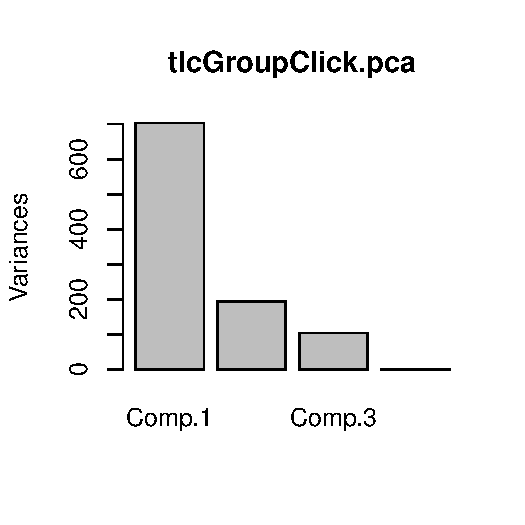
\includegraphics[width=\maxwidth]{/Users/jacob1/Documents/2017/Research/DPhil/Dissertation/finalDocuments/jointActionSocialBonding/images/dataReductionGroupClick-1} 

}



\end{knitrout}
%%Group click post has two extra variables that can be added (Reliability)
\begin{knitrout}
\definecolor{shadecolor}{rgb}{0.969, 0.969, 0.969}\color{fgcolor}

{\centering 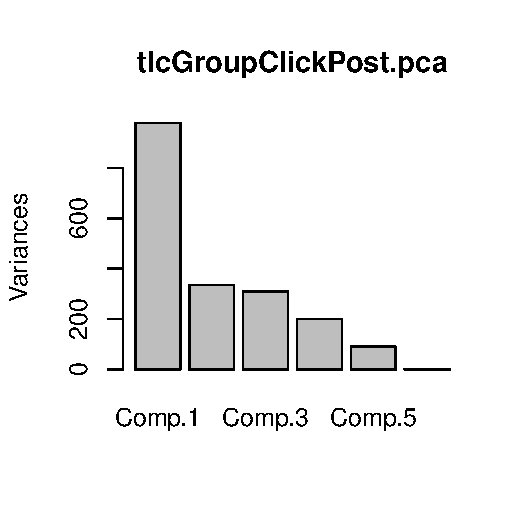
\includegraphics[width=\maxwidth]{/Users/jacob1/Documents/2017/Research/DPhil/Dissertation/finalDocuments/jointActionSocialBonding/images/dataReductionGroupClickPost-1} 

}



\end{knitrout}
\begin{knitrout}
\definecolor{shadecolor}{rgb}{0.969, 0.969, 0.969}\color{fgcolor}\begin{kframe}


{\ttfamily\noindent\itshape\color{messagecolor}{\#\# Loading required package: Hmisc}}

{\ttfamily\noindent\itshape\color{messagecolor}{\#\# Loading required package: lattice}}

{\ttfamily\noindent\itshape\color{messagecolor}{\#\# Loading required package: survival}}

{\ttfamily\noindent\itshape\color{messagecolor}{\#\# Loading required package: Formula}}

{\ttfamily\noindent\itshape\color{messagecolor}{\#\# \\\#\# Attaching package: 'Hmisc'}}

{\ttfamily\noindent\itshape\color{messagecolor}{\#\# The following objects are masked from 'package:xtable':\\\#\# \\\#\#\ \ \ \  label, label<-}}

{\ttfamily\noindent\itshape\color{messagecolor}{\#\# The following objects are masked from 'package:dplyr':\\\#\# \\\#\#\ \ \ \  src, summarize}}

{\ttfamily\noindent\itshape\color{messagecolor}{\#\# The following objects are masked from 'package:base':\\\#\# \\\#\#\ \ \ \  format.pval, units}}\end{kframe}
\end{knitrout}

Items relating to training group team click (unspoken understanding, general atmosphere, click pictorial, and ability extended by the group) were subjected to EFA.   Correlations between the remaining were very high (all r's > 0.2852293), which suggested that one factor was appropriate (see Table ee Table ~\ref{tab:groupClickCorrTable}). The KMO index and Bartlett's test both suggested high sampling adequacy, (KMO =  0.7245786, \chi^2(6, N = 116) = 127.8567081, p = \ensuremath{3.6325399\times 10^{-25}}).
One factor, labelled ``Group Click'' was imposed on the data, which explained 47.7\% of the overall variance (SS Loading = 2). Guttmans \lambda = 0.7338611 and Cronbachs \alpha = 0.7664883 indicated that the data reduction was appropriate and reliable.

In addition to the four variables common to both pre- and post-experiment surveys, athletes were also asked in the post-experiment survey about their own reliability and the reliability of other athletes to perform their role on the field specifically. These two variables, ``Reliability For Others'' and ``Reliability Of Others'' were included in an EFA involving only the post-experiment measures.  The variable ``reliability for others'' was removed from the matrix because it did not significantly correlate with other variables (all r's <= .16).

\subsubsection{Feelings of Social Bonding to the training group}
\begin{knitrout}
\definecolor{shadecolor}{rgb}{0.969, 0.969, 0.969}\color{fgcolor}

{\centering 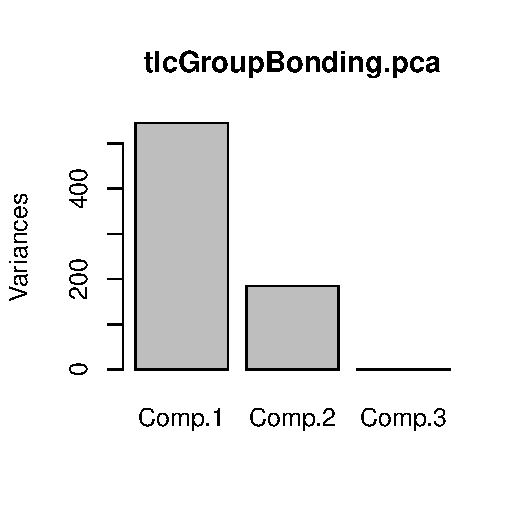
\includegraphics[width=\maxwidth]{/Users/jacob1/Documents/2017/Research/DPhil/Dissertation/finalDocuments/jointActionSocialBonding/images/dataReductionGroupBonding-1} 

}



\end{knitrout}

Items concerning bonding to the training group (emotional support, shared goal, fusion pictorial) were subjected to EFA.  Correlations between items were high (all r's > 0.3684898), which suggested that one factor would be appropriate (see Table ee Table ~\ref{tab:groupBondingCorrTable}). The KMO index and Bartlett's test both suggested high sampling adequacy, (KMO =  0.6501553, \chi^2(3, N = 116) = 54.2305691, p = \ensuremath{1.0019393\times 10^{-11}}).
One factor, labelled ``Group Social Bonding'' was imposed on the data, which explained 42\% of the overall variance (SS Loading = 1.26). Guttmans \lambda = 0.5877962 and Cronbachs \alpha = 0.6760861 indicated that the data reduction was appropriate and reliable.

\subsubsection{Additional data reduction}
In addition to athlete expectation violations concerning group and individual performance (predictor variable), group click (moderator and outcome variable), and group bonding (outcome variable), measures relating to athlete perceptions of components of group and individual performance, social bonding to the team as a whole, athlete arousal, technical competence (subjective and objective measures), and athlete perceptions of team discipline were subjected to data reduction (see Appendix Section ~\ref{} for full details).

\begin{knitrout}
\definecolor{shadecolor}{rgb}{0.969, 0.969, 0.969}\color{fgcolor}

{\centering 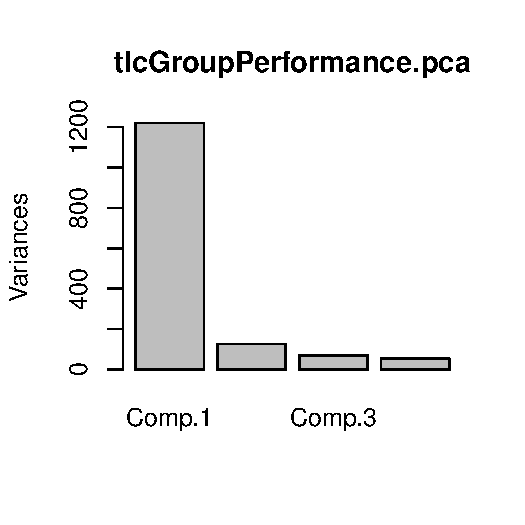
\includegraphics[width=\maxwidth]{/Users/jacob1/Documents/2017/Research/DPhil/Dissertation/finalDocuments/jointActionSocialBonding/images/dataReductionGroupPerformance-1} 

}



\end{knitrout}

\begin{knitrout}
\definecolor{shadecolor}{rgb}{0.969, 0.969, 0.969}\color{fgcolor}

{\centering 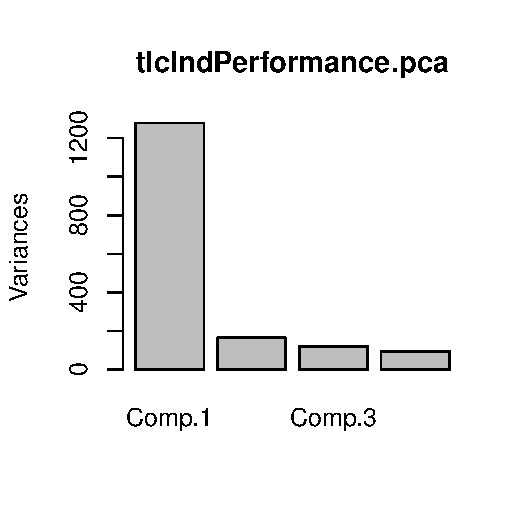
\includegraphics[width=\maxwidth]{/Users/jacob1/Documents/2017/Research/DPhil/Dissertation/finalDocuments/jointActionSocialBonding/images/dataReductionIndPerformance-1} 

}



\end{knitrout}











\begin{knitrout}
\definecolor{shadecolor}{rgb}{0.969, 0.969, 0.969}\color{fgcolor}\begin{kframe}


{\ttfamily\noindent\itshape\color{messagecolor}{\#\# \\\#\# Attaching package: 'psych'}}

{\ttfamily\noindent\itshape\color{messagecolor}{\#\# The following object is masked from 'package:Hmisc':\\\#\# \\\#\#\ \ \ \  describe}}

{\ttfamily\noindent\itshape\color{messagecolor}{\#\# The following objects are masked from 'package:scales':\\\#\# \\\#\#\ \ \ \  alpha, rescale}}

{\ttfamily\noindent\itshape\color{messagecolor}{\#\# The following object is masked from 'package:car':\\\#\# \\\#\#\ \ \ \  logit}}

{\ttfamily\noindent\itshape\color{messagecolor}{\#\# The following object is masked from 'package:mediation':\\\#\# \\\#\#\ \ \ \  mediate}}

{\ttfamily\noindent\itshape\color{messagecolor}{\#\# The following objects are masked from 'package:ggplot2':\\\#\# \\\#\#\ \ \ \  \%+\%, alpha}}\end{kframe}
\end{knitrout}











\subsection{Manipulation Checks}
The effectiveness of the experimental manipulation was assesed based on a comparison of athletes responses to three survey items immediately following the high or low difficulty prime and immediately before the training drill.
Athletes were asked about their confidence in their individual and training group's ability to handle the technical challenges of the training drill.
Due to the fact that athletes had been primed to expect either a difficult or simple training drill, it was expected that athletes in the high difficulty condition would be less confident about their own and their group's ability to meet the technical challenges of the training session.
In addition to self-reported confidence, it was also predicted that athlete self-reports of arousal, measured measured at the same time as the previous questions regarding confidence, would also vary according to condition.
It was predicted that that athletes in the high difficulty condition would be more aroused than athtletes in the low difficulty condition.  Meaningful variation in these variables could be used to check that the experimental manipulation was successful.









%%% group confidence in technical challenges:
\begin{knitrout}
\definecolor{shadecolor}{rgb}{0.969, 0.969, 0.969}\color{fgcolor}

{\centering 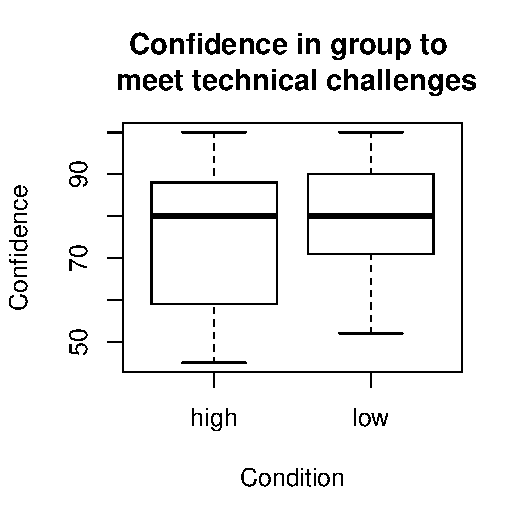
\includegraphics[width=\maxwidth]{/Users/jacob1/Documents/2017/Research/DPhil/Dissertation/finalDocuments/jointActionSocialBonding/images/groupConfChallengesBoxplot-1} 

}



\end{knitrout}
\begin{knitrout}
\definecolor{shadecolor}{rgb}{0.969, 0.969, 0.969}\color{fgcolor}

{\centering 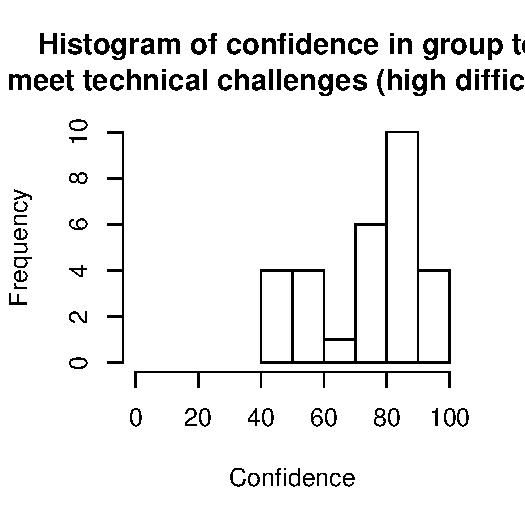
\includegraphics[width=\maxwidth]{/Users/jacob1/Documents/2017/Research/DPhil/Dissertation/finalDocuments/jointActionSocialBonding/images/histHighGroupConfidence-1} 

}



\end{knitrout}
\begin{knitrout}
\definecolor{shadecolor}{rgb}{0.969, 0.969, 0.969}\color{fgcolor}

{\centering 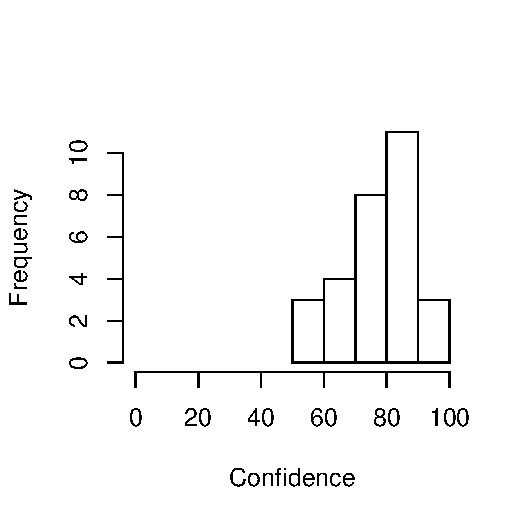
\includegraphics[width=\maxwidth]{/Users/jacob1/Documents/2017/Research/DPhil/Dissertation/finalDocuments/jointActionSocialBonding/images/histLowGroupConfidence-1} 

}



\end{knitrout}





\begin{knitrout}
\definecolor{shadecolor}{rgb}{0.969, 0.969, 0.969}\color{fgcolor}

{\centering 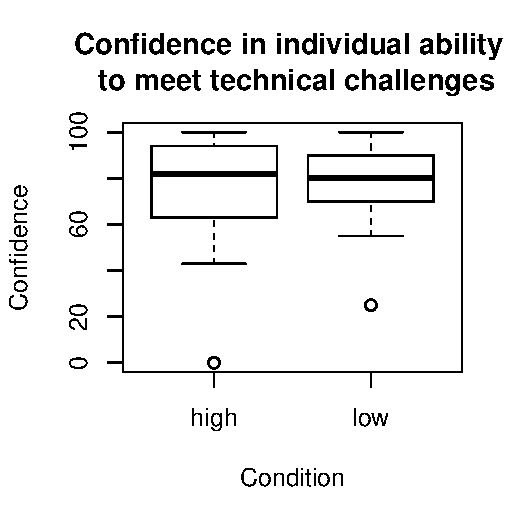
\includegraphics[width=\maxwidth]{/Users/jacob1/Documents/2017/Research/DPhil/Dissertation/finalDocuments/jointActionSocialBonding/images/indConfChallengesBoxplot-1} 

}



\end{knitrout}

\begin{knitrout}
\definecolor{shadecolor}{rgb}{0.969, 0.969, 0.969}\color{fgcolor}

{\centering 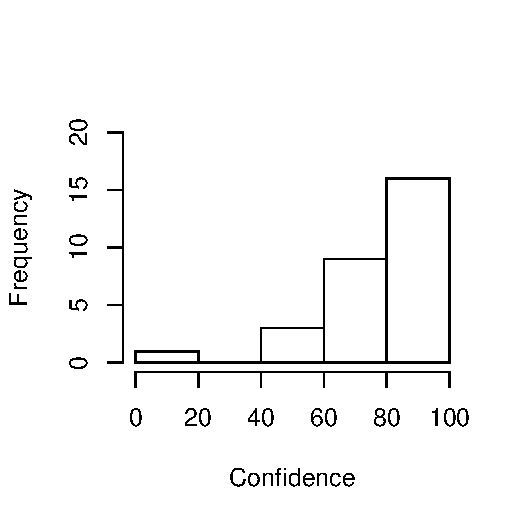
\includegraphics[width=\maxwidth]{/Users/jacob1/Documents/2017/Research/DPhil/Dissertation/finalDocuments/jointActionSocialBonding/images/histHighIndConfidence-1} 

}



\end{knitrout}

\begin{knitrout}
\definecolor{shadecolor}{rgb}{0.969, 0.969, 0.969}\color{fgcolor}

{\centering 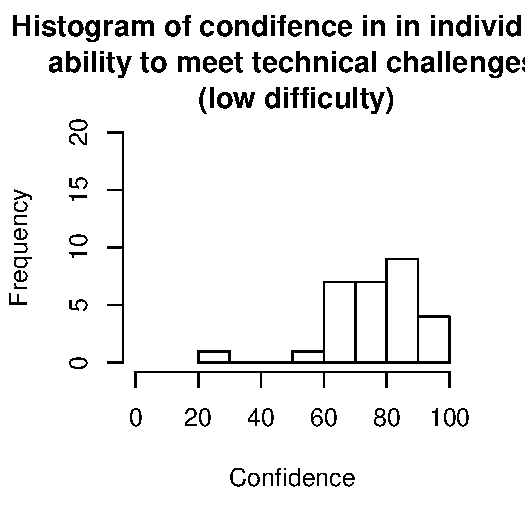
\includegraphics[width=\maxwidth]{/Users/jacob1/Documents/2017/Research/DPhil/Dissertation/finalDocuments/jointActionSocialBonding/images/histLowIndConfidence-1} 

}



\end{knitrout}


%(t_test(groupConfidenceCondition.ttest))
 %(t_test(indConfidenceCondition.ttest))
Results of manipulation checks indicate that there were no overall condition-wise differences in athlete confidence in group or individual ability to meet the technical challenges of the drill (see Table ~\ref{tab:manipulationCheckTable} and Figures ~\ref{fig:groupConfChallengesBoxplot} and ~\ref{fig:indConfChallengesBoxplot}).
Although the central tendency of these variables was not significantly different, the box plots (Figures ~\ref{fig:groupConfChallengesBoxplot}) and histograms of both group and individual confidence variables by condition show that the variance of responses in the high difficulty condition appears to be larger than the low difficulty condition (see Figures ~\ref{fig:histHighGroupConfidence}\nobreakdash~\ref{fig:histLowIndConfidence}).
A Bartlett's test of homogeneity of variance revealed that there was no meaningful difference in variance of confidence in group ability (c(`Bartlett's K-squared` = 2.39556133520555), c(df = 1), 0.12168006558935, groupConfidentTechnicalChallenges_2 by condition, Bartlett test of homogeneity of variances). The same test applied to athlete confidence in individual ability according to condition did, however, reveal a significant difference, c(`Bartlett's K-squared` = 4.042444164532), c(df = 1), 0.0443695168535268, indConfidenceChallenges_2 by condition, Bartlett test of homogeneity of variances.


\begin{knitrout}
\definecolor{shadecolor}{rgb}{0.969, 0.969, 0.969}\color{fgcolor}\begin{kframe}
\begin{alltt}
  \hlstd{arousalFactorPreBoxPlot} \hlkwb{<-} \hlkwd{boxplot}\hlstd{(arousalFactorPre} \hlopt{~} \hlstd{condition,}
                                        \hlkwc{varwidth} \hlstd{=} \hlnum{TRUE}\hlstd{,}
                                        \hlkwc{width} \hlstd{=} \hlkwd{c}\hlstd{(}\hlnum{.5}\hlstd{,}\hlnum{.5}\hlstd{),}
                                        \hlkwc{notch} \hlstd{= F,}
                                        \hlkwc{main} \hlstd{=} \hlnum{NA}\hlstd{,}
                                        \hlkwc{xlab} \hlstd{=} \hlstr{"Condition"}\hlstd{,}
                                        \hlkwc{ylab} \hlstd{=} \hlstr{"Arousal"}\hlstd{,}
                                        \hlkwc{data} \hlstd{= twc)}
\end{alltt}
\end{kframe}\begin{figure}

{\centering 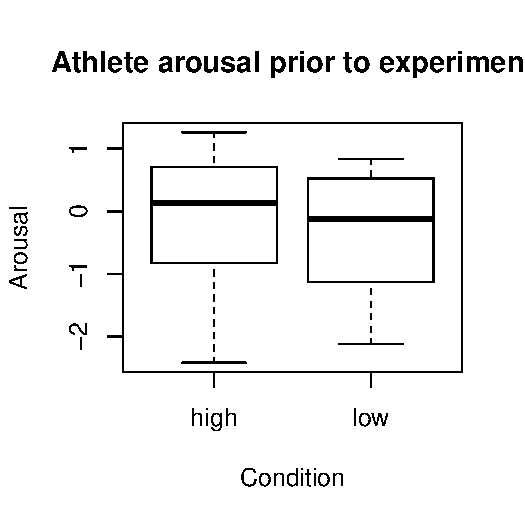
\includegraphics[width=\maxwidth]{/Users/jacob1/Documents/2017/Research/DPhil/Dissertation/finalDocuments/jointActionSocialBonding/images/arousalFactorPreBoxPlot-1} 

}

\end{figure}


\end{knitrout}

\begin{knitrout}
\definecolor{shadecolor}{rgb}{0.969, 0.969, 0.969}\color{fgcolor}\begin{kframe}
\begin{alltt}
  \hlstd{histArousalFactorPreHigh} \hlkwb{<-} \hlkwd{hist}\hlstd{(high}\hlopt{$}\hlstd{arousalFactorPre,}
                                        \hlkwc{main} \hlstd{=} \hlnum{NA}\hlstd{,}
                                        \hlkwc{xlab} \hlstd{=} \hlstr{"Arousal"}\hlstd{,}
                                        \hlkwc{xlim} \hlstd{=} \hlkwd{c}\hlstd{(}\hlopt{-}\hlnum{3}\hlstd{,} \hlnum{2}\hlstd{),}
                                        \hlkwc{ylim} \hlstd{=} \hlkwd{c}\hlstd{(}\hlnum{0}\hlstd{,}\hlnum{10}\hlstd{))}
\end{alltt}
\end{kframe}\begin{figure}

{\centering 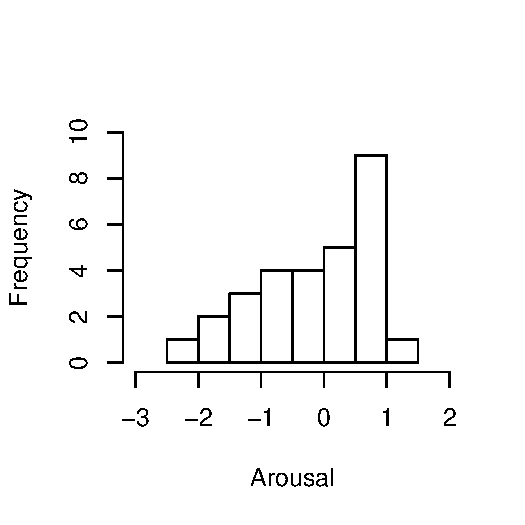
\includegraphics[width=\maxwidth]{/Users/jacob1/Documents/2017/Research/DPhil/Dissertation/finalDocuments/jointActionSocialBonding/images/histArousalFactorPreHigh-1} 

}

\end{figure}


\end{knitrout}

\begin{knitrout}
\definecolor{shadecolor}{rgb}{0.969, 0.969, 0.969}\color{fgcolor}\begin{kframe}
\begin{alltt}
  \hlkwd{hist}\hlstd{(low}\hlopt{$}\hlstd{arousalFactorPre,}
                              \hlkwc{main} \hlstd{=} \hlnum{NA}\hlstd{,}
                              \hlkwc{xlab} \hlstd{=} \hlstr{"Arousal"}\hlstd{,}
                              \hlkwc{xlim} \hlstd{=} \hlkwd{c}\hlstd{(}\hlopt{-}\hlnum{3}\hlstd{,} \hlnum{2}\hlstd{),}
                              \hlkwc{ylim} \hlstd{=} \hlkwd{c}\hlstd{(}\hlnum{0}\hlstd{,}\hlnum{10}\hlstd{))}
\end{alltt}
\end{kframe}\begin{figure}

{\centering 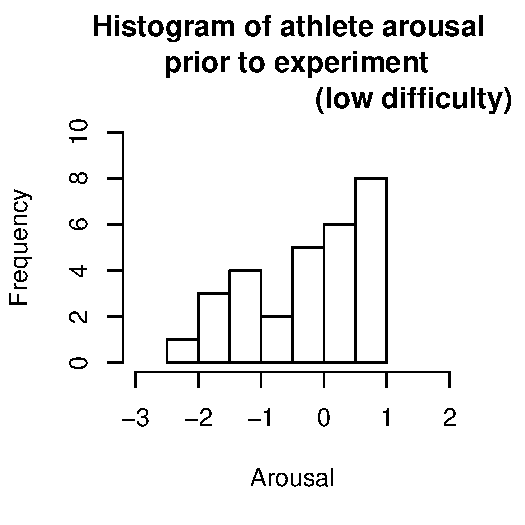
\includegraphics[width=\maxwidth]{/Users/jacob1/Documents/2017/Research/DPhil/Dissertation/finalDocuments/jointActionSocialBonding/images/histArousalFactorPreLow-1} 

}

\end{figure}


\end{knitrout}


%t_apa(arousalCondition.ttest)
An analysis of arousal by condition also failed to reveal meaningful variation by condition, (see Table ~\ref{tab:manipulationCheckTable} and Figure ~\ref{fig:arousalFactorPreBoxPlot}). Judging by the boxplot and histogram of each condition (see Figures ~\ref{fig:histArousalFactorPreHigh} and ~\ref{fig:histArousalFactorPreLow}), the variance of arousal in the high difficulty condition did appear to be higher than the low difficulty condition. A Bartlett's test for homogeneity of variance, however, revealed that the difference was not significant, c(`Bartlett's K-squared` = 0.46014520291942), c(df = 1), 0.497556120225506, arousalFactorPre by condition, Bartlett test of homogeneity of variances. These results suggested that the experimental prime was explicitly successful in significantly manipulating athlete self-reported confidence in individuala and group ability to meet the technical challenges associated with the training drill.  There was also no evidence that self-reported arousal differed significantly according to condition.
It was still possible, however, that the experimental primes influenced athletes implicitly, in ways that were not measured by surveys, which record explicit self-report.

\subsection{Results by condition}
Predictions of this study were first tested according to condition. It was predicted that the high difficulty prime would generate closer attention to the details of joint action between participants, and more positive violation of expectations around group performance.



%% jointACtionSuccess & indPerformance:
\begin{knitrout}
\definecolor{shadecolor}{rgb}{0.969, 0.969, 0.969}\color{fgcolor}\begin{kframe}
\begin{alltt}
  \hlstd{groupJointActionSuccessBoxPlot} \hlkwb{<-} \hlkwd{boxplot}\hlstd{(jointActionSuccessPost} \hlopt{~} \hlstd{condition,}
                                          \hlkwc{varwidth} \hlstd{=} \hlnum{TRUE}\hlstd{,}
                                          \hlkwc{width} \hlstd{=} \hlkwd{c}\hlstd{(}\hlnum{.5}\hlstd{,}\hlnum{.5}\hlstd{),}
                                          \hlkwc{notch} \hlstd{= F,}
                                          \hlkwc{main} \hlstd{=} \hlnum{NA}\hlstd{,}
                                          \hlkwc{xlab} \hlstd{=} \hlstr{"Condition"}\hlstd{,}
                                          \hlkwc{ylab} \hlstd{=} \hlstr{"Joint Action Success"}\hlstd{,}
                                          \hlkwc{data} \hlstd{= twc)}
\end{alltt}
\end{kframe}\begin{figure}

{\centering 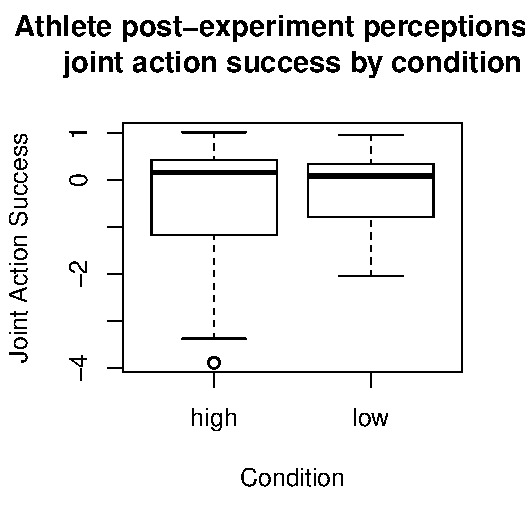
\includegraphics[width=\maxwidth]{/Users/jacob1/Documents/2017/Research/DPhil/Dissertation/finalDocuments/jointActionSocialBonding/images/groupJointActionSuccessPostBoxPlot-1} 

}

\end{figure}


\end{knitrout}
\begin{knitrout}
\definecolor{shadecolor}{rgb}{0.969, 0.969, 0.969}\color{fgcolor}\begin{kframe}
\begin{alltt}
  \hlstd{indComponentPerformancePostBoxPlot} \hlkwb{<-} \hlkwd{boxplot}\hlstd{(indPerformancePost} \hlopt{~} \hlstd{condition,}
                                          \hlkwc{varwidth} \hlstd{=} \hlnum{TRUE}\hlstd{,}
                                          \hlkwc{width} \hlstd{=} \hlkwd{c}\hlstd{(}\hlnum{.5}\hlstd{,}\hlnum{.5}\hlstd{),}
                                          \hlkwc{notch} \hlstd{= F,}
                                          \hlkwc{main} \hlstd{=} \hlnum{NA}\hlstd{,}
                                          \hlkwc{xlab} \hlstd{=} \hlstr{"Condition"}\hlstd{,}
                                          \hlkwc{ylab} \hlstd{=} \hlstr{"Individual Performance"}\hlstd{,}
                                          \hlkwc{data} \hlstd{= twc)}
\end{alltt}
\end{kframe}\begin{figure}

{\centering 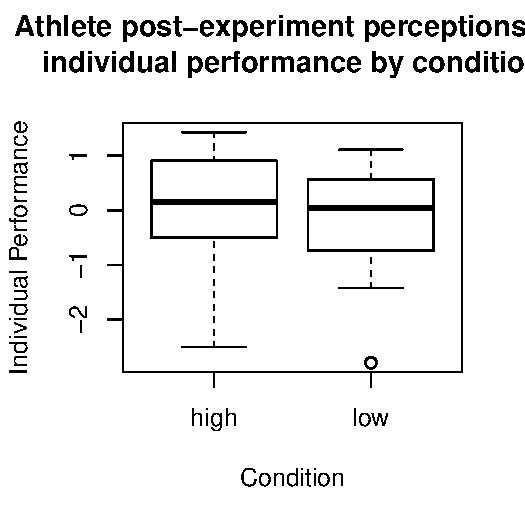
\includegraphics[width=\maxwidth]{/Users/jacob1/Documents/2017/Research/DPhil/Dissertation/finalDocuments/jointActionSocialBonding/images/indComponentPerformancePostBoxPlot-1} 

}

\end{figure}


\end{knitrout}
\begin{knitrout}
\definecolor{shadecolor}{rgb}{0.969, 0.969, 0.969}\color{fgcolor}\begin{kframe}
\begin{alltt}
  \hlstd{groupPerfExpPostBoxPlot} \hlkwb{<-} \hlkwd{boxplot}\hlstd{(groupPerformance_3Norm} \hlopt{~} \hlstd{condition,}
                                          \hlkwc{varwidth} \hlstd{=} \hlnum{TRUE}\hlstd{,}
                                          \hlkwc{width} \hlstd{=} \hlkwd{c}\hlstd{(}\hlnum{.5}\hlstd{,}\hlnum{.5}\hlstd{),}
                                          \hlkwc{notch} \hlstd{= F,}
                                          \hlkwc{xlab} \hlstd{=} \hlstr{"Condition"}\hlstd{,}
                                          \hlkwc{ylab} \hlstd{=} \hlstr{"Group Performance vs. Expectations"}\hlstd{,}
                                          \hlkwc{data} \hlstd{= twc)}
\end{alltt}
\end{kframe}\begin{figure}

{\centering 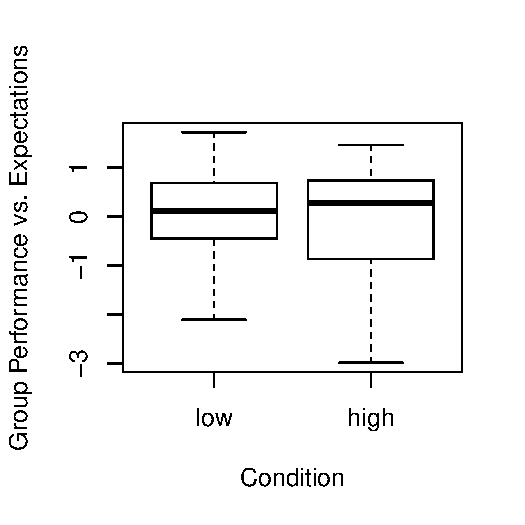
\includegraphics[width=\maxwidth]{/Users/jacob1/Documents/2017/Research/DPhil/Dissertation/finalDocuments/jointActionSocialBonding/images/groupPerfExpPostBoxPlot-1} 

}

\end{figure}


\end{knitrout}
\begin{knitrout}
\definecolor{shadecolor}{rgb}{0.969, 0.969, 0.969}\color{fgcolor}\begin{kframe}
\begin{alltt}
  \hlstd{indPerfExpPostBoxPlot} \hlkwb{<-} \hlkwd{boxplot}\hlstd{(indPerformance_3Norm} \hlopt{~} \hlstd{condition,}
                                          \hlkwc{varwidth} \hlstd{=} \hlnum{TRUE}\hlstd{,}
                                          \hlkwc{width} \hlstd{=} \hlkwd{c}\hlstd{(}\hlnum{.5}\hlstd{,}\hlnum{.5}\hlstd{),}
                                          \hlkwc{notch} \hlstd{= F,}
                                          \hlkwc{main} \hlstd{=} \hlnum{NA}\hlstd{,}
                                          \hlkwc{xlab} \hlstd{=} \hlstr{"Condition"}\hlstd{,}
                                          \hlkwc{ylab} \hlstd{=} \hlstr{"Individual Performance vs. Expectations"}\hlstd{,}
                                          \hlkwc{data} \hlstd{= twc)}
\end{alltt}
\end{kframe}\begin{figure}

{\centering 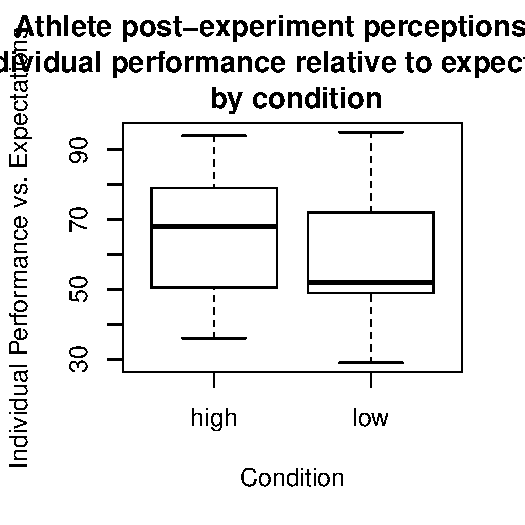
\includegraphics[width=\maxwidth]{/Users/jacob1/Documents/2017/Research/DPhil/Dissertation/finalDocuments/jointActionSocialBonding/images/indPerfExpPostBoxPlot-1} 

}

\end{figure}

\begin{kframe}\begin{alltt}
\hlcom{# t.test(high$indPerformance_3, low$indPerformance_3)}
\end{alltt}
\end{kframe}
\end{knitrout}

As Table ~\ref{tab:performanceConditionPost} shows, there were no observable significant differences between conditions in athlete perceptions of joint action success, individual component performance, group performance relative to prior expectations, or individual performance relative to prior expectations (see also box plots comparing these factors by condition, Figures ~\ref{fig:groupJointActionSuccessPostBoxPlot}\nobreakdash~\ref{fig:indPerfExpPostBoxPlot}). These results hold when controlling for an athlete's confidence in individual and group performance reported at time 2 prior to the experiment (see APPENDIX for detailed results).




\begin{knitrout}
\definecolor{shadecolor}{rgb}{0.969, 0.969, 0.969}\color{fgcolor}\begin{kframe}


{\ttfamily\noindent\color{warningcolor}{\#\# Warning in min(x, na.rm = TRUE): no non-missing arguments to min; returning Inf}}

{\ttfamily\noindent\color{warningcolor}{\#\# Warning in min(x, na.rm = TRUE): no non-missing arguments to min; returning Inf}}

{\ttfamily\noindent\color{warningcolor}{\#\# Warning in min(x, na.rm = TRUE): no non-missing arguments to min; returning Inf}}

{\ttfamily\noindent\color{warningcolor}{\#\# Warning in min(x, na.rm = TRUE): no non-missing arguments to min; returning Inf}}

{\ttfamily\noindent\color{warningcolor}{\#\# Warning in min(x, na.rm = TRUE): no non-missing arguments to min; returning Inf}}

{\ttfamily\noindent\color{warningcolor}{\#\# Warning in min(x, na.rm = TRUE): no non-missing arguments to min; returning Inf}}

{\ttfamily\noindent\color{warningcolor}{\#\# Warning in min(x, na.rm = TRUE): no non-missing arguments to min; returning Inf}}

{\ttfamily\noindent\color{warningcolor}{\#\# Warning in max(x, na.rm = TRUE): no non-missing arguments to max; returning -Inf}}

{\ttfamily\noindent\color{warningcolor}{\#\# Warning in max(x, na.rm = TRUE): no non-missing arguments to max; returning -Inf}}

{\ttfamily\noindent\color{warningcolor}{\#\# Warning in max(x, na.rm = TRUE): no non-missing arguments to max; returning -Inf}}

{\ttfamily\noindent\color{warningcolor}{\#\# Warning in max(x, na.rm = TRUE): no non-missing arguments to max; returning -Inf}}

{\ttfamily\noindent\color{warningcolor}{\#\# Warning in max(x, na.rm = TRUE): no non-missing arguments to max; returning -Inf}}

{\ttfamily\noindent\color{warningcolor}{\#\# Warning in max(x, na.rm = TRUE): no non-missing arguments to max; returning -Inf}}

{\ttfamily\noindent\color{warningcolor}{\#\# Warning in max(x, na.rm = TRUE): no non-missing arguments to max; returning -Inf}}

{\ttfamily\noindent\color{warningcolor}{\#\# Warning in min(x, na.rm = TRUE): no non-missing arguments to min; returning Inf}}

{\ttfamily\noindent\color{warningcolor}{\#\# Warning in min(x, na.rm = TRUE): no non-missing arguments to min; returning Inf}}

{\ttfamily\noindent\color{warningcolor}{\#\# Warning in min(x, na.rm = TRUE): no non-missing arguments to min; returning Inf}}

{\ttfamily\noindent\color{warningcolor}{\#\# Warning in min(x, na.rm = TRUE): no non-missing arguments to min; returning Inf}}

{\ttfamily\noindent\color{warningcolor}{\#\# Warning in max(x, na.rm = TRUE): no non-missing arguments to max; returning -Inf}}

{\ttfamily\noindent\color{warningcolor}{\#\# Warning in max(x, na.rm = TRUE): no non-missing arguments to max; returning -Inf}}

{\ttfamily\noindent\color{warningcolor}{\#\# Warning in max(x, na.rm = TRUE): no non-missing arguments to max; returning -Inf}}

{\ttfamily\noindent\color{warningcolor}{\#\# Warning in max(x, na.rm = TRUE): no non-missing arguments to max; returning -Inf}}

{\ttfamily\noindent\color{warningcolor}{\#\# Warning in StdDiff(variable = var, group = strataVar): Variable has only NA's in at least one stratum. na.rm turned off.}}

{\ttfamily\noindent\color{warningcolor}{\#\# Warning in StdDiff(variable = var, group = strataVar): Variable has only NA's in at least one stratum. na.rm turned off.}}

{\ttfamily\noindent\color{warningcolor}{\#\# Warning in StdDiff(variable = var, group = strataVar): Variable has only NA's in at least one stratum. na.rm turned off.}}

{\ttfamily\noindent\color{warningcolor}{\#\# Warning in StdDiff(variable = var, group = strataVar): Variable has only NA's in at least one stratum. na.rm turned off.}}

{\ttfamily\noindent\color{warningcolor}{\#\# Warning in StdDiff(variable = var, group = strataVar): Variable has only NA's in at least one stratum. na.rm turned off.}}

{\ttfamily\noindent\color{warningcolor}{\#\# Warning in StdDiff(variable = var, group = strataVar): Variable has only NA's in at least one stratum. na.rm turned off.}}

{\ttfamily\noindent\color{warningcolor}{\#\# Warning in StdDiff(variable = var, group = strataVar): Variable has only NA's in at least one stratum. na.rm turned off.}}

{\ttfamily\noindent\color{warningcolor}{\#\# Warning in StdDiff(variable = var, group = strataVar): Variable has only NA's in at least one stratum. na.rm turned off.}}

{\ttfamily\noindent\color{warningcolor}{\#\# Warning in min(x, na.rm = TRUE): no non-missing arguments to min; returning Inf}}

{\ttfamily\noindent\color{warningcolor}{\#\# Warning in min(x, na.rm = TRUE): no non-missing arguments to min; returning Inf}}

{\ttfamily\noindent\color{warningcolor}{\#\# Warning in min(x, na.rm = TRUE): no non-missing arguments to min; returning Inf}}

{\ttfamily\noindent\color{warningcolor}{\#\# Warning in min(x, na.rm = TRUE): no non-missing arguments to min; returning Inf}}

{\ttfamily\noindent\color{warningcolor}{\#\# Warning in min(x, na.rm = TRUE): no non-missing arguments to min; returning Inf}}

{\ttfamily\noindent\color{warningcolor}{\#\# Warning in min(x, na.rm = TRUE): no non-missing arguments to min; returning Inf}}

{\ttfamily\noindent\color{warningcolor}{\#\# Warning in min(x, na.rm = TRUE): no non-missing arguments to min; returning Inf}}

{\ttfamily\noindent\color{warningcolor}{\#\# Warning in max(x, na.rm = TRUE): no non-missing arguments to max; returning -Inf}}

{\ttfamily\noindent\color{warningcolor}{\#\# Warning in max(x, na.rm = TRUE): no non-missing arguments to max; returning -Inf}}

{\ttfamily\noindent\color{warningcolor}{\#\# Warning in max(x, na.rm = TRUE): no non-missing arguments to max; returning -Inf}}

{\ttfamily\noindent\color{warningcolor}{\#\# Warning in max(x, na.rm = TRUE): no non-missing arguments to max; returning -Inf}}

{\ttfamily\noindent\color{warningcolor}{\#\# Warning in max(x, na.rm = TRUE): no non-missing arguments to max; returning -Inf}}

{\ttfamily\noindent\color{warningcolor}{\#\# Warning in max(x, na.rm = TRUE): no non-missing arguments to max; returning -Inf}}

{\ttfamily\noindent\color{warningcolor}{\#\# Warning in max(x, na.rm = TRUE): no non-missing arguments to max; returning -Inf}}

{\ttfamily\noindent\color{warningcolor}{\#\# Warning in min(x, na.rm = TRUE): no non-missing arguments to min; returning Inf}}

{\ttfamily\noindent\color{warningcolor}{\#\# Warning in min(x, na.rm = TRUE): no non-missing arguments to min; returning Inf}}

{\ttfamily\noindent\color{warningcolor}{\#\# Warning in min(x, na.rm = TRUE): no non-missing arguments to min; returning Inf}}

{\ttfamily\noindent\color{warningcolor}{\#\# Warning in min(x, na.rm = TRUE): no non-missing arguments to min; returning Inf}}

{\ttfamily\noindent\color{warningcolor}{\#\# Warning in max(x, na.rm = TRUE): no non-missing arguments to max; returning -Inf}}

{\ttfamily\noindent\color{warningcolor}{\#\# Warning in max(x, na.rm = TRUE): no non-missing arguments to max; returning -Inf}}

{\ttfamily\noindent\color{warningcolor}{\#\# Warning in max(x, na.rm = TRUE): no non-missing arguments to max; returning -Inf}}

{\ttfamily\noindent\color{warningcolor}{\#\# Warning in max(x, na.rm = TRUE): no non-missing arguments to max; returning -Inf}}

{\ttfamily\noindent\color{warningcolor}{\#\# Warning in StdDiff(variable = var, group = strataVar): Variable has only NA's in at least one stratum. na.rm turned off.}}

{\ttfamily\noindent\color{warningcolor}{\#\# Warning in StdDiff(variable = var, group = strataVar): Variable has only NA's in at least one stratum. na.rm turned off.}}

{\ttfamily\noindent\color{warningcolor}{\#\# Warning in StdDiff(variable = var, group = strataVar): Variable has only NA's in at least one stratum. na.rm turned off.}}

{\ttfamily\noindent\color{warningcolor}{\#\# Warning in StdDiff(variable = var, group = strataVar): Variable has only NA's in at least one stratum. na.rm turned off.}}

{\ttfamily\noindent\color{warningcolor}{\#\# Warning in StdDiff(variable = var, group = strataVar): Variable has only NA's in at least one stratum. na.rm turned off.}}

{\ttfamily\noindent\color{warningcolor}{\#\# Warning in StdDiff(variable = var, group = strataVar): Variable has only NA's in at least one stratum. na.rm turned off.}}

{\ttfamily\noindent\color{warningcolor}{\#\# Warning in StdDiff(variable = var, group = strataVar): Variable has only NA's in at least one stratum. na.rm turned off.}}

{\ttfamily\noindent\color{warningcolor}{\#\# Warning in StdDiff(variable = var, group = strataVar): Variable has only NA's in at least one stratum. na.rm turned off.}}\end{kframe}
\end{knitrout}

There were also no observable differences in group click, group bonding, or bonding to team following the experiment (see Tables ~\ref{tab:clickBondConditionPost}\nobreakdash~\ref{tab:factorsTimeLow}).  These results suggest that there was no observable variaiton in athlete self-report according to condition.  Given these results, the entire experiment sample was collapsed into one group and study predictions were tested in this group as a whole.

\begin{knitrout}
\definecolor{shadecolor}{rgb}{0.969, 0.969, 0.969}\color{fgcolor}\begin{kframe}


{\ttfamily\noindent\color{warningcolor}{\#\# Warning in min(x, na.rm = TRUE): no non-missing arguments to min; returning Inf}}

{\ttfamily\noindent\color{warningcolor}{\#\# Warning in min(x, na.rm = TRUE): no non-missing arguments to min; returning Inf}}

{\ttfamily\noindent\color{warningcolor}{\#\# Warning in min(x, na.rm = TRUE): no non-missing arguments to min; returning Inf}}

{\ttfamily\noindent\color{warningcolor}{\#\# Warning in min(x, na.rm = TRUE): no non-missing arguments to min; returning Inf}}

{\ttfamily\noindent\color{warningcolor}{\#\# Warning in min(x, na.rm = TRUE): no non-missing arguments to min; returning Inf}}

{\ttfamily\noindent\color{warningcolor}{\#\# Warning in min(x, na.rm = TRUE): no non-missing arguments to min; returning Inf}}

{\ttfamily\noindent\color{warningcolor}{\#\# Warning in min(x, na.rm = TRUE): no non-missing arguments to min; returning Inf}}

{\ttfamily\noindent\color{warningcolor}{\#\# Warning in max(x, na.rm = TRUE): no non-missing arguments to max; returning -Inf}}

{\ttfamily\noindent\color{warningcolor}{\#\# Warning in max(x, na.rm = TRUE): no non-missing arguments to max; returning -Inf}}

{\ttfamily\noindent\color{warningcolor}{\#\# Warning in max(x, na.rm = TRUE): no non-missing arguments to max; returning -Inf}}

{\ttfamily\noindent\color{warningcolor}{\#\# Warning in max(x, na.rm = TRUE): no non-missing arguments to max; returning -Inf}}

{\ttfamily\noindent\color{warningcolor}{\#\# Warning in max(x, na.rm = TRUE): no non-missing arguments to max; returning -Inf}}

{\ttfamily\noindent\color{warningcolor}{\#\# Warning in max(x, na.rm = TRUE): no non-missing arguments to max; returning -Inf}}

{\ttfamily\noindent\color{warningcolor}{\#\# Warning in max(x, na.rm = TRUE): no non-missing arguments to max; returning -Inf}}

{\ttfamily\noindent\color{warningcolor}{\#\# Warning in min(x, na.rm = TRUE): no non-missing arguments to min; returning Inf}}

{\ttfamily\noindent\color{warningcolor}{\#\# Warning in min(x, na.rm = TRUE): no non-missing arguments to min; returning Inf}}

{\ttfamily\noindent\color{warningcolor}{\#\# Warning in min(x, na.rm = TRUE): no non-missing arguments to min; returning Inf}}

{\ttfamily\noindent\color{warningcolor}{\#\# Warning in min(x, na.rm = TRUE): no non-missing arguments to min; returning Inf}}

{\ttfamily\noindent\color{warningcolor}{\#\# Warning in max(x, na.rm = TRUE): no non-missing arguments to max; returning -Inf}}

{\ttfamily\noindent\color{warningcolor}{\#\# Warning in max(x, na.rm = TRUE): no non-missing arguments to max; returning -Inf}}

{\ttfamily\noindent\color{warningcolor}{\#\# Warning in max(x, na.rm = TRUE): no non-missing arguments to max; returning -Inf}}

{\ttfamily\noindent\color{warningcolor}{\#\# Warning in max(x, na.rm = TRUE): no non-missing arguments to max; returning -Inf}}

{\ttfamily\noindent\color{warningcolor}{\#\# Warning in StdDiff(variable = var, group = strataVar): Variable has only NA's in at least one stratum. na.rm turned off.}}

{\ttfamily\noindent\color{warningcolor}{\#\# Warning in StdDiff(variable = var, group = strataVar): Variable has only NA's in at least one stratum. na.rm turned off.}}

{\ttfamily\noindent\color{warningcolor}{\#\# Warning in StdDiff(variable = var, group = strataVar): Variable has only NA's in at least one stratum. na.rm turned off.}}

{\ttfamily\noindent\color{warningcolor}{\#\# Warning in StdDiff(variable = var, group = strataVar): Variable has only NA's in at least one stratum. na.rm turned off.}}

{\ttfamily\noindent\color{warningcolor}{\#\# Warning in StdDiff(variable = var, group = strataVar): Variable has only NA's in at least one stratum. na.rm turned off.}}

{\ttfamily\noindent\color{warningcolor}{\#\# Warning in StdDiff(variable = var, group = strataVar): Variable has only NA's in at least one stratum. na.rm turned off.}}

{\ttfamily\noindent\color{warningcolor}{\#\# Warning in StdDiff(variable = var, group = strataVar): Variable has only NA's in at least one stratum. na.rm turned off.}}

{\ttfamily\noindent\color{warningcolor}{\#\# Warning in StdDiff(variable = var, group = strataVar): Variable has only NA's in at least one stratum. na.rm turned off.}}\end{kframe}
\end{knitrout}

% latex table generated in R 3.5.0 by xtable 1.8-2 package
% Mon Aug 27 19:27:29 2018
\begin{table}[ht]
\centering
\begin{tabular}{rlll}
  \hline
 & Baseline & Pre & Post \\ 
  \hline
n &    58 &    58 &    58 \\ 
  JointActionSuccess (mean (sd)) &   NaN (NA) &  0.27 (0.86) & -0.28 (1.01) \\ 
  IndividualComponentPerformance (mean (sd)) & -0.05 (0.98) &  0.10 (0.93) & -0.06 (0.97) \\ 
  GroupPerformVsExpected (mean (sd)) &   NaN (NA) &   NaN (NA) & 63.37 (21.23) \\ 
  IndividualPerformanceExpectations (mean (sd)) &   NaN (NA) &   NaN (NA) & 61.49 (17.44) \\ 
  GroupClick (mean (sd)) &   NaN (NA) &  0.19 (0.85) & -0.19 (0.97) \\ 
  GroupBonding (mean (sd)) &   NaN (NA) &  0.12 (0.81) & -0.12 (0.85) \\ 
  GroupClickPost (mean (sd)) &   NaN (NA) &   NaN (NA) & -0.00 (0.93) \\ 
  TeamBondingFactor (mean (sd)) &  0.02 (0.93) &   NaN (NA) & -0.02 (0.84) \\ 
  Arousal (mean (sd)) &   NaN (NA) & -0.23 (0.94) &  0.23 (0.92) \\ 
   \hline
\end{tabular}
\caption{Variables of interest over time 
 for entire sample} 
\label{tab:factorsTime}
\end{table}


Table ~\ref{tab:factorsTime} shows that the post-Experiment measures of Joint Action Success and Group Click were significantly lower than pre-Experiment measurements.  Group Bonding also appeared to reduce, between pre- and post-Experiment measures,  but this change was not significant.  Athlete reports of arousal significantly increased following the experiment, as would be expected due to the moderate to high levels of physiological exertion associated with the training drill.  Athlete perceptions of components of individual performance and bonding to the team as a whole did not vary significantly acrross time points.














\subsection{Analysis of Study Predictions}



\subsubsection{Post-Experiment Survey Data}

Study predictions were tested using the post-Experiment survey data.  Intra-class correlation estimates were calculated in order to account for the possibility of clustering of model residuals according to groupings of athlete sex, team, experiment location and specific experiment session (see Table ~\ref{tab:ICCTable}). ICC values indicated that between-group variance was low to moderate, with highest values for feelings of group click and social bonding between teams and experimental sessions. Given the constraints on model complexity imposed by the relatively small sample size of the study, experimental session was chosen as a level 2 grouping variable. High variation in the mean and standard deviation of objective performance outcome (see Figure ~\ref{fig:fullOutcomeAvgSessionBoxplot}) further supported the decision to account for variation attributable to experiment session. Consistent with the previous study, a linear mixed effects regression (LMER) model (package ``lme4'' in the R environment) was used to test relationships between variables of interest (see Ch5 Section X).


\begin{knitrout}
\definecolor{shadecolor}{rgb}{0.969, 0.969, 0.969}\color{fgcolor}\begin{kframe}


{\ttfamily\noindent\color{warningcolor}{\#\# Warning in ICCest(sessionName, groupPerformance\_3Norm, data = twc, CI.type = "{}THD"{}):}}

{\ttfamily\noindent\color{warningcolor}{\#\# Warning in ICCest(sessionName, groupClickPostFactor, data = twc, CI.type = "{}THD"{}):}}

{\ttfamily\noindent\color{warningcolor}{\#\# Warning in ICCest(sessionName, groupBondingFactorPost, data = twc, CI.type = "{}THD"{}):}}

{\ttfamily\noindent\color{warningcolor}{\#\# Warning in anova.lm(aov(y \textasciitilde{} x, data = tdata)): ANOVA F-tests on an essentially perfect fit are unreliable}}\end{kframe}
\end{knitrout}


\begin{knitrout}
\definecolor{shadecolor}{rgb}{0.969, 0.969, 0.969}\color{fgcolor}\begin{kframe}


{\ttfamily\noindent\color{warningcolor}{\#\# Warning in ICCest(sex, groupPerformance\_3Norm, data = twc, CI.type = "{}THD"{}):}}

{\ttfamily\noindent\color{warningcolor}{\#\# Warning in ICCest(sex, groupClickPostFactor, data = twc, CI.type = "{}THD"{}):}}

{\ttfamily\noindent\color{warningcolor}{\#\# Warning in ICCest(sex, groupBondingFactorPost, data = twc, CI.type = "{}THD"{}):}}\end{kframe}
\end{knitrout}

\begin{knitrout}
\definecolor{shadecolor}{rgb}{0.969, 0.969, 0.969}\color{fgcolor}\begin{kframe}


{\ttfamily\noindent\color{warningcolor}{\#\# Warning in ICCest(team, groupPerformance\_3Norm, data = twc, CI.type = "{}THD"{}):}}

{\ttfamily\noindent\color{warningcolor}{\#\# Warning in ICCest(team, groupClickPostFactor, data = twc, CI.type = "{}THD"{}):}}

{\ttfamily\noindent\color{warningcolor}{\#\# Warning in ICCest(team, groupBondingFactorPost, data = twc, CI.type = "{}THD"{}):}}\end{kframe}
\end{knitrout}

\begin{knitrout}
\definecolor{shadecolor}{rgb}{0.969, 0.969, 0.969}\color{fgcolor}\begin{kframe}


{\ttfamily\noindent\color{warningcolor}{\#\# Warning in ICCest(sessionLocation, groupPerformance\_3Norm, data = twc, CI.type = "{}THD"{}):}}

{\ttfamily\noindent\color{warningcolor}{\#\# Warning in ICCest(sessionLocation, groupClickPostFactor, data = twc, CI.type = "{}THD"{}):}}

{\ttfamily\noindent\color{warningcolor}{\#\# Warning in ICCest(sessionLocation, groupBondingFactorPost, data = twc, CI.type = "{}THD"{}):}}\end{kframe}
\end{knitrout}




\begin{knitrout}
\definecolor{shadecolor}{rgb}{0.969, 0.969, 0.969}\color{fgcolor}\begin{figure}

{\centering 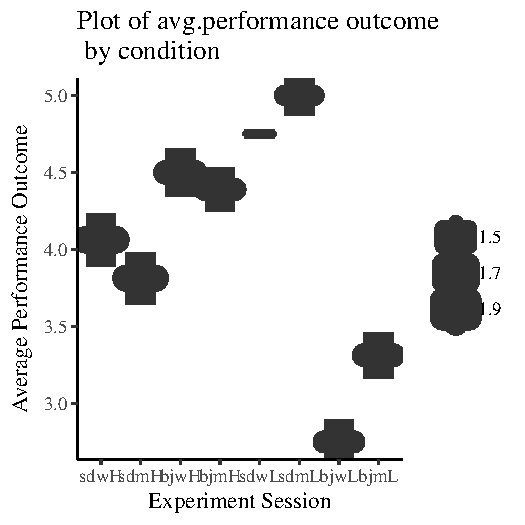
\includegraphics[width=\maxwidth]{/Users/jacob1/Documents/2017/Research/DPhil/Dissertation/finalDocuments/jointActionSocialBonding/images/fullOutcomeAvgSessionBoxplot-1} 

}

\end{figure}


\end{knitrout}




\myparagraph{Prediction 1: More positive perceptions of team performance relative to prior expectations will correlate with higer feelings of team click with the training group}

\begin{knitrout}
\definecolor{shadecolor}{rgb}{0.969, 0.969, 0.969}\color{fgcolor}\begin{kframe}
\begin{alltt}
\hlkwd{library}\hlstd{(tidyverse)}
  \hlstd{groupPerfExpClickScatter} \hlkwb{<-} \hlkwd{ggplot}\hlstd{(twc,} \hlkwd{aes}\hlstd{(}\hlkwc{x}\hlstd{=groupPerformance_3Norm,} \hlkwc{y}\hlstd{=groupClickPostFactor,}
                              \hlkwc{color}\hlstd{=condition))} \hlopt{+} \hlkwd{geom_point}\hlstd{(}\hlkwc{shape} \hlstd{=} \hlnum{1}\hlstd{)} \hlopt{+}
                              \hlkwd{geom_smooth}\hlstd{(}\hlkwc{method}\hlstd{=lm,} \hlkwc{se}\hlstd{=}\hlnum{FALSE}\hlstd{)}   \hlcom{# Don't add shaded confidence region}
  \hlstd{groupPerfExpClickScatter} \hlopt{+}
              \hlkwd{xlab}\hlstd{(}\hlstr{"Group Performance vs Expectations"}\hlstd{)} \hlopt{+}
              \hlkwd{ylab}\hlstd{(}\hlstr{"Group Click"}\hlstd{)} \hlopt{+}
              \hlstd{apatheme}
\end{alltt}


{\ttfamily\noindent\color{warningcolor}{\#\# Warning: Removed 1 rows containing non-finite values (stat\_smooth).}}

{\ttfamily\noindent\color{warningcolor}{\#\# Warning: Removed 1 rows containing missing values (geom\_point).}}\end{kframe}\begin{figure}

{\centering 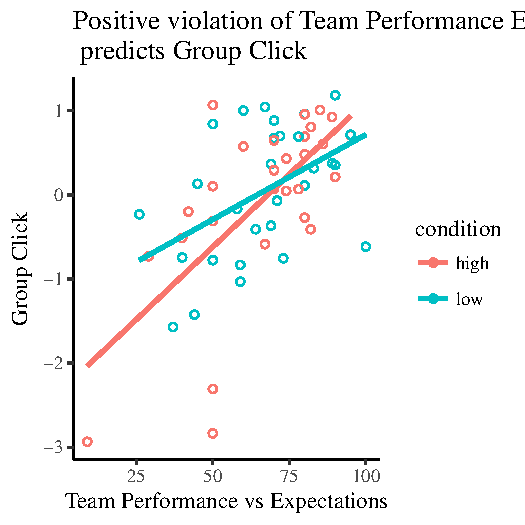
\includegraphics[width=\maxwidth]{/Users/jacob1/Documents/2017/Research/DPhil/Dissertation/finalDocuments/jointActionSocialBonding/images/teamPerfExpClickScatter-1} 

}

\end{figure}


\end{knitrout}



Figure ~\ref{fig:teamPerfExpClickScatter} shows a strong positive correlation between violations of prior expectations concerning team performance and feelings of ``click'' with the training group post-Experiment.  The slope of this relationship appears to vary according to condition, as indicated on the scatterplot by the two non-parallel lines of best fit.

%MODEL:
\begin{knitrout}
\definecolor{shadecolor}{rgb}{0.969, 0.969, 0.969}\color{fgcolor}\begin{kframe}


{\ttfamily\noindent\itshape\color{messagecolor}{\#\# The 'lsmeans' package is being deprecated.\\\#\# Users are encouraged to switch to 'emmeans'.\\\#\# See help('transition') for more information, including how\\\#\# to convert 'lsmeans' objects and scripts to work with 'emmeans'.}}

{\ttfamily\noindent\bfseries\color{errorcolor}{\#\# Error in lsmeans.character.ref.grid(object = new("{}ref.grid"{}, model.info = list(: No variable named groupPerformance\_3Norm in the reference grid}}\end{kframe}
\end{knitrout}

A LMER was used to model the relationship between group performance expectation violations and group click.  Group Performance Expectations, Condition, and their interaction were included as fixed effects, and experiment session was modelled as a random effect (intercept and slope).  To control for perceptions of individual performance relative to prior expectations, post-Experiment arousal, the average performance outcome of each invasion drill trial, and subjective and objective measures of athlete technical competence, these factors were included as fixed effects.

The model revealed a significant positive main effect of group performance expectation violation on feelings of team click with the training group,
  \betavec
    0.3161116
  \CIstart
    0.0587999
  ,
    0.5734233
  \CIfinish
  \SE
    0.1312839
  ,
  t(
    53
    )
  =
    2.4078475
  ,
  \pvalue
    0.0195595
  ,
  \MR
   % groupPerfExpClick.controls.R2[,5]
  ,
  \CR2
   % groupPerfExpClick.controls.R2[,6]
.
The main effect of condition
(
  \betavec
    0.7595177
  \CIstart
    0.1176995
  ,
    1.401336
  \CIfinish
  \SE
    0.3274643,
  t(
    53
  )
  =
    2.3193908
  ,
  \pvalue
    0.0242591
)
and the interaction effect of group performance expectation violation and condition on click
(
  \betavec
    0.4116857
  \CIstart
    0.0737744
  ,
    0.749597
  \CIfinish
  \SE
    0.1724069,
  t(
    53
  )
  =
    2.3878728
  ,
  \pvalue
    0.0205428
)
were also significant.
The average performance outcome of each invasion drill trial was also a significant positive predictor of team click
,
  \betavec
    0.7344113
  \CIstart
    0.2303963
  ,
    1.2384263
  \CIfinish
  \SE
    0.2571552
  ,
  t(
    53
  )
  =
    2.8559063
  ,
  \pvalue
    0.0061153
  (see Table ~\ref{tab:M1lmer})
,
suggesting a relationship between onfield performance and individual athlete perceptions of performance.

These results suggested that group performance expectation violations were a positive predictor of feelings of group click among athletes, and that this relationship was moderated by experiment condition, such that expectation violation had a greater effect on feelings of group click in the high difficulty condition than the low difficulty condition.



%ASSUMPTIONS:
\begin{knitrout}
\definecolor{shadecolor}{rgb}{0.969, 0.969, 0.969}\color{fgcolor}

{\centering 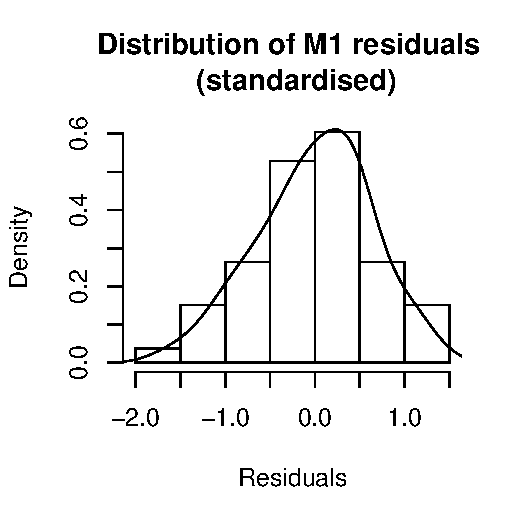
\includegraphics[width=\maxwidth]{/Users/jacob1/Documents/2017/Research/DPhil/Dissertation/finalDocuments/jointActionSocialBonding/images/groupPerfExpClickAssumptionsHist-1} 

}



\end{knitrout}
\begin{knitrout}
\definecolor{shadecolor}{rgb}{0.969, 0.969, 0.969}\color{fgcolor}

{\centering 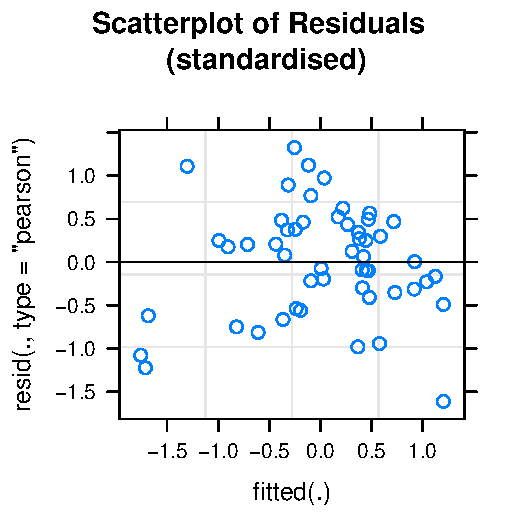
\includegraphics[width=\maxwidth]{/Users/jacob1/Documents/2017/Research/DPhil/Dissertation/finalDocuments/jointActionSocialBonding/images/groupPerfExpClickAssumptionsScatter-1} 

}



\end{knitrout}
\begin{knitrout}
\definecolor{shadecolor}{rgb}{0.969, 0.969, 0.969}\color{fgcolor}

{\centering 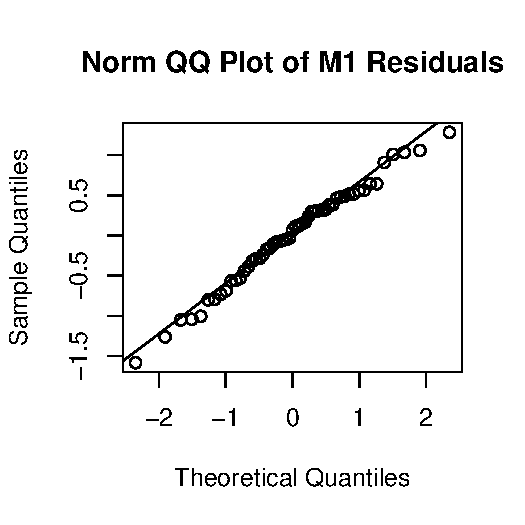
\includegraphics[width=\maxwidth]{/Users/jacob1/Documents/2017/Research/DPhil/Dissertation/finalDocuments/jointActionSocialBonding/images/groupPerfExpClickQQNorm-1} 

}



\end{knitrout}
\begin{knitrout}
\definecolor{shadecolor}{rgb}{0.969, 0.969, 0.969}\color{fgcolor}\begin{kframe}


{\ttfamily\noindent\color{warningcolor}{\#\# Warning in checkConv(attr(opt, "{}derivs"{}), opt\$par, ctrl = control\$checkConv, : unable to evaluate scaled gradient}}

{\ttfamily\noindent\color{warningcolor}{\#\# Warning in checkConv(attr(opt, "{}derivs"{}), opt\$par, ctrl = control\$checkConv, : Model failed to converge: degenerate\ \ Hessian with 1 negative eigenvalues}}

{\ttfamily\noindent\color{warningcolor}{\#\# Warning in checkConv(attr(opt, "{}derivs"{}), opt\$par, ctrl = control\$checkConv, : unable to evaluate scaled gradient}}

{\ttfamily\noindent\color{warningcolor}{\#\# Warning in checkConv(attr(opt, "{}derivs"{}), opt\$par, ctrl = control\$checkConv, : Model failed to converge: degenerate\ \ Hessian with 1 negative eigenvalues}}\end{kframe}

{\centering 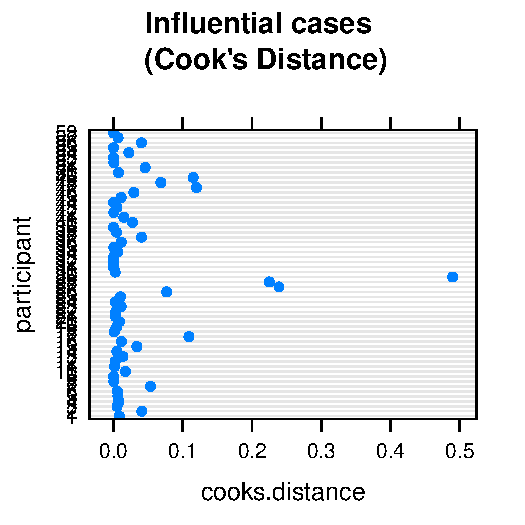
\includegraphics[width=\maxwidth]{/Users/jacob1/Documents/2017/Research/DPhil/Dissertation/finalDocuments/jointActionSocialBonding/images/groupPerfExpClickCooksD-1} 

}



\end{knitrout}

 Model residuals were normally distributed around zero
(
  \resdist
    0.9856688 0.98,
  \pvalue
    0.7721191
)
and an analysis of Cook's distances suggests that the model did not contain any observations that unjustifiably influenced parameter estimates
(all
  \cooksD
    0.55
  ,
  for full presentation of model assumptions, see Appendix Figure ~\ref{fig:M1Assumptions}).

Based on these assessments, the model provided a robust basis for the inference that---in line with predictions---more positive violation of expectations concerning group performance predicted stronger feelings of team click. Also as predicted, this result was moderated by experiment condition, such that the effect of group performance expectation violation on group click was stronger in the high difficulty condition.





\myparagraph{Prediction 1.a: Violations of expectations around team performance moderate the relationship between perceptions of joint action success and team click training group}

\begin{knitrout}
\definecolor{shadecolor}{rgb}{0.969, 0.969, 0.969}\color{fgcolor}\begin{kframe}


{\ttfamily\noindent\itshape\color{messagecolor}{\#\# Saving 3.5 x 3.5 in image}}

{\ttfamily\noindent\color{warningcolor}{\#\# Warning: Removed 1 rows containing missing values (geom\_point).}}

{\ttfamily\noindent\color{warningcolor}{\#\# Warning: Removed 1 rows containing missing values (geom\_point).}}\end{kframe}

{\centering 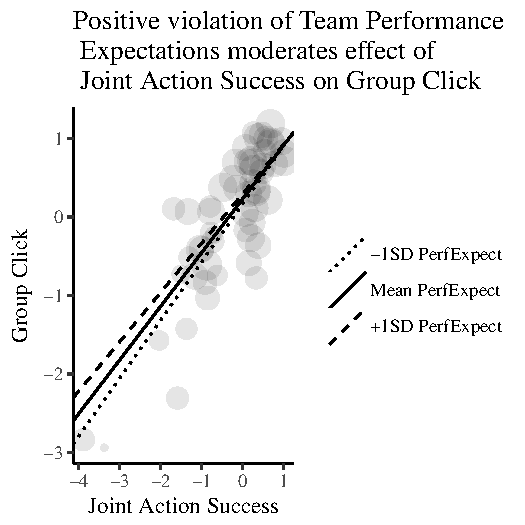
\includegraphics[width=\maxwidth]{/Users/jacob1/Documents/2017/Research/DPhil/Dissertation/finalDocuments/jointActionSocialBonding/images/jASgroupPerfExpClickScatterLM-1} 

}



\end{knitrout}



MODELS








\begin{knitrout}
\definecolor{shadecolor}{rgb}{0.969, 0.969, 0.969}\color{fgcolor}\begin{kframe}


{\ttfamily\noindent\itshape\color{messagecolor}{\#\# Saving 3.5 x 3.5 in image}}

{\ttfamily\noindent\color{warningcolor}{\#\# Warning: Removed 1 rows containing missing values (geom\_point).}}

{\ttfamily\noindent\color{warningcolor}{\#\# Warning: Removed 1 rows containing missing values (geom\_point).}}\end{kframe}

{\centering 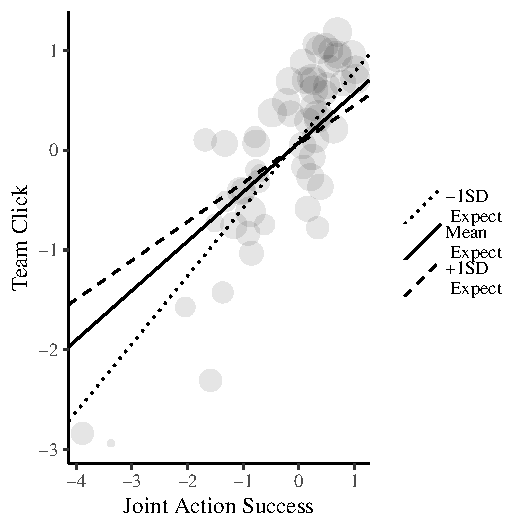
\includegraphics[width=\maxwidth]{/Users/jacob1/Documents/2017/Research/DPhil/Dissertation/finalDocuments/jointActionSocialBonding/images/jASgroupPerfExpClickScatterLMER-1} 

}



\end{knitrout}

Figure ~\ref{fig:teamPerfExpClickScatter} shows that the slope of the relationship between between perceptions of Joint Action Success and Group Click appears to be  moderated by perception of team performance relative to prior expectations, such that higher levels (+1 standard deviation) of group performance expectation violation results in an increase of the steepness of the slope.


A LMER model, with Joint Action Success, Group Performance Expectations, and their interaction included as fixed effects, and perceptions of individual component performance, post-Experiment arousal, and average performance outcome included as controls, confirmed that the negative interation effect of Group Performance Expectations and Joint Action Success on Group Click was significant
,
  \betavec
    -0.2424718
  \CIstart
    -0.3612487
  ,
    -0.123695
  \CIfinish
  \SE
    0.0606015
  ,
  t(
    45.4011883
    )
  =
    -4.0010832
  ,
  \pvalue
    \ensuremath{2.3029093\times 10^{-4}}
  ,
  \MR
   % jASgroupPerfExpClick.int.controls.R2[,5]
  ,
  \CR2
    %jASgroupPerfExpClick.int.controls.R2[,6]
,
suggesting that the relationship between joint action success an group click is more pronounced for \textit{less} positive violations of expectations around group performance.


%%UNUSED MODEL:


%ASSUMPTIONS:
\begin{knitrout}
\definecolor{shadecolor}{rgb}{0.969, 0.969, 0.969}\color{fgcolor}

{\centering 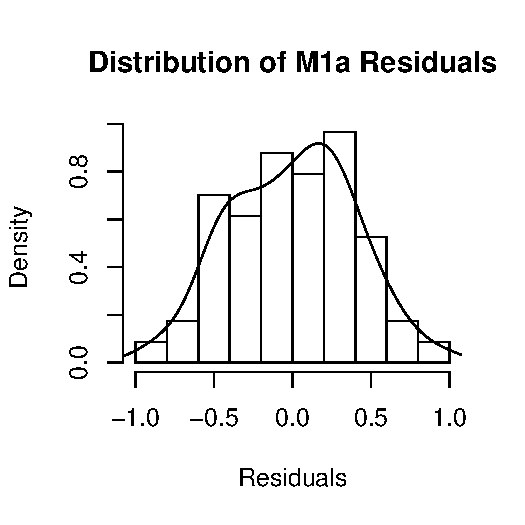
\includegraphics[width=\maxwidth]{/Users/jacob1/Documents/2017/Research/DPhil/Dissertation/finalDocuments/jointActionSocialBonding/images/jASgroupPerfExpClickIntHist-1} 

}



\end{knitrout}
\begin{knitrout}
\definecolor{shadecolor}{rgb}{0.969, 0.969, 0.969}\color{fgcolor}

{\centering 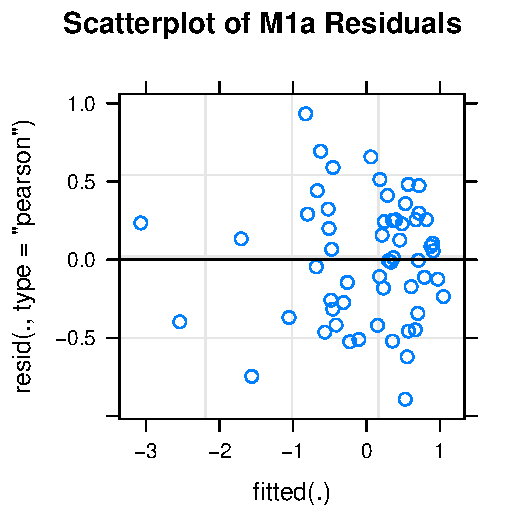
\includegraphics[width=\maxwidth]{/Users/jacob1/Documents/2017/Research/DPhil/Dissertation/finalDocuments/jointActionSocialBonding/images/jASgroupPerfExpClickIntScatter-1} 

}



\end{knitrout}
\begin{knitrout}
\definecolor{shadecolor}{rgb}{0.969, 0.969, 0.969}\color{fgcolor}

{\centering 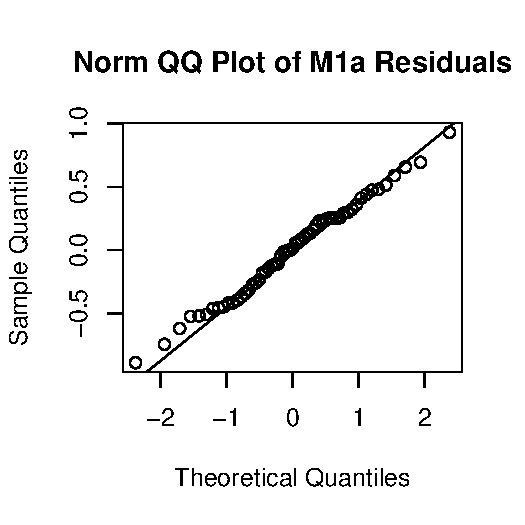
\includegraphics[width=\maxwidth]{/Users/jacob1/Documents/2017/Research/DPhil/Dissertation/finalDocuments/jointActionSocialBonding/images/jASgroupPerfExpClick_int_controlsQQNorm-1} 

}



\end{knitrout}
\begin{knitrout}
\definecolor{shadecolor}{rgb}{0.969, 0.969, 0.969}\color{fgcolor}\begin{kframe}


{\ttfamily\noindent\color{warningcolor}{\#\# Warning in checkConv(attr(opt, "{}derivs"{}), opt\$par, ctrl = control\$checkConv, : unable to evaluate scaled gradient}}

{\ttfamily\noindent\color{warningcolor}{\#\# Warning in checkConv(attr(opt, "{}derivs"{}), opt\$par, ctrl = control\$checkConv, : Model failed to converge: degenerate\ \ Hessian with 1 negative eigenvalues}}

{\ttfamily\noindent\color{warningcolor}{\#\# Warning in checkConv(attr(opt, "{}derivs"{}), opt\$par, ctrl = control\$checkConv, : unable to evaluate scaled gradient}}

{\ttfamily\noindent\color{warningcolor}{\#\# Warning in checkConv(attr(opt, "{}derivs"{}), opt\$par, ctrl = control\$checkConv, : Model failed to converge: degenerate\ \ Hessian with 1 negative eigenvalues}}

{\ttfamily\noindent\color{warningcolor}{\#\# Warning in checkConv(attr(opt, "{}derivs"{}), opt\$par, ctrl = control\$checkConv, : unable to evaluate scaled gradient}}

{\ttfamily\noindent\color{warningcolor}{\#\# Warning in checkConv(attr(opt, "{}derivs"{}), opt\$par, ctrl = control\$checkConv, : Model failed to converge: degenerate\ \ Hessian with 1 negative eigenvalues}}\end{kframe}

{\centering 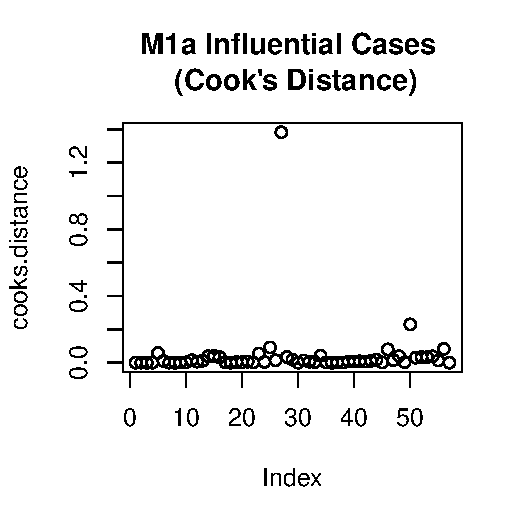
\includegraphics[width=\maxwidth]{/Users/jacob1/Documents/2017/Research/DPhil/Dissertation/finalDocuments/jointActionSocialBonding/images/jASgroupPerfExpClick_intAssumptionsCooksD-1} 

}



\end{knitrout}




Model residuals were normally distributed around zero
(
  \resdist
    0.984615,
  \pvalue
    0.7237464
),
however
an analysis of Cook's distances suggested that the model did contain one influential observation
(
  \cooksD
  =
   2.62,
   see model assumptions in Appendix  ~\ref{fig:M1aAssumptions}
).
Re-running the model with this value excluded led to an improvement of the model fit.
















\myparagraph{Prediction 2: Feelings of group click predict feelings of social bonding to the training group}

\begin{knitrout}
\definecolor{shadecolor}{rgb}{0.969, 0.969, 0.969}\color{fgcolor}\begin{kframe}
\begin{alltt}
  \hlstd{groupClickBondScatter} \hlkwb{<-} \hlkwd{ggplot}\hlstd{(twc,} \hlkwd{aes}\hlstd{(}\hlkwc{x}\hlstd{=groupClickPostFactor,}
                              \hlkwc{y}\hlstd{=groupBondingFactorPost,} \hlkwc{color}\hlstd{=condition))} \hlopt{+} \hlkwd{geom_point}\hlstd{(}\hlkwc{shape} \hlstd{=} \hlnum{1}\hlstd{)} \hlopt{+}
                             \hlkwd{geom_smooth}\hlstd{(}\hlkwc{method}\hlstd{=lm,} \hlkwc{se}\hlstd{=F)}   \hlcom{#  add shaded confidence region}
  \hlstd{groupClickBondScatter} \hlopt{+}
  \hlcom{#              guides(color = guide_legend(title="Condition"))+}
              \hlkwd{theme}\hlstd{(}\hlkwc{plot.title} \hlstd{=} \hlkwd{element_text}\hlstd{(}\hlkwc{size}\hlstd{=}\hlnum{12}\hlstd{))} \hlopt{+}
              \hlkwd{labs}\hlstd{(}\hlkwc{x} \hlstd{=} \hlstr{"Group Click"}\hlstd{,} \hlkwc{y} \hlstd{=} \hlstr{"Social Bonding"}\hlstd{,} \hlkwc{color} \hlstd{=} \hlstr{"Condition"}\hlstd{)}\hlopt{+}
              \hlstd{apatheme} \hlopt{+}
              \hlkwd{ggsave}\hlstd{(}\hlstr{"groupClickBondScatter.pdf"}\hlstd{)}
              \hlcom{#              scale_fill_}
              \hlcom{#"Perceptions of Group Click \textbackslash{}n predict feelings of Social Bonding to training group"}
              \hlcom{#guides(fill=guide_legend("my awesome title"))}
\end{alltt}
\end{kframe}
\end{knitrout}

Figure ~\ref{fig:groupClickBondScatter} shows a clear relationship between Group Click and Social Bonding to the training group following the training group, with the slope for the high difficulty condition appearing slightly steeper than the low difficulty condition.

%%MODEL:


A LMER model (controlling for arousal, average trial performance outcome, and technical competence (subjective and objective)) revealed a strong positive relationship between feelings of group click and feelings of social bonding to the training group,

  \betavec
    0.4323209
  \CIstart
    0.1458563
  ,
    0.7187856
  \CIfinish
  \SE
    0.1461581
  ,
  t(
    29.2159604
    )
  =
    2.957899
  ,
  \pvalue
    0.0060807
  ,
  \MR
   % clickBondingCondition.controls.R2[,5]
  ,
  \CR2
   % clickBondingCondition.controls.R2[,6]
.
The interaction effect of group click and condition on social bonding was not significant
,
  \betavec
    0.2608971
  \CIstart
    -0.0784524
  ,
    0.6002465
  \CIfinish
  \SE
    0.1731407
  ,
  t(
    30.4356925
    )
  =
    1.5068503
  ,
  \pvalue
    0.1421591
,
suggesting that athletes who felt stronger levels of group click also felt stronger levels of social bonding to their training group, irrespective of experiment condition.

%ASSUMPTIONS:
\begin{knitrout}
\definecolor{shadecolor}{rgb}{0.969, 0.969, 0.969}\color{fgcolor}

{\centering 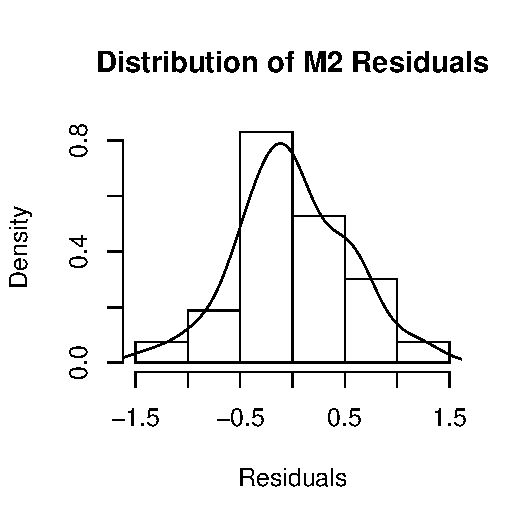
\includegraphics[width=\maxwidth]{/Users/jacob1/Documents/2017/Research/DPhil/Dissertation/finalDocuments/jointActionSocialBonding/images/clickBondingConditionHist-1} 

}



\end{knitrout}
\begin{knitrout}
\definecolor{shadecolor}{rgb}{0.969, 0.969, 0.969}\color{fgcolor}

{\centering 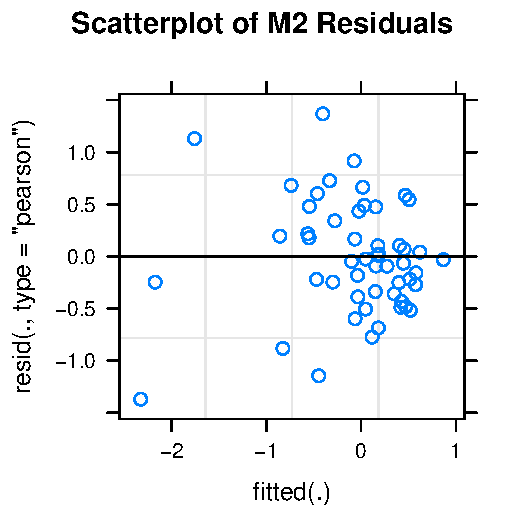
\includegraphics[width=\maxwidth]{/Users/jacob1/Documents/2017/Research/DPhil/Dissertation/finalDocuments/jointActionSocialBonding/images/clickBondingConditionScatter-1} 

}



\end{knitrout}
\begin{knitrout}
\definecolor{shadecolor}{rgb}{0.969, 0.969, 0.969}\color{fgcolor}

{\centering 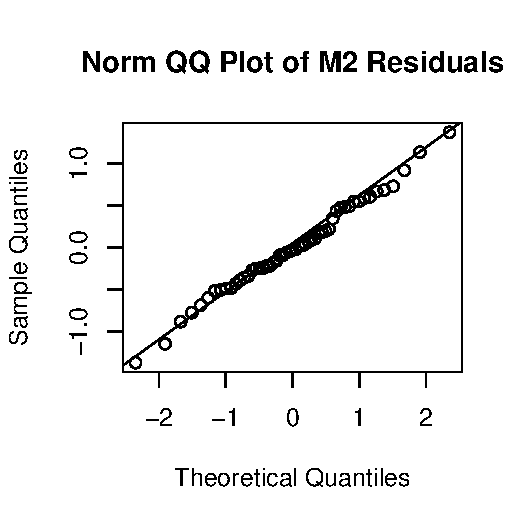
\includegraphics[width=\maxwidth]{/Users/jacob1/Documents/2017/Research/DPhil/Dissertation/finalDocuments/jointActionSocialBonding/images/clickBondingConditionQQNorm-1} 

}



\end{knitrout}
\begin{knitrout}
\definecolor{shadecolor}{rgb}{0.969, 0.969, 0.969}\color{fgcolor}\begin{kframe}


{\ttfamily\noindent\color{warningcolor}{\#\# Warning in checkConv(attr(opt, "{}derivs"{}), opt\$par, ctrl = control\$checkConv, : unable to evaluate scaled gradient}}

{\ttfamily\noindent\color{warningcolor}{\#\# Warning in checkConv(attr(opt, "{}derivs"{}), opt\$par, ctrl = control\$checkConv, : Model failed to converge: degenerate\ \ Hessian with 1 negative eigenvalues}}\end{kframe}

{\centering 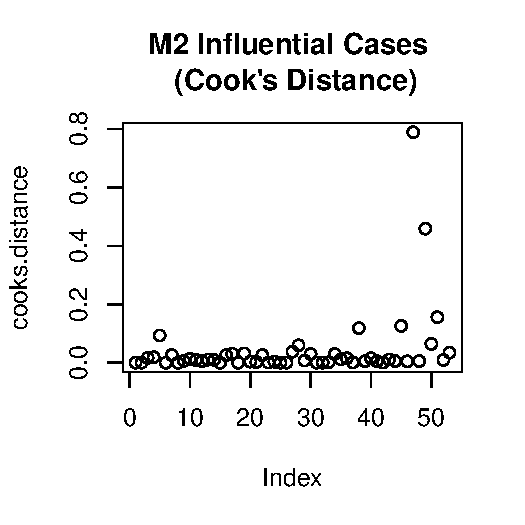
\includegraphics[width=\maxwidth]{/Users/jacob1/Documents/2017/Research/DPhil/Dissertation/finalDocuments/jointActionSocialBonding/images/clickBondingConditionCooksD-1} 

}



\end{knitrout}

Model residuals were normally distributed around zero
(
  \resdist
    0.9879743,
  \pvalue
    0.8688934
)
and there were no unjustifiably influential cases
(
all
\cooksD
  0.66, see model assumptions in Appendix  ~\ref{fig:M2Assumptions}
)
.
These results suggested that feelings of group click were a powerful predictor of feelings of social bonding in the study sample.








\myparagraph{Prediction 3: More positive perceptions of team performance relative to expectations will predict higher levels of Social Bonding to the training group}


\begin{knitrout}
\definecolor{shadecolor}{rgb}{0.969, 0.969, 0.969}\color{fgcolor}\begin{kframe}


{\ttfamily\noindent\itshape\color{messagecolor}{\#\# Saving 3.5 x 3.5 in image}}

{\ttfamily\noindent\color{warningcolor}{\#\# Warning: Removed 1 rows containing non-finite values (stat\_smooth).}}

{\ttfamily\noindent\color{warningcolor}{\#\# Warning: Removed 1 rows containing missing values (geom\_point).}}

{\ttfamily\noindent\color{warningcolor}{\#\# Warning: Removed 1 rows containing non-finite values (stat\_smooth).}}

{\ttfamily\noindent\color{warningcolor}{\#\# Warning: Removed 1 rows containing missing values (geom\_point).}}\end{kframe}\begin{figure}

{\centering 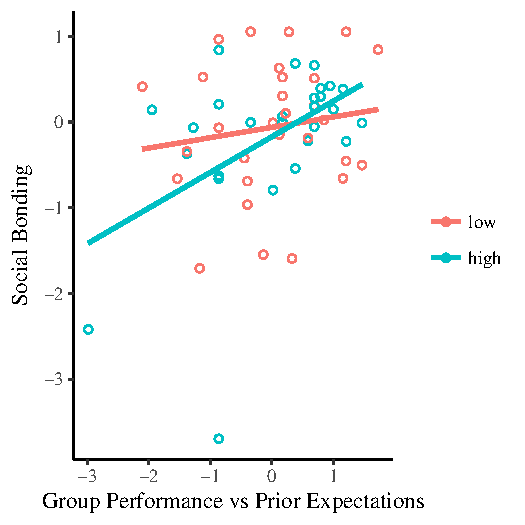
\includegraphics[width=\maxwidth]{/Users/jacob1/Documents/2017/Research/DPhil/Dissertation/finalDocuments/jointActionSocialBonding/images/groupPerfExpBondConditionScatter-1} 

}

\caption[Positive violation of group performance expectations 
 predict feelings of Social Bonding to training group]{Positive violation of group performance expectations 
 predict feelings of Social Bonding to training group}\label{fig:groupPerfExpBondConditionScatter}
\end{figure}


\end{knitrout}

  %<<groupPerfExpBondScatter1, fig.cap=''>>=
  %  teamPerfExpBondScatter1 <- ggplot(twc, aes(x=groupPerformance_3Norm, y=groupBondingFactorPost)) + geom_point(shape = 1) +
  %                              geom_smooth(method=lm, se=FALSE)
  %  teamPerfExpBondScatter1 +
  %              ggtitle("Perceptions of Team Performance (vs prior expectations) \n %              theme(plot.title = element_text(size=12)) +
  %              xlab("Team Performance vs Prior Expectations") +
  %              ylab("Social Bonding") +
  %              apatheme
  %@
@
Figure ~\ref{fig:groupPerfExpBondConditionScatter} shows a positive relationship between violation of group performance expectations and Social Bonding to the training group.  The plot shows a pronounced difference in the slope of each experimental condition, suggesting that the relationship was stronger in the high difficulty condition.

%%MODEL:

A LMER model with group performance expectation violation, condition, and their interaction as fixed effects, experiment session as random effect (correlated slope and intercept), and controls, revealed a significant positive relationship between the interaction of group performance expectation violation and condition on social bonding
  ,
  \betavec
    0.4590893
  \CIstart
    0.0990681
  ,
    0.8191105
  \CIfinish
  \SE
    0.1836877
  ,
  t(
    53
    )
  =
    2.4992931
  ,
  \pvalue
    0.0155768
  ,
  \MR
   % groupPerfExpBondingCondition.controls.R2[,5]
  ,
  \CR2
   % groupPerfExpBondingCondition.controls.R2[,6]
  .
The main effects of group performance expectation violation
(
  \betavec
    0.0077975
  \CIstart
    -0.2663504
  ,
    0.2819454
  \CIfinish
  \SE
    0.139874
  ,
  t(
    53
    )
  =
    0.0557466
  ,
  \pvalue
    0.9557533
  )
  and experiment condition
  (
  \betavec
    0.5615116
  \CIstart
    -0.1223016
  ,
    1.2453248
  \CIfinish
  \SE
    0.3488907
  ,
  t(
    53
    )
  =
    1.6094197
  ,
  \pvalue
    0.1134656
)
were not significant predictors of social bonding.  Average performance in each trial was, however, a significant predictor of social bonding
,
  \betavec
    0.64863
  \CIstart
    0.1116367
  ,
    1.1856233
  \CIfinish
  \SE
    0.2739812
  ,
  t(
    53
    )
  =
    2.3674251
  ,
  \pvalue
    0.0215951
.

%ASSUMPTIONS:
\begin{knitrout}
\definecolor{shadecolor}{rgb}{0.969, 0.969, 0.969}\color{fgcolor}

{\centering 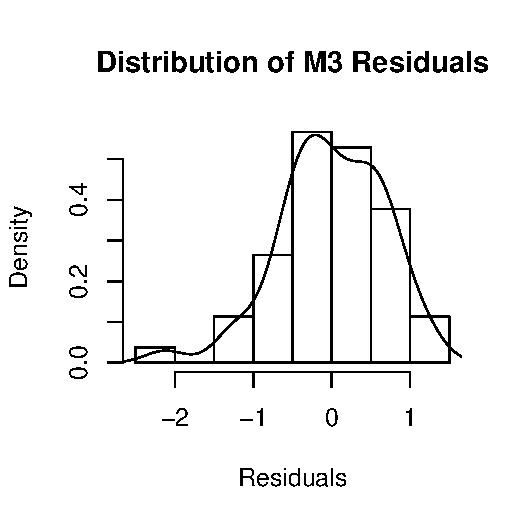
\includegraphics[width=\maxwidth]{/Users/jacob1/Documents/2017/Research/DPhil/Dissertation/finalDocuments/jointActionSocialBonding/images/groupPerfExpBondingConditionHist-1} 

}



\end{knitrout}
\begin{knitrout}
\definecolor{shadecolor}{rgb}{0.969, 0.969, 0.969}\color{fgcolor}

{\centering 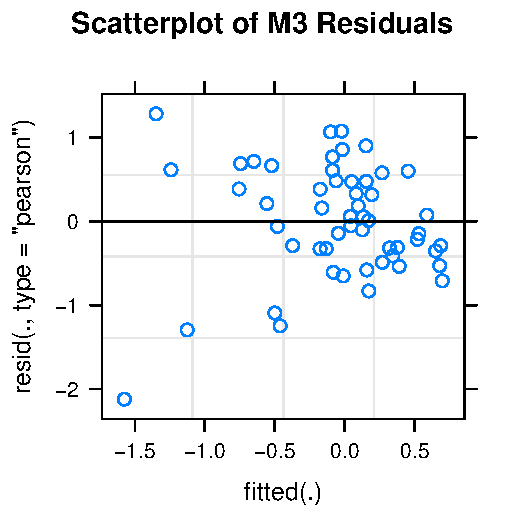
\includegraphics[width=\maxwidth]{/Users/jacob1/Documents/2017/Research/DPhil/Dissertation/finalDocuments/jointActionSocialBonding/images/groupPerfExpBondingConditionScatter-1} 

}



\end{knitrout}
\begin{knitrout}
\definecolor{shadecolor}{rgb}{0.969, 0.969, 0.969}\color{fgcolor}

{\centering 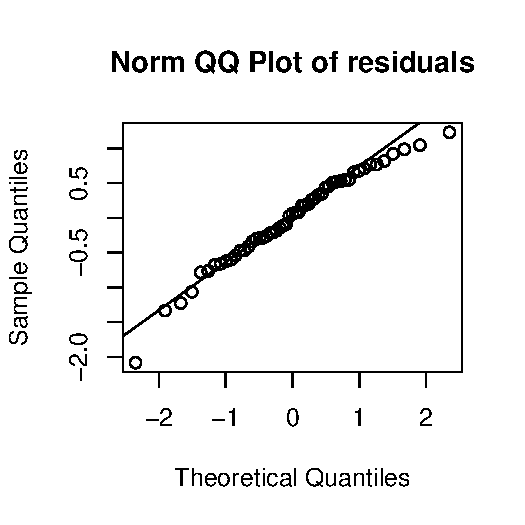
\includegraphics[width=\maxwidth]{/Users/jacob1/Documents/2017/Research/DPhil/Dissertation/finalDocuments/jointActionSocialBonding/images/groupPerfExpBondingConditionQQNorm-1} 

}



\end{knitrout}
\begin{knitrout}
\definecolor{shadecolor}{rgb}{0.969, 0.969, 0.969}\color{fgcolor}\begin{kframe}


{\ttfamily\noindent\color{warningcolor}{\#\# Warning in optwrap(optimizer, devfun, getStart(start, rho\$lower, rho\$pp), : convergence code 1 from optimx}}

{\ttfamily\noindent\color{warningcolor}{\#\# Warning in optwrap(optimizer, devfun, getStart(start, rho\$lower, rho\$pp), : convergence code 1 from optimx}}\end{kframe}

{\centering 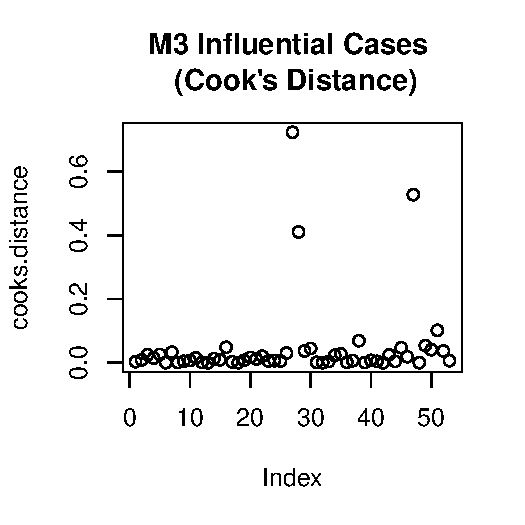
\includegraphics[width=\maxwidth]{/Users/jacob1/Documents/2017/Research/DPhil/Dissertation/finalDocuments/jointActionSocialBonding/images/groupPerfExpBondingConditionCooksD-1} 

}



\end{knitrout}

Model residuals were normally distributed around zero
(
  \resdist
    0.984615,
  \pvalue
    0.7237464
)
and all \cooksD were less than
  0.55
(
see model assumptions in Appendix  ~\ref{fig:M1aAssumptions}
)
.

These results suggested that the relationship between positive violation of group performance expectations and social bonding was significant, only in the high difficulty condition, and not overall accoss conditions.


\myparagraph{Prediction 4: Feelings of group click will mediate a relationship between more positive perceptions of team performance relative to prior expectations around group performance and social bonding to the group}




\begin{knitrout}
\definecolor{shadecolor}{rgb}{0.969, 0.969, 0.969}\color{fgcolor}\begin{kframe}


{\ttfamily\noindent\bfseries\color{errorcolor}{\#\# Error in plot(med.out.groupPerfExp, main = "{}Mediation Model"{}): object 'med.out.groupPerfExp' not found}}\end{kframe}
\end{knitrout}


\begin{knitrout}
\definecolor{shadecolor}{rgb}{0.969, 0.969, 0.969}\color{fgcolor}\begin{kframe}


{\ttfamily\noindent\bfseries\color{errorcolor}{\#\# Error in mediate(m2, m3, treat = "{}groupPerformance\_3Norm"{}, mediator = "{}groupClickPostFactor"{}): unused arguments (treat = "{}groupPerformance\_3Norm"{}, mediator = "{}groupClickPostFactor"{})}}

{\ttfamily\noindent\bfseries\color{errorcolor}{\#\# Error in summary(med.out.postExperiment): object 'med.out.postExperiment' not found}}

{\ttfamily\noindent\bfseries\color{errorcolor}{\#\# Error in mediate(m2, m3, treat = "{}groupPerformance\_3Norm"{}, mediator = "{}groupClickPostFactor"{}, : unused arguments (treat = "{}groupPerformance\_3Norm"{}, mediator = "{}groupClickPostFactor"{}, covariates = list(condition = "{}high"{}))}}

{\ttfamily\noindent\bfseries\color{errorcolor}{\#\# Error in summary(med.out.postExperiment.High): object 'med.out.postExperiment.High' not found}}

{\ttfamily\noindent\bfseries\color{errorcolor}{\#\# Error in mediate(m2, m3, treat = "{}groupPerformance\_3Norm"{}, mediator = "{}groupClickPostFactor"{}, : unused arguments (treat = "{}groupPerformance\_3Norm"{}, mediator = "{}groupClickPostFactor"{}, covariates = list(condition = "{}low"{}))}}

{\ttfamily\noindent\bfseries\color{errorcolor}{\#\# Error in summary(med.out.postExperiment.Low): object 'med.out.postExperiment.Low' not found}}\end{kframe}
\end{knitrout}













Mediation analyses were conducted using linear mixed effects regressions in the Causal Mediation Analysis package in R (Version 4.4.5).  To make inferences concerning the average indirect and total effects, quasi-Bayesian Markov Chain Monte Carlo (MCMC) method based on normal approximation and 1000 simulations was used to estimate the 95\% Confidence Intervals \citep{Tofighi2016a,Imai2010}. MCMC estimation is a form of non-parametric bootstrapping whereby the sampling distribution for the effect of interest is not assumed to be normal but is instead simulated from the model estimates and their asymptotic variances and covariances \cite{Preacher2008}.

Results of the mediation analysis revealed significant average indirect effect of Group Performance Expectation Violation on Social Bonding attributable to Team Click,
  \betavec
   % coef(summary(med.out.groupPerfExp))["ACME (average)", "Estimate"]
  \CIstart
   % coef(summary(med.out.groupPerfExp))["ACME (average)","95% CI Lower"]
  ,
   % coef(summary(med.out.groupPerfExp))["ACME (average)","95% CI Upper"]
  \CIfinish
  ,
  \pvalue
   % coef(summary(med.out.groupPerfExp))["ACME (average)","p-value"]
  ,
  .
When controlling for the effect of team click on social bonding, the average direct effect between Joint Action Success and Social Bonding was no longer significant, \Sexpr{} (see Figure ~\ref{fig:groupPerfExpClickMediationPlot}).  These results suggest that feelings of team click fully mediate the relationship between group performance expectation violation and and social bonding.




\myparagraph{Discussion of post-Experiment results}























\end{document}







\subsubsection{Analysis of pre- and post-Experiment survey data}


%%%%%%%%%%%%%%%%%%%%%%%%%%%%%%%%%%%%%%%%%%%%%%%%%%%%%%%%%%%%%%%%%%%%%%%%%%%%%%%%%%%%%%%
PRE-POST ANALYSIS:
%%%%%%%%%%%%%%%%%%%%%%%%%%%%%%%%%
1. pre-post changes:
  i. performance expectations?
  ii. click?
  iii. bonding?



\begin{knitrout}
\definecolor{shadecolor}{rgb}{0.969, 0.969, 0.969}\color{fgcolor}\begin{kframe}


{\ttfamily\noindent\color{warningcolor}{\#\# Warning in min(x): no non-missing arguments to min; returning Inf}}

{\ttfamily\noindent\color{warningcolor}{\#\# Warning in max(x): no non-missing arguments to max; returning -Inf}}\end{kframe}
\end{knitrout}









\begin{knitrout}
\definecolor{shadecolor}{rgb}{0.969, 0.969, 0.969}\color{fgcolor}\begin{kframe}


{\ttfamily\noindent\itshape\color{messagecolor}{\#\# Saving 3.5 x 3.5 in image}}

{\ttfamily\noindent\color{warningcolor}{\#\# Warning: Removed 59 rows containing non-finite values (stat\_boxplot).}}

{\ttfamily\noindent\color{warningcolor}{\#\# Warning: Removed 59 rows containing non-finite values (stat\_boxplot).}}\end{kframe}

{\centering 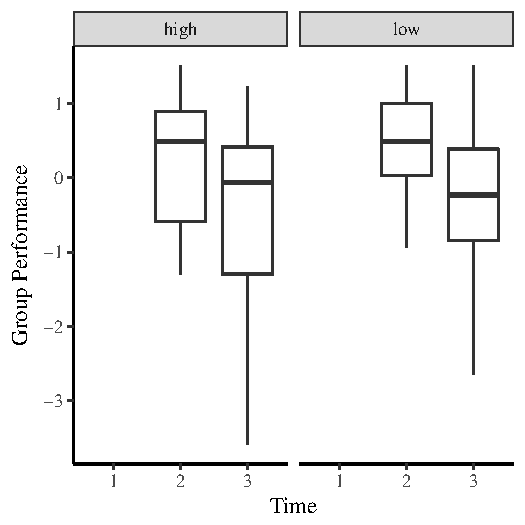
\includegraphics[width=\maxwidth]{/Users/jacob1/Documents/2017/Research/DPhil/Dissertation/finalDocuments/jointActionSocialBonding/images/groupPerfConfPlot-1} 

}



\end{knitrout}







\begin{knitrout}
\definecolor{shadecolor}{rgb}{0.969, 0.969, 0.969}\color{fgcolor}\begin{kframe}


{\ttfamily\noindent\itshape\color{messagecolor}{\#\# Saving 3.5 x 3.5 in image}}

{\ttfamily\noindent\color{warningcolor}{\#\# Warning: Removed 59 rows containing non-finite values (stat\_boxplot).}}

{\ttfamily\noindent\color{warningcolor}{\#\# Warning: Removed 59 rows containing non-finite values (stat\_boxplot).}}\end{kframe}\begin{figure}

{\centering 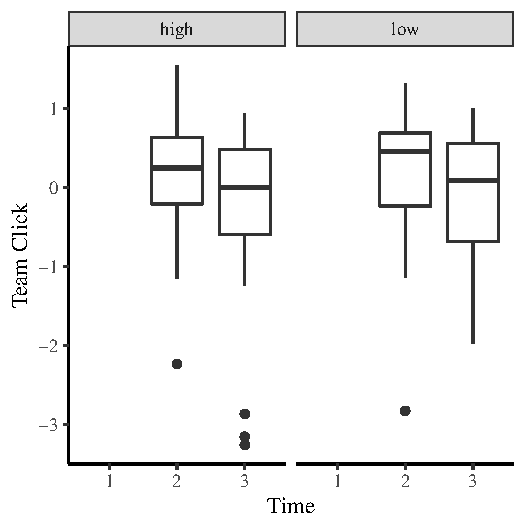
\includegraphics[width=\maxwidth]{/Users/jacob1/Documents/2017/Research/DPhil/Dissertation/finalDocuments/jointActionSocialBonding/images/prePostClickPlot-1} 

}

\caption[Pre- and post-Experiment measures of group click]{Pre- and post-Experiment measures of group click}\label{fig:prePostClickPlot}
\end{figure}


\end{knitrout}





\begin{knitrout}
\definecolor{shadecolor}{rgb}{0.969, 0.969, 0.969}\color{fgcolor}\begin{kframe}


{\ttfamily\noindent\itshape\color{messagecolor}{\#\# Saving 3.5 x 3.5 in image}}

{\ttfamily\noindent\color{warningcolor}{\#\# Warning: Removed 59 rows containing non-finite values (stat\_boxplot).}}

{\ttfamily\noindent\color{warningcolor}{\#\# Warning: Removed 59 rows containing non-finite values (stat\_boxplot).}}\end{kframe}\begin{figure}

{\centering 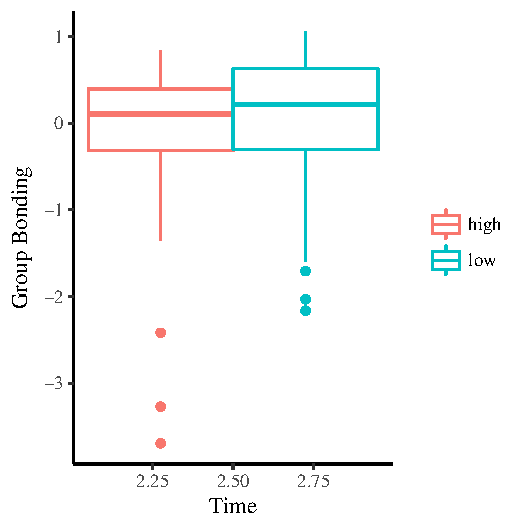
\includegraphics[width=\maxwidth]{/Users/jacob1/Documents/2017/Research/DPhil/Dissertation/finalDocuments/jointActionSocialBonding/images/prePostBondingPlot-1} 

}

\caption[Pre- and post-Experiment measures of group Bonding]{Pre- and post-Experiment measures of group Bonding}\label{fig:prePostBondingPlot}
\end{figure}


\end{knitrout}










\begin{knitrout}
\definecolor{shadecolor}{rgb}{0.969, 0.969, 0.969}\color{fgcolor}

{\centering 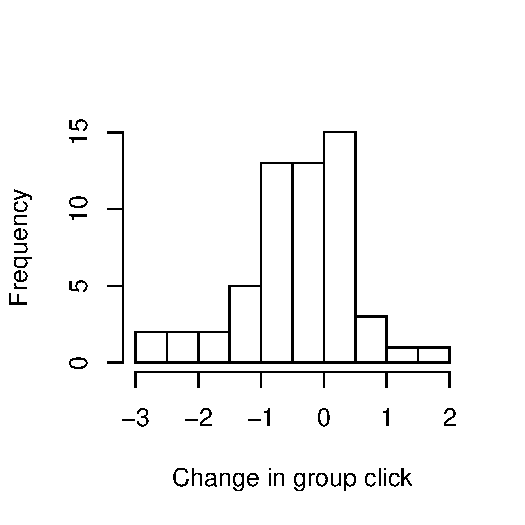
\includegraphics[width=\maxwidth]{/Users/jacob1/Documents/2017/Research/DPhil/Dissertation/finalDocuments/jointActionSocialBonding/images/prePostVariables-1} 

}




{\centering 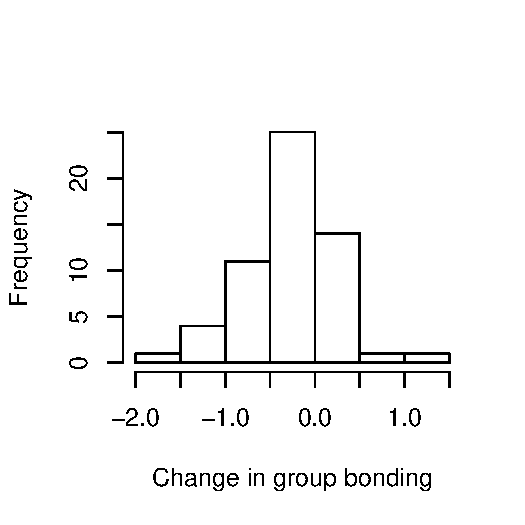
\includegraphics[width=\maxwidth]{/Users/jacob1/Documents/2017/Research/DPhil/Dissertation/finalDocuments/jointActionSocialBonding/images/prePostVariables-2} 

}




{\centering 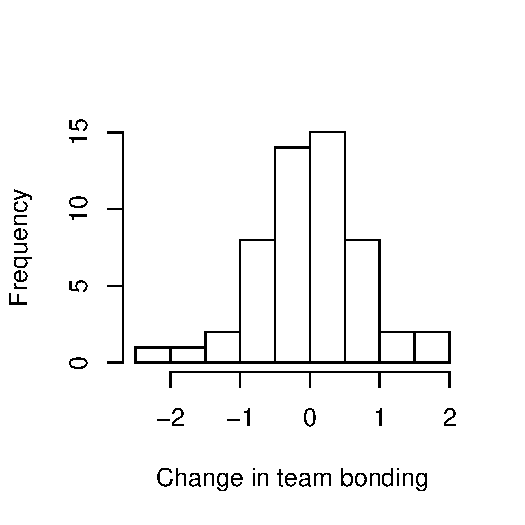
\includegraphics[width=\maxwidth]{/Users/jacob1/Documents/2017/Research/DPhil/Dissertation/finalDocuments/jointActionSocialBonding/images/prePostVariables-3} 

}




{\centering 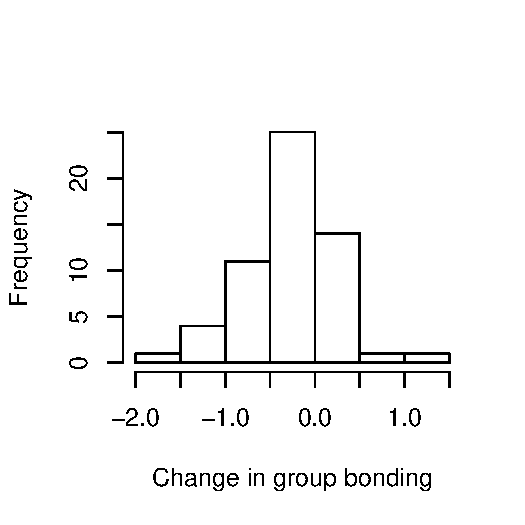
\includegraphics[width=\maxwidth]{/Users/jacob1/Documents/2017/Research/DPhil/Dissertation/finalDocuments/jointActionSocialBonding/images/prePostVariables-4} 

}




{\centering 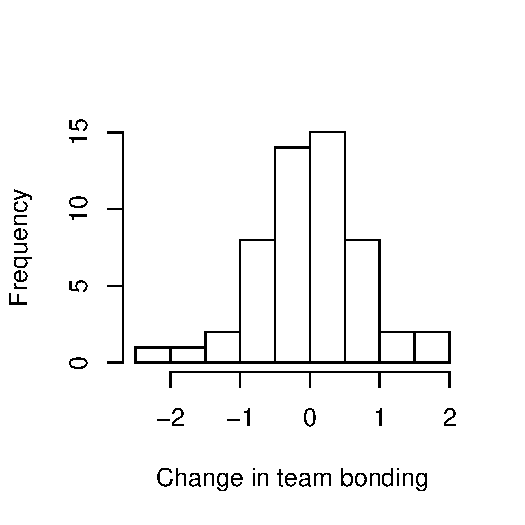
\includegraphics[width=\maxwidth]{/Users/jacob1/Documents/2017/Research/DPhil/Dissertation/finalDocuments/jointActionSocialBonding/images/prePostVariables-5} 

}



\end{knitrout}

\begin{knitrout}
\definecolor{shadecolor}{rgb}{0.969, 0.969, 0.969}\color{fgcolor}

{\centering 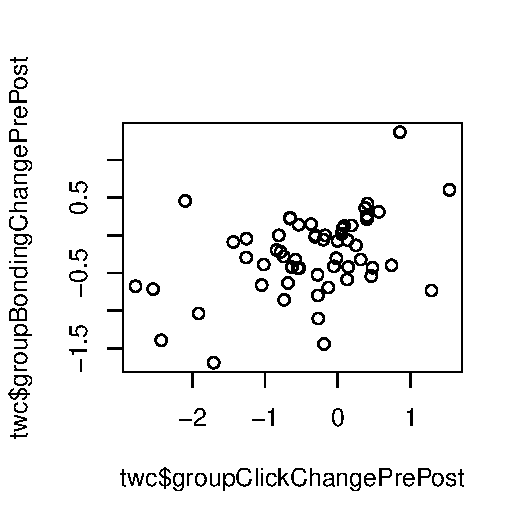
\includegraphics[width=\maxwidth]{/Users/jacob1/Documents/2017/Research/DPhil/Dissertation/finalDocuments/jointActionSocialBonding/images/exploreRelationshipsPrePost-1} 

}




{\centering 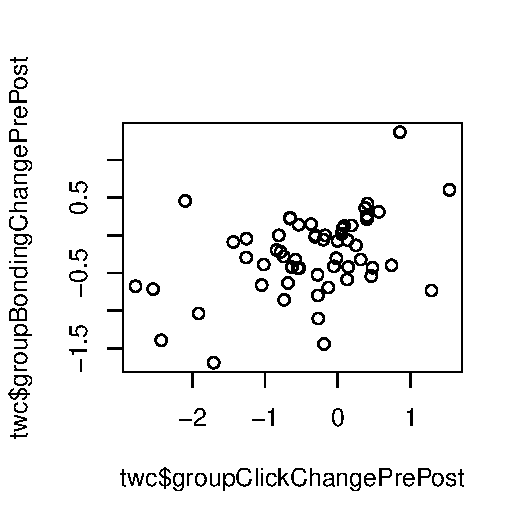
\includegraphics[width=\maxwidth]{/Users/jacob1/Documents/2017/Research/DPhil/Dissertation/finalDocuments/jointActionSocialBonding/images/exploreRelationshipsPrePost-2} 

}




{\centering \includegraphics[width=\maxwidth]{/Users/jacob1/Documents/2017/Research/DPhil/Dissertation/finalDocuments/jointActionSocialBonding/images/exploreRelationshipsPrePost-3} 

}



\end{knitrout}





\begin{knitrout}
\definecolor{shadecolor}{rgb}{0.969, 0.969, 0.969}\color{fgcolor}\begin{kframe}


{\ttfamily\noindent\color{warningcolor}{\#\# Warning in ICCest(sessionName, groupPerfChangePrePostNorm, data = twc, CI.type = "{}THD"{}):}}

{\ttfamily\noindent\color{warningcolor}{\#\# Warning in ICCest(sessionName, groupClickChangePrePostNorm, data = twc, :}}

{\ttfamily\noindent\color{warningcolor}{\#\# Warning in ICCest(sessionName, groupBondingChangePrePostNorm, data = twc, :}}

{\ttfamily\noindent\color{warningcolor}{\#\# Warning in ICCest(sessionName, teamBondingChangePrePostNorm, data = twc, :}}\end{kframe}
\end{knitrout}


\begin{knitrout}
\definecolor{shadecolor}{rgb}{0.969, 0.969, 0.969}\color{fgcolor}\begin{kframe}


{\ttfamily\noindent\color{warningcolor}{\#\# Warning in ICCest(sex, groupPerfChangePrePostNorm, data = twc, CI.type = "{}THD"{}):}}

{\ttfamily\noindent\color{warningcolor}{\#\# Warning in ICCest(sex, groupClickChangePrePostNorm, data = twc, CI.type = "{}THD"{}):}}

{\ttfamily\noindent\color{warningcolor}{\#\# Warning in ICCest(sex, groupBondingChangePrePostNorm, data = twc, CI.type = "{}THD"{}):}}

{\ttfamily\noindent\color{warningcolor}{\#\# Warning in ICCest(sex, teamBondingChangePrePostNorm, data = twc, CI.type = "{}THD"{}):}}\end{kframe}
\end{knitrout}

\begin{knitrout}
\definecolor{shadecolor}{rgb}{0.969, 0.969, 0.969}\color{fgcolor}\begin{kframe}


{\ttfamily\noindent\color{warningcolor}{\#\# Warning in ICCest(team, groupPerfChangePrePostNorm, data = twc, CI.type = "{}THD"{}):}}

{\ttfamily\noindent\color{warningcolor}{\#\# Warning in ICCest(team, groupClickChangePrePostNorm, data = twc, CI.type = "{}THD"{}):}}

{\ttfamily\noindent\color{warningcolor}{\#\# Warning in ICCest(team, groupBondingChangePrePostNorm, data = twc, CI.type = "{}THD"{}):}}

{\ttfamily\noindent\color{warningcolor}{\#\# Warning in ICCest(team, teamBondingChangePrePostNorm, data = twc, CI.type = "{}THD"{}):}}\end{kframe}
\end{knitrout}

\begin{knitrout}
\definecolor{shadecolor}{rgb}{0.969, 0.969, 0.969}\color{fgcolor}\begin{kframe}


{\ttfamily\noindent\color{warningcolor}{\#\# Warning in ICCest(sessionLocation, groupPerfChangePrePostNorm, data = twc, :}}

{\ttfamily\noindent\color{warningcolor}{\#\# Warning in ICCest(sessionLocation, groupClickChangePrePostNorm, data = twc, :}}

{\ttfamily\noindent\color{warningcolor}{\#\# Warning in ICCest(sessionLocation, groupBondingChangePrePostNorm, data = twc, :}}

{\ttfamily\noindent\color{warningcolor}{\#\# Warning in ICCest(sessionLocation, teamBondingChangePrePostNorm, data = twc, :}}\end{kframe}
\end{knitrout}


\begin{knitrout}
\definecolor{shadecolor}{rgb}{0.969, 0.969, 0.969}\color{fgcolor}\begin{kframe}


{\ttfamily\noindent\itshape\color{messagecolor}{\#\# Saving 3.5 x 3.5 in image}}

{\ttfamily\noindent\color{warningcolor}{\#\# Warning: Removed 1 rows containing non-finite values (stat\_smooth).}}

{\ttfamily\noindent\color{warningcolor}{\#\# Warning: Removed 1 rows containing missing values (geom\_point).}}

{\ttfamily\noindent\color{warningcolor}{\#\# Warning: Removed 1 rows containing non-finite values (stat\_smooth).}}

{\ttfamily\noindent\color{warningcolor}{\#\# Warning: Removed 1 rows containing missing values (geom\_point).}}\end{kframe}

{\centering \includegraphics[width=\maxwidth]{/Users/jacob1/Documents/2017/Research/DPhil/Dissertation/finalDocuments/jointActionSocialBonding/images/groupPerfClickChangeCondition-1} 

}



\end{knitrout}


\begin{knitrout}
\definecolor{shadecolor}{rgb}{0.969, 0.969, 0.969}\color{fgcolor}\begin{kframe}


{\ttfamily\noindent\itshape\color{messagecolor}{\#\# \\\#\# Attaching package: 'lmerTest'}}

{\ttfamily\noindent\itshape\color{messagecolor}{\#\# The following object is masked from 'package:lme4':\\\#\# \\\#\#\ \ \ \  lmer}}

{\ttfamily\noindent\itshape\color{messagecolor}{\#\# The following object is masked from 'package:stats':\\\#\# \\\#\#\ \ \ \  step}}\end{kframe}
\end{knitrout}




%ASSUMPTIONS:
\begin{knitrout}
\definecolor{shadecolor}{rgb}{0.969, 0.969, 0.969}\color{fgcolor}

{\centering \includegraphics[width=\maxwidth]{/Users/jacob1/Documents/2017/Research/DPhil/Dissertation/finalDocuments/jointActionSocialBonding/images/groupPerfClickChangeAssumptionsHist-1} 

}



\end{knitrout}
\begin{knitrout}
\definecolor{shadecolor}{rgb}{0.969, 0.969, 0.969}\color{fgcolor}

{\centering \includegraphics[width=\maxwidth]{/Users/jacob1/Documents/2017/Research/DPhil/Dissertation/finalDocuments/jointActionSocialBonding/images/groupPerfClickChangeAssumptionsScatter-1} 

}



\end{knitrout}
\begin{knitrout}
\definecolor{shadecolor}{rgb}{0.969, 0.969, 0.969}\color{fgcolor}

{\centering \includegraphics[width=\maxwidth]{/Users/jacob1/Documents/2017/Research/DPhil/Dissertation/finalDocuments/jointActionSocialBonding/images/groupPerfClickChangeQQNorm-1} 

}



\end{knitrout}
\begin{knitrout}
\definecolor{shadecolor}{rgb}{0.969, 0.969, 0.969}\color{fgcolor}\begin{kframe}


{\ttfamily\noindent\color{warningcolor}{\#\# Warning in optwrap(optimizer, devfun, getStart(start, rho\$lower, rho\$pp), : convergence code 1 from optimx}}

{\ttfamily\noindent\color{warningcolor}{\#\# Warning in optwrap(optimizer, devfun, getStart(start, rho\$lower, rho\$pp), : convergence code 1 from optimx}}

{\ttfamily\noindent\color{warningcolor}{\#\# Warning in optwrap(optimizer, devfun, getStart(start, rho\$lower, rho\$pp), : convergence code 1 from optimx}}

{\ttfamily\noindent\color{warningcolor}{\#\# Warning in optwrap(optimizer, devfun, getStart(start, rho\$lower, rho\$pp), : convergence code 1 from optimx}}

{\ttfamily\noindent\color{warningcolor}{\#\# Warning in optwrap(optimizer, devfun, getStart(start, rho\$lower, rho\$pp), : convergence code 1 from optimx}}

{\ttfamily\noindent\color{warningcolor}{\#\# Warning in optwrap(optimizer, devfun, getStart(start, rho\$lower, rho\$pp), : convergence code 1 from optimx}}

{\ttfamily\noindent\color{warningcolor}{\#\# Warning in optwrap(optimizer, devfun, getStart(start, rho\$lower, rho\$pp), : convergence code 1 from optimx}}

{\ttfamily\noindent\color{warningcolor}{\#\# Warning in optwrap(optimizer, devfun, getStart(start, rho\$lower, rho\$pp), : convergence code 1 from optimx}}

{\ttfamily\noindent\color{warningcolor}{\#\# Warning in optwrap(optimizer, devfun, getStart(start, rho\$lower, rho\$pp), : convergence code 1 from optimx}}

{\ttfamily\noindent\color{warningcolor}{\#\# Warning in optwrap(optimizer, devfun, getStart(start, rho\$lower, rho\$pp), : convergence code 1 from optimx}}

{\ttfamily\noindent\color{warningcolor}{\#\# Warning in optwrap(optimizer, devfun, opt\$par, lower = rho\$lower, control = control, : convergence code 1 from optimx}}

{\ttfamily\noindent\color{warningcolor}{\#\# Warning in optwrap(optimizer, devfun, getStart(start, rho\$lower, rho\$pp), : convergence code 1 from optimx}}

{\ttfamily\noindent\color{warningcolor}{\#\# Warning in optwrap(optimizer, devfun, getStart(start, rho\$lower, rho\$pp), : convergence code 1 from optimx}}

{\ttfamily\noindent\color{warningcolor}{\#\# Warning in optwrap(optimizer, devfun, getStart(start, rho\$lower, rho\$pp), : convergence code 1 from optimx}}

{\ttfamily\noindent\color{warningcolor}{\#\# Warning in optwrap(optimizer, devfun, getStart(start, rho\$lower, rho\$pp), : convergence code 1 from optimx}}\end{kframe}

{\centering \includegraphics[width=\maxwidth]{/Users/jacob1/Documents/2017/Research/DPhil/Dissertation/finalDocuments/jointActionSocialBonding/images/groupPerfClickChangeCooksD-1} 

}



\end{knitrout}













\begin{knitrout}
\definecolor{shadecolor}{rgb}{0.969, 0.969, 0.969}\color{fgcolor}\begin{kframe}


{\ttfamily\noindent\itshape\color{messagecolor}{\#\# Saving 3.5 x 3.5 in image}}

{\ttfamily\noindent\color{warningcolor}{\#\# Warning: Removed 1 rows containing non-finite values (stat\_smooth).}}

{\ttfamily\noindent\color{warningcolor}{\#\# Warning: Removed 1 rows containing missing values (geom\_point).}}

{\ttfamily\noindent\color{warningcolor}{\#\# Warning: Removed 1 rows containing non-finite values (stat\_smooth).}}

{\ttfamily\noindent\color{warningcolor}{\#\# Warning: Removed 1 rows containing missing values (geom\_point).}}\end{kframe}

{\centering \includegraphics[width=\maxwidth]{/Users/jacob1/Documents/2017/Research/DPhil/Dissertation/finalDocuments/jointActionSocialBonding/images/groupClickBondingChangeCondition-1} 

}


\begin{kframe}

{\ttfamily\noindent\color{warningcolor}{\#\# Warning: Removed 1 rows containing non-finite values (stat\_smooth).}}

{\ttfamily\noindent\color{warningcolor}{\#\# Warning: Removed 1 rows containing missing values (geom\_point).}}\end{kframe}

{\centering \includegraphics[width=\maxwidth]{/Users/jacob1/Documents/2017/Research/DPhil/Dissertation/finalDocuments/jointActionSocialBonding/images/groupClickBondingChangeCondition-2} 

}



\end{knitrout}










%ASSUMPTIONS:
\begin{knitrout}
\definecolor{shadecolor}{rgb}{0.969, 0.969, 0.969}\color{fgcolor}

{\centering \includegraphics[width=\maxwidth]{/Users/jacob1/Documents/2017/Research/DPhil/Dissertation/finalDocuments/jointActionSocialBonding/images/clickBondChangeAssumptionsHist-1} 

}



\end{knitrout}
\begin{knitrout}
\definecolor{shadecolor}{rgb}{0.969, 0.969, 0.969}\color{fgcolor}

{\centering \includegraphics[width=\maxwidth]{/Users/jacob1/Documents/2017/Research/DPhil/Dissertation/finalDocuments/jointActionSocialBonding/images/clickBondChangeAssumptionsScatter-1} 

}



\end{knitrout}
\begin{knitrout}
\definecolor{shadecolor}{rgb}{0.969, 0.969, 0.969}\color{fgcolor}

{\centering \includegraphics[width=\maxwidth]{/Users/jacob1/Documents/2017/Research/DPhil/Dissertation/finalDocuments/jointActionSocialBonding/images/clickBondChangeQQNorm-1} 

}



\end{knitrout}
\begin{knitrout}
\definecolor{shadecolor}{rgb}{0.969, 0.969, 0.969}\color{fgcolor}\begin{kframe}


{\ttfamily\noindent\color{warningcolor}{\#\# Warning in optwrap(optimizer, devfun, getStart(start, rho\$lower, rho\$pp), : convergence code 1 from optimx}}

{\ttfamily\noindent\color{warningcolor}{\#\# Warning in optwrap(optimizer, devfun, getStart(start, rho\$lower, rho\$pp), : convergence code 1 from optimx}}\end{kframe}

{\centering \includegraphics[width=\maxwidth]{/Users/jacob1/Documents/2017/Research/DPhil/Dissertation/finalDocuments/jointActionSocialBonding/images/clickBondChangeCooksD-1} 

}



\end{knitrout}






















\begin{knitrout}
\definecolor{shadecolor}{rgb}{0.969, 0.969, 0.969}\color{fgcolor}\begin{kframe}


{\ttfamily\noindent\itshape\color{messagecolor}{\#\# Saving 3.5 x 3.5 in image}}

{\ttfamily\noindent\color{warningcolor}{\#\# Warning: Removed 1 rows containing non-finite values (stat\_smooth).}}

{\ttfamily\noindent\color{warningcolor}{\#\# Warning: Removed 1 rows containing missing values (geom\_point).}}

{\ttfamily\noindent\color{warningcolor}{\#\# Warning: Removed 1 rows containing non-finite values (stat\_smooth).}}

{\ttfamily\noindent\color{warningcolor}{\#\# Warning: Removed 1 rows containing missing values (geom\_point).}}\end{kframe}

{\centering \includegraphics[width=\maxwidth]{/Users/jacob1/Documents/2017/Research/DPhil/Dissertation/finalDocuments/jointActionSocialBonding/images/groupPerfBondingChangeCondition-1} 

}



\end{knitrout}








%ASSUMPTIONS:
\begin{knitrout}
\definecolor{shadecolor}{rgb}{0.969, 0.969, 0.969}\color{fgcolor}

{\centering \includegraphics[width=\maxwidth]{/Users/jacob1/Documents/2017/Research/DPhil/Dissertation/finalDocuments/jointActionSocialBonding/images/perfBondChangeAssumptionsHist-1} 

}



\end{knitrout}
\begin{knitrout}
\definecolor{shadecolor}{rgb}{0.969, 0.969, 0.969}\color{fgcolor}

{\centering \includegraphics[width=\maxwidth]{/Users/jacob1/Documents/2017/Research/DPhil/Dissertation/finalDocuments/jointActionSocialBonding/images/perfBondChangeAssumptionsScatter-1} 

}



\end{knitrout}
\begin{knitrout}
\definecolor{shadecolor}{rgb}{0.969, 0.969, 0.969}\color{fgcolor}

{\centering \includegraphics[width=\maxwidth]{/Users/jacob1/Documents/2017/Research/DPhil/Dissertation/finalDocuments/jointActionSocialBonding/images/perfBondChangeQQNorm-1} 

}



\end{knitrout}
\begin{knitrout}
\definecolor{shadecolor}{rgb}{0.969, 0.969, 0.969}\color{fgcolor}\begin{kframe}


{\ttfamily\noindent\color{warningcolor}{\#\# Warning in optwrap(optimizer, devfun, getStart(start, rho\$lower, rho\$pp), : convergence code 1 from optimx}}

{\ttfamily\noindent\color{warningcolor}{\#\# Warning in optwrap(optimizer, devfun, getStart(start, rho\$lower, rho\$pp), : convergence code 1 from optimx}}

{\ttfamily\noindent\color{warningcolor}{\#\# Warning in optwrap(optimizer, devfun, getStart(start, rho\$lower, rho\$pp), : convergence code 1 from optimx}}\end{kframe}

{\centering \includegraphics[width=\maxwidth]{/Users/jacob1/Documents/2017/Research/DPhil/Dissertation/finalDocuments/jointActionSocialBonding/images/perfBondChangeCooksD-1} 

}



\end{knitrout}


















\begin{knitrout}
\definecolor{shadecolor}{rgb}{0.969, 0.969, 0.969}\color{fgcolor}\begin{kframe}


{\ttfamily\noindent\itshape\color{messagecolor}{\#\# \\\#\# Attaching package: 'lmerTest'}}

{\ttfamily\noindent\itshape\color{messagecolor}{\#\# The following object is masked from 'package:lme4':\\\#\# \\\#\#\ \ \ \  lmer}}

{\ttfamily\noindent\itshape\color{messagecolor}{\#\# The following object is masked from 'package:stats':\\\#\# \\\#\#\ \ \ \  step}}

{\ttfamily\noindent\bfseries\color{errorcolor}{\#\# Error in mediate(m2Change, m3Change, treat = "{}groupPerfChangePrePostNorm"{}, : unused arguments (treat = "{}groupPerfChangePrePostNorm"{}, mediator = "{}groupClickChangePrePost"{})}}

{\ttfamily\noindent\bfseries\color{errorcolor}{\#\# Error in summary(med.out.groupPerfClickChange): object 'med.out.groupPerfClickChange' not found}}

{\ttfamily\noindent\bfseries\color{errorcolor}{\#\# Error in mediate(m2Change, m3Change, treat = "{}groupPerfChangePrePostNorm"{}, : unused arguments (treat = "{}groupPerfChangePrePostNorm"{}, mediator = "{}groupClickChangePrePost"{}, covariates = list(condition = "{}high"{}))}}

{\ttfamily\noindent\bfseries\color{errorcolor}{\#\# Error in summary(med.out.groupPerfClickChange.High): object 'med.out.groupPerfClickChange.High' not found}}

{\ttfamily\noindent\bfseries\color{errorcolor}{\#\# Error in mediate(m2Change, m3Change, treat = "{}groupPerfChangePrePostNorm"{}, : unused arguments (treat = "{}groupPerfChangePrePostNorm"{}, mediator = "{}groupClickChangePrePost"{}, covariates = list(condition = "{}low"{}))}}

{\ttfamily\noindent\bfseries\color{errorcolor}{\#\# Error in summary(med.out.groupPerfClickChange.Low): object 'med.out.groupPerfClickChange.Low' not found}}

{\ttfamily\noindent\bfseries\color{errorcolor}{\#\# Error in plot(med.out.groupPerfClickChange, main = "{}Mediation Model"{}): object 'med.out.groupPerfClickChange' not found}}\end{kframe}
\end{knitrout}













\section{Discussion}
